\section{Rings}
Another fundamental concept in the study of algebra is that of a ring. The problem of classifying all rings up to isomorphism is far more complicated than the corresponding problem for groups. We only introduce some basic facts about rings that are most frequently used in several areas of algebra.
\subsection{Rings and Homomorphisms}
The basic concepts in the theory of rings are defined and numerous examples are given in this section.
\begin{definition}
A \textbf{ring} is a nonempty set $R$ together with two binary operations, usually denote as addition and multiplication, such that\par
(i) $(R,+)$ is an abelian group,\par
(ii) $(ab)c=a(bc)$ for all $a,b,c\in R$,\par
(iii) $a(b+c)=ab+ac$ and $(a+b)c=ac+bc$.\par
If in addition,\par
(iv) $ab=ba$ for all $a,b\in R$,\par
then $R$ is said to be a \textbf{commutative ring}. If $R$ contains an element $1_R$ such that\par
(v) $1_Ra=a1_R=a$ for all $a\in R$,\par
then $R$ is said to be a \textbf{ring with identity}.
\end{definition}
\begin{note}\em
The symbol $1_R$ will also denote the identity map $1_R:R\to R$. This will not cause ambiguity in context.
\end{note}
The additive identity element of a ring is denoted as $0$. If $R$ is a ring, then $na$ has its usual meaning as $a+a+\cdots+a$ ($n$ summonds) when $n>0$. We first list some basic properties of a ring:
\begin{theorem}
Let $R$ be a ring. Then\par
(i) $0a=a0=0$ for all $a\in R$;\par
(ii) $(-a)b=a(-b)=-(ab)$ for all $a,b\in R$;\par
(iii) $(-a)(-b)=ab$ for all $a,b\in R$;\par
(iv) $(na)b=a(nb)=n(ab)$ for all $n\in\mathbb{Z}$ and $a,b\in R$;\par
(v) $\left(\sum_{i=1}^na_i\right)\left(\sum_{j=1}^mb_j\right)=\sum_{i=1}^n\sum_{j=1}^ma_ib_j$ for all $a_i,b_j\in R$.
\end{theorem}
\begin{proof}
(i) Observed that $ab=a(b+0)=ab+a0$, then $a0=0$. Analogously we may show that $0a=0$.\par
(ii) By (i) we know that $(a+(-a))b=0b=0$, therefore $ab+(-a)b=0$. Hence $(-a)b=-ab$. Analogously we may show that $a(-b)=-ab$.\par
(iii) Observed that $(-a)(-b)=-(a(-b))=-(-ab)=ab$.\par
(iv) We prove by induction. Indeed it suffices to show $(2a)b=2ab$, which follows by $(a+a)b=ab+ab=2ab$.\par
(v) We prove by induction on $m$. If $m=1$, then by (iv) we have $\left( \sum_{i=1}^n{a_i} \right) b_1=\sum_{i=1}^n{a_ib_1}$. Now if the condition holds for $m-1$, we have 
$$
\left( \sum_{i=1}^n{a_i} \right) \left( \sum_{j=1}^m{b_j} \right) =b_m\left( \sum_{i=1}^n{a_i} \right) +\left( \sum_{i=1}^n{a_i} \right) \left( \sum_{j=1}^{m-1}{b_j} \right) =\sum_{i=1}^n{\sum_{j=1}^m{a_ib_j}}.
$$
Then we finished our proof.
\end{proof}
The next definitions introduce some more terminology, after which some examples will be given.
\begin{definition}
A nonzero element $a$ in a ring $R$ is said to be a \textbf{left zero divisor} [resp. right] if there exists a nonzero $b\in R$ such that $ab=0$ [resp. $ba=0$]. A \textbf{zero divisor} is an element of $R$ which is both a left and right zero divisor.
\end{definition}
It is easy to verify that a ring $R$ has no zero divisor if and only if the cancellation holds in $R$, since if $a$ is a zero divisor of $R$, then there exists nonzero $b,c$ such that $ab=ca=0$. Since $a\ne 0$, by cancellation and $ab=a0$ we have $b=0$,a contradiction! Similarly we conclude that $c=0$.
\begin{definition}
An element $a$ in a ring $R$ with identity is said to be \textbf{left invertible} [resp. right] if there exists $c\in R$[resp. $b\in R$] such that $ca=1_R$ [resp. $ab=1_R$]. The element $c$ [resp. b] is called a \textbf{left inverse} [resp. right] of $a$. An element $a\in R$ that is both left and right invertible is said to be \textbf{invertible} or to be a \textbf{unit}.
\end{definition}
\begin{note}\em
(i) The left and right inverses of a unit $a$ in a ring with identity necessarily coincide, since 
$$
ab=ca=1_R\Rightarrow b=1_Rb=\left( ca \right) b=c\left( ab \right) =c1_R=c.
$$\par
(ii) The set of units in a ring $R$ forms a group under multiplication.
\end{note}
\begin{definition}
A commutative ring $R$ with identity $1_R\ne 0$ and no zero divisors is called a \textbf{integral domain}. A ring $D$ with identity $1_D\ne 0$ in which every nonzero element is a unit is called a \textbf{division ring}. A \textbf{field} is a commutative division ring.
\end{definition}
\begin{note}\em
(i) Every integral domain and every division ring has at least two elements, namely $0$ and $1_R$.\par
(ii) A ring $R$ with identity is a division ring if and only if the nonzero elements of $R$ form a group under multiplication. See Remark 4.2 (ii).\par
(iii) Every field $F$ is an integral domain since $ab=0$ and $a\ne 0$ imply that $b=1_Fb=(a^{-1}a)b=a^{-1}(ab)=a^{-1}0=0$.
\end{note}
Now we give some examples.
\begin{example}\em
(i) The ring $\mathbb{Z}$ is an integral domain. First $ab=ba$ for all $a,b\in\mathbb{Z}$, hence $\mathbb{Z}$ is a commutative ring. Now we show that $\mathbb{Z}$ has no divisor. Let $ab=0$ and $a\ne 0$, then $b=0$.\par
(ii) The set $E$ of even integers is a commutative ring without identity.\par
(iii) Each of $\mathbb{Q}$, $\mathbb{R}$ and $\mathbb{C}$ is a field under usual addition and multiplication.\par
(iv) The $n\times n$ matrices over $\mathbb{Q}$ or $\mathbb{R}$ or $\mathbb{C}$ form a non-commutative ring with identity. The units in this ring are precisely the non-singular matrices.
\end{example}
\begin{example}\em
For each positive integer $n$, the set $\mathbb{Z}_n$ of integers modulo $n$ is a ring. Clearly $\mathbb{Z}_n$ is an abelian additive group, and is a semi-group under multiplication. If $n$ is not prime, say $n=kr$ with $k,r>1$, then $\overline{k}\ne\overline{0}$, $\overline{r}\ne\overline{0}$, while $\overline{k}\overline{r}=\overline{kr}=\overline{0}$, hence $\overline{k}$ and $\overline{r}$ are zero divisors. If $n$ is prime, then $\mathbb{Z}_n$ is a field by Exercise 2.5.
\end{example}
\begin{example}\em
Let $A$ be an abelian group and $\mathrm{End}A$ be the endomorphisms $f:A\to A$. Define addition in $\mathrm{End}A$ by $(f+g)(a)=f(a)+g(a)$. Then $\mathrm{End}A$ is an abelian group under addition. Let the multiplication in $\mathrm{End}A$ be the composition of homomorphisms, then $\mathrm{End}A$ is a (possibly non-commutative) ring with identity $1_A:A\to A$.
\end{example}
\begin{example}\em
Let $G$ be a multiplicative group and $R$ a ring. Let $R(G)$ be the additive abelian group $\bigoplus_{g\in G}R$. It will be convenient to adopt a new notion for the elements of $R(G)$. An element $x=\{r_g\}_{g\in G}$ of $R(G)$ has only finitely many nonzero coordinates, say $r_{g_1},r_{g_2},\cdots,r_{g_n},g_i\in G$. Denote $x$ by the \textbf{formal sum} $\sum_{i=1}^nr_{g_i}g_i$. We also allow the possibility that some of the $r_{g_i}$ may be zero or that some $g_i$ are repeated, so that an element of $R(G)$ may be written in formally different ways. In this notation, addition in group $R(G)$ is given by 
$$
\sum_{i=1}^n{r_{g_i}g_i}+\sum_{i=1}^n{s_{g_i}g_i}=\sum_{i=1}^n{\left( r_{g_i}+s_{g_i} \right) g_i}.
$$
Note that by inserting some zero coefficients we may assume that two formal sums involve exactly the same indices $g_1,\cdots,g_n$. Define multiplication in $R(G)$ by 
$$
\left( \sum_{i=1}^n{r_ig_i} \right) \left( \sum_{j=1}^n{s_jh_j} \right) =\sum_{i=1}^n{\sum_{j=1}^n{\left( r_is_j \right) \left( g_ih_j \right)}},
$$
and since $r_is_j$ and $g_ih_j$ are defined respectively in $R$ and $G$, the definition above is well-defined. With these operations $R(G)$ is a ring, called the \textbf{group ring} of $G$ over $R$. $R(G)$ is commutative if and only if both $R$ and $G$ are commutative. If $R$ has identity $1_R$ and $e$ is the identity element of $G$, then $1_Re$ is the identity of $R(G)$.
\end{example}
\begin{example}\em
Let $\mathbb{R}$ be the field of real numbers and $S$ be the set of symbols $1,i,j,k$. Let $K$ be the additive abelian group $\mathbb{R}\oplus\mathbb{R}\oplus\mathbb{R}\oplus\mathbb{R}$ and write the elements of $K$ as formal sums $(a_0,a_1,a_2,a_3)=a_01+a_1i+a_2j+a_3k$. We adopt the conventions that $a_01\in K$ is identified with $a_0\in\mathbb{R}$ and the terms with zero coefficients may be omitted. For example, $4+2j=a\cdot1+0i+2j+0k$. Then we say 
$$
a_01+a_1i+a_2j+a_3k=b_01+b_1i+b_2j+b_3k
$$
if and only if $a_i=b_i$ for all $i=0,1,2,3$. Define the addition 
\begin{small}
$$
\left( a_01+a_1i+a_2j+a_3k \right) +\left( b_01+b_1i+b_2j+b_3k \right) =\left( a_0+b_0 \right) 1+\left( a_1+b_1 \right) i+\left( a_2+b_2 \right) j+\left( a_3+b_3 \right) k,
$$
\end{small}
and the multiplication 
$$
\begin{aligned}
\left( a_01+a_1i+a_2j+a_3k \right) \left( b_01+b_1i+b_2j+b_3k \right) &=\left( a_0b_0=a_1b_1-a_2b_2-a_3b_3 \right) 
\\
&+\left( a_0b_1+a_1b_0+a_2b_3-a_3b_2 \right) i
\\
&+\left( a_0b_2+a_2b_0+a_3b_1-a_1b_3 \right) j
\\
&+\left( a_0b_3+a_3b_0+a_1b_2-a_2b_1 \right) k,
\end{aligned}
$$
the product formula is obtained by multiplying the formal sums term by term subject to the following relations:\par
(i) $i^2=j^2=k^2=ijk=-1$;\par
(ii) $ij=-ji=k$, $jk=-jk=i$, $ki=-ik=j$.\par
Under the product $K$ is a non-commutative division ring in which the multiplicative inverse of $a_0+a_1i+a_2j+a_3k$ is the following:
$$
\frac{a_0}{d}-\frac{a_1}{d}i-\frac{a_2}{d}j-\frac{a_3}{d}k,d=a_{0}^{2}+a_{1}^{2}+a_{2}^{2}+a_{3}^{2}.
$$
$K$ is called the division ring of \textbf{real quaternions}. The quaternions may also be interpreted as a certain subring of the ring of all $2\times 2$ matrices over the field $\mathbb{C}$ of complex numbers.
\end{example}
Definition 4.1 shows that under multiplication the element of a ring $R$ actually form a semi-group. Therefore we may define the product as follows: for each $a\in R$ and $n\in\mathbb{N}_+$, $a^n=a\times a\times\cdots\times a$($n$ factors) and $a^0=1_R$ if $R$ has an identity. Similarly we have $a^{m+n}=a^m\cdot a^n$. Subtraction in a ring $R$ is defined in the usually way: $a-b=a+(-b)$. Clearly $a(b-c)=ab-ac$ and $(a-b)c=ac-bc$ for all $a,b,c\in R$.\par
The next theorem is frequently useful in computations. Recall that if $k$ and $n$ are integers with $0\le k\le n$, then the \textbf{binomial coefficient} $\left( \begin{array}{c}
	n\\
	k\\
\end{array} \right) $ is the number $\frac{n!}{k!(n-k)!}$, where $0!=1$ and $n!=n(n-1)\cdots 2\cdot1$ for all $n\in\mathbb{N}_+$.
\begin{theorem}(Binomial Theorem)
Let $R$ be a ring with identity, $n$ is a positive integer, and $a,b,a_1,a_2,\cdots,a_n\in R$.\par
(i) If $ab=ba$, then $
\left( a+b \right) ^n=\sum_{k=1}^n{\left( \begin{array}{c}
	n\\
	k\\
\end{array} \right) a^kb^{n-k}}.
$\par
(ii) If $a_ia_j=a_ja_i$, then 
$$
\left( \sum_{i=1}^s{a_i} \right) ^n=\sum{\frac{n!}{\left( i_1! \right) \left( i_2! \right) \cdots \left( i_s! \right)}\prod_{i=1}^s{a_{i}^{i_i}}},
$$
where the sum is taken over all $s$-tuples $(i_1,i_2,\cdots,i_s)$ such that $i_1+i_2+\cdots+i_s=n$.
\end{theorem}
The proof of which is similar to that of real numbers, since the elements we are discussing here commutes. We skip the proof of such a theorem.
\begin{definition}
Let $R$ and $S$ be rings. A function $f:R\to S$ is a \textbf{homomorphism of rings} provided that for all $a,b\in R$,
$$f(a+b)=f(a)+f(b),\hspace{1cm}f(ab)=f(a)f(b).$$
\end{definition}
\begin{note}\em
It is easy to see that all the rings and ring homomorphisms forms a concrete category.
\end{note}
Similar to group homomorphisms, some terminologies are also used here: a \textbf{monomorphism} [resp.\textbf{epimorphism, isomorphism}] of rings is a homomorphism that is an injective [resp. surjective, bijective] map. A monomorphism of rings $R\to S$ is sometimes called an \textbf{embedding} of $R$ in $S$. An isomorphism $R\to R$ is called an \textbf{automorphism} of $R$. The \textbf{kernel} of a homomorphism of rings $f:R\to S$ is the set $\{r\in R:f(r)=0\}$ and the \textbf{image} of $f$ is the set $\{s\in S:f(r)=s\ \text{for some}\ r\in R$. Note that if $R$ and $S$ both have identity $1_R$ and $1_S$, we do not require $f(1_R)=1_S$.
\begin{example}\em
The canonical map $\mathbb{Z}\to\mathbb{Z}_m$ given by $k\mapsto\overline{k}$ is an epimorphism of rings. The map $\mathbb{Z}_3\to\mathbb{Z}_6$ given by $\overline{k}\mapsto\overline{4k}$ is a well-defined monomorphism of rings.
\end{example}
\begin{example}\em
Let $G$ and $H$ be multiplicative groups and $f:G\to H$ a homomorphism of groups. Let $R$ be a ring and define a map on group rings $\overline{f}:R(G)\to R(H)$ by 
$$\overline{f}\left(\sum_{i=1}^nr_ig_i\right)=\sum_{i=1}^nr_if(g_i),$$
then $\overline{f}$ is a homomorphism of rings.
\end{example}
\begin{definition}
Let $R$ be a ring, if there is a least positive integer $n$ such that $na=0$ for all $a\in R$, then $R$ is said to have \textbf{characteristic} $n$. If no such $n$ exists $R$ is said to have \textbf{characteristic zero}. We denote the characteristic of $R$ as $\mathrm{char}R$.
\end{definition}
We have the following theorem:
\begin{theorem}
Let $R$ be a ring with identity $1_R$ and characteristic $n>0$.\par
(i) If $\varphi:\mathbb{Z}\to R$ is the map given by $m\mapsto m1_R$, then $\varphi$ is a homomorphism of rings with kernel $\left<n\right>=\{kn:k\in\mathbb{Z}\}$.\par
(ii) $n$ is the least positive integer such that $n1_R=0$.\par
(iii) If $R$ has no zero divisors, in particular $R$ is an integral domain, then $n$ is prime.
\end{theorem}
\begin{proof}
(i) We first show that $\varphi$ is a homomorphism. This is clear since 
$$
f\left( a+b \right) =\left( a+b \right) 1_R=a1_R+b1_R=f\left( a \right) +f\left( b \right) ,\hspace{0.5cm}f\left( ab \right) =ab1_R=a1_Rb1_R=f\left( a \right) f\left( b \right) .
$$
Then since $\mathrm{char}R=n$, we have $a1_R=0$ if and only if $a=kn$, where $k$ is an integer. Therefore $\mathrm{Ker}f=\left<n\right>$.\par
(ii) Let $a<n$ and $a1_R=0$. Then for all $b\in R$, we have 
$$
a1_Rb=a\left( 1_Rb \right) =ab=0b=0,
$$
hence $\mathrm{char}R=a$, which is a contradiction!\par
(iii) If $n=rk$, where $r<n$, $k<n$, then 
$$
n1_R=\left( kr \right) 1_R1_R=\left( k1_R \right) \left( r1_R \right) =0,
$$
since $R$ has no divisor, we have $k1_R=0$ or $r1_R=0$, which contradict to (ii) and hence $n$ is prime.
\end{proof}
\begin{theorem}
Every ring $R$ may be embedded in a ring $S$ with identity. The ring $S$ (which is not unique) may be chosen to be either of characteristic zero or of the same characteristic as $R$.
\end{theorem}
\begin{proof}
If $\mathrm{char}S=0$, we define $S=R\oplus\mathbb{Z}$ with multiplication below:
$$
\left( r_1,k_1 \right) \left( r_2,k_2 \right) =\left( r_1r_2+k_2r_1+k_1r_2,k_1k_2 \right) ,r_i\in R,k_i\in \mathbb{Z} .
$$
Then we may verify that $S$ is a ring with identity $(0,1)$ and characteristic zero. Let $R\to S$ given by $r\mapsto(r,0)$, which is an embedding. If $\mathrm{char}S=\mathrm{char}R=n$, then define $S=R\oplus\mathbb{Z}_n$ with multiplication below:
$$
\left( r_1,\overline{k_1} \right) \left( r_2,\overline{k_2} \right) =\left( r_1r_2+\overline{k_2}r_1+\overline{k_1}r_2,\overline{k_1k_2} \right) ,r_i\in R,\overline{k_i}\in \mathbb{Z} _n.
$$
Then $\mathrm{char}S=n$ and the map $R\to S$ given by $r\mapsto(r,0)$ is an embedding.
\end{proof}
\begin{center}
\begin{large}
    \textbf{Exercises for 4.1}
\end{large}
\end{center}
\begin{problem}\em
(a) Let $G$ be an additive abelian group, define an operation of multiplication in $G$ by $ab=0$ for all $a,b\in G$. Then $G$ is a ring.\par
(b) Let $S$ be the set of all subsets of some fixed set $U$. For $A,B\in S$, define $A+B=(A-B)\cup(B-A)$ and $AB=A\cap B$. Then $S$ is a ring. Is $S$ commutative? Does it have an identity?
\end{problem}
\begin{proof}
(a) Clearly $abc=a(bc)=0$, $(a+b)c=ac+bc=0$ and $a(b+c)=ab+ac=0$ for all $a,b,c\in G$, therefore $G$ is a ring.\par
(b) We first show that $S$ is an abelian group under addition. Clearly $S$ is a group, and 
$$
A+B=\left( A-B \right) \cup \left( B-A \right) =\left( B-A \right) \cup \left( A-B \right) =B+A,
$$
therefore $S$ is abelian. Now we show that $ABC=A(BC)$, which suffices to observe that 
$$
A\cap B\cap C=A\cap \left( B\cap C \right) .
$$
Lastly, we have 
$$
\left( A+B \right) C=\left( A-B \right) \cup \left( B-A \right) \cap C=\left( \left( A\cap C \right) -\left( B\cap C \right) \right) \cup \left( \left( B\cap C \right) -\left( A\cap C \right) \right) ,
$$
therefore $(A+B)C=AC+BC$. Similarly we have $A(B+C)=AB+AC$ and we finished our proof.
\end{proof}
\begin{problem}\em
Let $\{R_i:i\in I\}$ be the family of rings with identity. Make the direct sum of abelian groups $\bigoplus_{i\in I}R_i$ into a ring by defining multiplication coordinatewise. Does $\bigoplus_{i\in I}R_i$ has an identity?
\end{problem}
\begin{proof}
We define the multiplication as follows: 
$$(a_1,a_2,\cdots)(b_1,b_2,\cdots)=(a_1a_2,b_1b_2,\cdots),a_i,b_i\in R_i.$$
Then $\bigoplus_{i\in I}R_i$ is easy to verify a ring with identity $(1_1,1_2,\cdots)$, where $1_i$ denote the identity of $R_i$.
\end{proof}
\begin{problem}\em
A ring $R$ such that $a^2=a$ for all $a\in R$ is called a \textbf{Boolean ring}. Prove that every Boolean ring $R$ is commutative and $a+a=0$ for all $a\in R$.
\end{problem}
\begin{proof}
We first show that $a=-a$ in a Boolean ring, which follows by 
$$
-a=\left( -a \right) ^2=\left( -a \right) \left( -a \right) =a^2=a.
$$
Hence $a+a=a-a=0$. Note that 
$$
a+b=\left( a+b \right) ^2=a^2+ab+ba+b^2=a+b+ab+ba,
$$
we have $ab=-ba$. But $-b=b$, hence $ab=ba$, therefore commutative.
\end{proof}
\begin{note}\em
For an example of a Boolean ring, see exercise 4.1.
\end{note}
\begin{problem}\em
Let $R$ be a ring and $S$ a nonempty set. Then the group $M(S,R)$ (see exercise 2.1) is a ring with multiplication as follows: the product of $f,g\in M(S,R)$ is the function $S\to R$ given by $s\mapsto f(s)g(s)$.
\end{problem}
\begin{proof}
By Exercise 2.1 we know that $M(S,R)$ is an abelian group since $R$ with addition is an abelian group. Now we show that $M(S,R)$ is a ring. First, clearly $fgh=f(gh)$ since 
$$f(s)g(s)h(s)=f(s)[g(s)h(s)],f,g,h\in M(S,R),s\in S.$$
Then $(f+g)h=fh+gh$ since 
$$[(f+g)h](s)=(f+g)(s)h(s)=f(s)h(s)+g(s)h(s),f,g,h\in M(S,R),s\in S.$$
Similarly we may show that $f(g+h)=fg+fh$ for all $f,g,h\in M(S,R)$ and hence $M(S,R)$ is a ring.
\end{proof}
\begin{problem}\em
If $A$ is the abelian group $\mathbb{Z}\oplus\mathbb{Z}$, then $\mathrm{End}A$ is a non-commutative ring.
\end{problem}
\begin{proof}
Consider $\phi:(a,b)\mapsto (a+a,b)$ and $\psi:(a,b)\mapsto (b,a)$. Both $\phi,\psi\in\mathrm{End}A$, but $\psi\circ\phi\ne\phi\circ\psi$.
\end{proof}
\begin{problem}\em
A finite ring with more than one element and no zero divisors is a division ring. In particular, a finite integral domain is a field.
\end{problem}
\begin{proof}
Let $R$ be a ring satisfies the condition and let $a\in R$. Let $a\in R$, since $R$ has only finite many elements, there exists $m,n$ such that $a^m=a^n$. Since $R$ has no zero divisors, we have $a^{m-n}=1_R$, and hence $x$ has an inverse element. Since this is true for all $a\in R$, we have shown that $R$ is a division ring. Now if $R$ is an integral domain, it is commutative and therefore a field.
\end{proof}
\begin{problem}\em
Let $R$ be a ring with more than one element such that for each nonzero $a\in R$ there is a unique $b\in R$ such that $aba=a$. Prove:\par
(i) $R$ has no zero divisors.\par
(ii) $bab=b$.\par
(iii) $R$ has an identity.\par
(iv) $R$ is a division ring.
\end{problem}
\begin{proof}
(i) If there exists some $a,b\in R$, $a,b\ne 0$ and $ab=0$, then by the definition of $R$ there exists $c\in R$ such that $aca=a$. Hence $a(b+c)a=aca=a$, whence $b+c=c$. However this implies $b=0$, a contradiction!\par
(ii) Since $aba=a$, we have $abab=ab$. Now $R$ is a ring with no zero divisors, therefore by the cancellation law we have $bab=b$.\par
(iii) Let $c\in R$ be an arbitrarily chosen element. Then $caba=ca$, hence by the right cancellation we have $cab=c$. By (ii) we have $bab=b$, and hence $babc=bc$, hence by the left cancellation we have $abc=c$, hence $c=(ab)c=c(ab)$, whence $ab=1_R$.\par
(iv) By definition and (iii) we know that for all $a\in R$ there exists a unique inverse $b$ such that $ab=1_R$, hence $R$ is a division ring.
\end{proof}
\begin{problem}\em
Let $R$ be the set of all $2\times 2$ matrices over the complex field $\mathbb{C}$ of the form 
$$
\left( \begin{matrix}
	z&		w\\
	-\overline{w}&		\overline{z}\\
\end{matrix} \right) ,
$$
where $\overline{z},\overline{w}$ are the complex conjugate of $z$ and $w$ respectively. Then $R$ is a division ring that is isomorphic to the division ring $K$ of real quaternions.
\end{problem}
\begin{proof}
We define the homomorphism as follows:
$$
1\mapsto \left( \begin{matrix}
	1&		\\
	&		1\\
\end{matrix} \right) ,i\mapsto \left( \begin{matrix}
	\sqrt{-1}&		\\
	&		\sqrt{-1}\\
\end{matrix} \right) ,j\mapsto \left( \begin{matrix}
	&		1\\
	-1&		\\
\end{matrix} \right) ,k\mapsto \left( \begin{matrix}
	&		\sqrt{-1}\\
	-\sqrt{-1}&		\\
\end{matrix} \right) ,
$$
then $f$ is an isomorphism from $K$ to $R$, and hence $K\cong R$.
\end{proof}
\begin{problem}\em
Let $k,n$ be integers such that $0\le k\le n$ and $\binom{n}{k}$ the binomial coefficient $\frac{n!}{k!(n-k)!}$, where $0!=1$ and for $n>0$, $n!=n(n-1)(n-2)\cdots 2\cdot 1$. Show that\par

(i)$\displaystyle\binom{n}{k}=\binom{n}{n-k}$.\par
(ii) $\displaystyle\binom{n}{k}<\binom{n}{k+1}$ for $k+1\le\frac{n}{2}$.\par
(iii) $\displaystyle\binom{n}{k}+\binom{n}{k+1}=\binom{n+1}{k+1}$.\par
(iv) $\displaystyle\binom{n}{k}$ is an integer.\par
(v) If $p$ is prime and $1\le k\le p^n-1$, then $\displaystyle\binom{p^n}{k}$ is divisible by $p$.
\end{problem}
\begin{proof}
(i) We observe that 
$$
\left( \begin{array}{c}
	n\\
	k\\
\end{array} \right) =\frac{n!}{k!\left( n-k \right) !}=\frac{n!}{\left( n-k \right) !k!}=\left( \begin{array}{c}
	n\\
	n-k\\
\end{array} \right) .
$$\par
(ii) We observe that when $k+1\le\frac{n}{2}$, we have 
$$
\left( k+1 \right) !\left( n-k-1 \right) <k!\left( n-k \right) !,
$$
therefore 
$$
\left( \begin{array}{c}
	n\\
	k\\
\end{array} \right) =\frac{n!}{k!\left( n-k \right) !}<\frac{n!}{\left( k+1 \right) !\left( n-k-1 \right) !}=\left( \begin{array}{c}
	n\\
	k+1\\
\end{array} \right) .
$$\par
(iii) We observe that 
$$
\left( \begin{array}{c}
	n\\
	k\\
\end{array} \right) +\left( \begin{array}{c}
	n\\
	k+1\\
\end{array} \right) =\frac{kn!+\left( n-k \right) n!}{\left( k+1 \right) !\left( n-k \right) !}=\frac{\left( n+1 \right) !}{\left( k+1 \right) !\left( n-k \right) !}=\left( \begin{array}{c}
	n+1\\
	k+1\\
\end{array} \right) .
$$
when $k<n$.\par
(iv) We first observe that 
$$
\left( \begin{array}{c}
	n\\
	0\\
\end{array} \right) =\frac{n!}{0!n!}=1,\left( \begin{array}{c}
	n\\
	n\\
\end{array} \right) =\left( \begin{array}{c}
	n\\
	0\\
\end{array} \right) =1.
$$
Then by (iv) and induction we finished our proof.\par
(v) Observe that 
$$
\left( \begin{array}{c}
	p^n\\
	k\\
\end{array} \right) =\frac{p^n!}{k!\left( p^n-k \right) !}=\frac{\left( p^n \right) \left( p^n-1 \right) \cdots \left( p^n-k+1 \right)}{k!}
$$
and none of the member of $k!$ can divide $p^n$, the result follows from the fact that $\binom{p^n}{k}$ is an integer.
\end{proof}
\begin{problem}\em
Let $R$ be a commutative ring with identity of prime characteristic $p$. If $a,b\in R$, then $(a\pm b)^{p^n}=a^{p^n}\pm b^{p^n}$ for all integers $n\ge 0$.
\end{problem}
\begin{proof}
We only deal with the addition. By the binomial theorem we have 
$$
\left( a+b \right) ^{p^n}=\sum_{k=0}^{p^n}{\left( \begin{array}{c}
	p^n\\
	k\\
\end{array} \right) a^kb^{p^n-k}}=a^{p^n}+b^{p^n}+\sum_{k=1}^{p^n-1}{\left( \begin{array}{c}
	p^n\\
	k\\
\end{array} \right) a^kb^{p^n-k}}.
$$
However $
p\mid\binom{p^n}{k}$, hence there exists some $\alpha\in\mathbb{Z}$, such that $\binom{p^n}{k} =p\alpha $. However $\mathrm{char}R=p$, therefore 
$$
\sum_{k=1}^{p^n-1}{\left( \begin{array}{c}
	p^n\\
	k\\
\end{array} \right) a^kb^{p^n-k}}=\sum_{k=1}^{p^n-1}{\alpha pa^kb^{p^n-k}}=0,
$$
we finished our proof.
\end{proof}
\begin{note}\em
The freshman's dream is a name sometimes given to the erroneous equation $(a+b)^n=a^n+b^n$. However we showed this equation may be true under a certain circumstance.
\end{note}
\begin{problem}\em
An element of a ring is \textbf{nilpotent} if $a^n=0$ for some $n$. Prove that in a commutative ring $a+b$ is nilpotent if $a$ and $b$ are. Show that this result may be false if $R$ is not commutative.
\end{problem}
\begin{proof}
Suppose $a^m=b^n=0$. Then observe that 
$$
\begin{aligned}
(a+b)^{m+n}&=\sum_{k=0}^{m+n}\binom{m+n}{k}a^kb^{m+n-k}\\
&=\sum_{k=0}^m\binom{m+n}{k}a^kb^{m+n-k}+\sum_{k=m+1}^n\binom{m+n}{k}a^kb^{m+n-k}\\
&=0+0=0,
\end{aligned}
$$
we finished our proof. If the ring is not commutative, the binomial theorem does not state and the result may fail.
\end{proof}
\begin{problem}\em
In a ring the following conditions are equivalent.\par
(i) $R$ has no nonzero nilpotent elements.\par
(ii) If $a\in R$ and $a^2=0$, then $a=0$.
\end{problem}
\begin{proof}
(i)$\Rightarrow$(ii): If $a\in R$ satisfies $a^2=0$ and $a\ne 0$, then $a$ is nilpotent, a contradiction!\par
(ii)$\Rightarrow$(i): Let $b^n=0$ for some $n$. We may assume that $n$ is even, or we use $b^{n+1}=0$. then $b^{\frac{n}{2}}=0$. Observe that such induction may continue until we conclude that $b=0$, which shows that $b$ is not a nonzero element.
\end{proof}
\begin{problem}\em
Let $R$ be a commutative ring with identity and prime characteristic $p$. The map $R\to R$ given by $r\mapsto r^p$ is a homomorphism of rings.
\end{problem}
\begin{proof}
Since $R$ is commutative, We have by Exercise 4.10 that 
$$
\left( a+b \right) ^p=a^p+b^p
$$
for all $a,b\in R$ when $\mathrm{char}R=p$ is a prime, therefore $f(a+b)=f(a)+f(b)$. It is clear that $f(ab)=f(a)f(b)$, hence $f$ is a homomorphism.
\end{proof}
\begin{note}\em
We call such homomorphism the \textbf{Frobenius homomorphism}.
\end{note}
\begin{problem}\em
(a) Give an example of a nonzero homomorphism $f:R\to S$ of rings with identity such that $f(1_R)\ne 1_S$.\par
(b) If $f:R\to S$ is an epimorphism of rings with identity, then $f(1_R)=f(1_S)$.\par
(c) If $f:R\to S$ is a homomorphism of rings with identity and $u$ is a unit in $R$ such that $f(u)$ is a unit in $S$, then $f(1_R)=1_S$ and $f(u^{-1})=[f(u)]^{-1}$.
\end{problem}
\begin{proof}
(a) Consider the constant homomorphism $f:R\to S$ given by $x\mapsto 0$ for all $x\in R$.\par
(b) Suppose $f$ is an epimorphism. Then there exists some $r\in R$ such that $f(r)=1_S$. Therefore 
$$f(1_R)=f(1_R)\cdot 1=f(1_R)\cdot f(r)=f(1_R\cdot r)=f(r)=1_S,$$
hence $f(1_R)=1_S$.\par
(c) We first observe if $f(u)$ is a unit, then we may cancel $f(u)$ in $f(u)=f(1_R)f(u)$, and hence $f(1_R)=1_S$. Now that 
$$f(1_R)=f(uu^{-1})=f(u)f(u^{-1})=1_S,$$
we conclude that $f(u^{-1})=[f(u)]^{-1}$.
\end{proof}
\begin{problem}\em
Let $f:R\to S$ be a homomorphism of rings such that $f(r)\ne 0$ for some nonzero $r\in R$. If $R$ has an identity and $S$ has no zero divisors, then $S$ is a ring with identity $f(1_R)$.
\end{problem}
\begin{proof}
Let $f(r)\ne 0$. Then observe that $f(r)f(1_R)=f(1_R)f(r)=f(r)\ne 0$, we conclude that $f(1_R)$ is the identity of $S$.
\end{proof}
\begin{problem}\em
(a) If $R$ is a ring, then so is $R^{\mathrm{op}}$, where $R^{\mathrm{op}}$ is defined as follows. The underlying set of $R^{\mathrm{op}}$ is precisely $R$ and addition in $R^{\mathrm{op}}$ coincides with addition in $R$. Multiplication in $R^{\mathrm{op}}$, denoted $\circ$, is defined by $a\circ b=ba$, where $ba$ is the product in $R$.\par
(b) $R$ has an identity if and only if $R^{\mathrm{op}}$ does.\par
(c) $R$ is a division ring if and only if $R^{\mathrm{op}}$ is.\par
(d) $(R^{\mathrm{op}})^{\mathrm{op}}=R$.\par
(e) If $S$ is a ring, then $R\cong S$ if and only if $R^{\mathrm{op}}\cong S^{\mathrm{op}}$.
\end{problem}
\begin{proof}
(a) We show that $R^{\mathrm{op}}$ is a ring. Clearly the underlying set is an abelian group under addition. Observe that 
$$
\left( a\circ b \right) \circ c=\left( ba \right) \circ c=cba=a\circ \left( cb \right) =a\circ \left( b\circ c \right) ,
$$
hence the associativity holds. Then observe 
$$
a\circ \left( b+c \right) =\left( b+c \right) a=ba+ca=c\circ b+a\circ c,
$$
and another (right) distribution can be proved analogously, we obtain $R^{\mathrm{op}}$ is a ring.\par
(b) If $R$ has an identity, denote as $1_R$, then $1_R$ is also the identity of $R^{\mathrm{op}}$, since $1_R\circ a=a1_R=a$ and $a\circ 1_R=1_Ra=a$. The converse condition is similar.\par
(c) Let $R$ be a division ring. Let $u\in R$, we show that $u^{-1}$ is the inverse of $u$ in $R^{\mathrm{op}}$, which suffices to show that 
$$
u\circ u^{-1}=u^{-1}u=1_R=1_{R^{\mathrm{op}}}.
$$\par
(d) The only difference of $R$ and $R^{\mathrm{op}}$ is the multiplication. Let $a,b\in (R^{\mathrm{op}})^{\mathrm{op}}$. The multiplication of $(R^{\mathrm{op}})^{\mathrm{op}}$, we denote as $\times$, is $a\times b=b\circ a=ab$, which is the same as the multiplication of $R$. Hence $(R^{\mathrm{op}})^{\mathrm{op}}=R$.\par
(e) Let $R\cong S$ and $f:R\to S$ is an isomorphism. Now we show $f^{\mathrm{op}}:R^{\mathrm{op}}\to S^{\mathrm{op}}$ given by $r\mapsto f(r)$ is an isomorphism. It suffices to show that $f^{\mathrm{op}}$ is a homomorphism, which follows by 
$$
f^{\mathrm{op}}\left( a+b \right) =f\left( a+b \right) =f\left( a \right) +f\left( b \right) =f^{\mathrm{op}}\left( a \right) +f^{\mathrm{op}}\left( b \right) 
$$
and 
$$
f^{\mathrm{op}}\left( a\circ b \right) =f\left( ba \right) =f\left( b \right) f\left( a \right) =f^{\mathrm{op}}\left( a \right) \circ f^{\mathrm{op}}\left( b \right) .
$$
\end{proof}
\begin{problem}\em
Let $\mathbb{Q}$ be the field of rational numbers and $R$ any ring. If $f,g:\mathbb{Q}\to R$ are homomorphisms of rings such that $f\mid_{\mathbb{Z}}=g\mid_{\mathbb{Z}}$, then $f=g$.
\end{problem}
\begin{proof}
It suffices to observe 
$$
\begin{aligned}
f\left( \frac{r}{s} \right) &=f\left( \frac{1}{s} \right) f\left( r \right) =f\left( \frac{1}{s} \right) g\left( r \right) =f\left( \frac{1}{s} \right) g\left( \frac{rs}{s} \right) =f\left( \frac{1}{s} \right) g\left( rs \right) g\left( \frac{1}{s} \right) 
\\
&=f\left( \frac{1}{s} \right) f\left( rs \right) g\left( \frac{1}{s} \right) =f\left( \frac{rs}{s} \right) g\left( \frac{1}{s} \right) =f\left( r \right) g\left( \frac{1}{s} \right) =g\left( r \right) g\left( \frac{1}{s} \right) =g\left( \frac{r}{s} \right) 
\end{aligned}
$$
\end{proof}
\subsection{Ideals}
Just as the normal group played an important role in group theory, ideals plays an analogous role in the study of rings. We introduce some basic properties of ideals in this section.
\begin{definition}
Let $R$ be a ring and $S$ a nonempty subset of $R$ that is closed under the operations of addition and multiplication in $R$. If $S$ is itself a ring under these operations then $S$ is called a \textbf{subring} of $R$. A subring $I$ of a ring $R$ is a \textbf{left ideal} provided 
$$r\in R\ \text{and}\ x\in I\Rightarrow rx\in I,$$
and $I$ is a \textbf{right ideal} provided 
$$r\in R\ \text{and}\ x\in I\Rightarrow xr\in I,$$
$I$ is an \textbf{ideal} if it is both a left and right ideal.
\end{definition}
Whenever a statement is made about left ideals it is to be understood that the analogous statement holds for right ideals.
\begin{example}\em
If $R$ is a ring, then the \textbf{center} of $R$ is the set $C:\{c\in R:cr=rc\ \text{for all}\ r\in R\}$. $C$ is a subring of $R$, but may not be an ideal.
\end{example}
\begin{example}\em
If $f:R\to S$ is a homomorphism of rings, then $\mathrm{Ker}f$ is an ideal of $R$ (which we will show in this section) and $\mathrm{Im}f$ is a subring of $S$. $\mathrm{Im}f$ need not be an ideal of $S$.
\end{example}
\begin{example}\em
For each integer $n$ the cyclic group $\left<n\right>$ is an ideal in $\mathbb{Z}$, since for all $m\in\mathbb{Z}$ and $kn\in\left<n\right>$ we have $mkn\in\left<n\right>$, therefore $\left<n\right>$ is a left ideal of $\mathbb{Z}$. Similarly we may show that $\left<n\right>$ is the right ideal of $\mathbb{Z}$.
\end{example}
\begin{example}\em
In a ring $R$ of $n\times n$ matrices over a division ring $D$, let $I_k$ be the set of all matrices that have nonzero entries only in column $k$. Then $I_k$ is a left ideal of $R$, but not right ideal. Similarly we may denote $J_k$ of all matrices with nonzero elements only in row $k$, which is a right ideal of $R$, but not left ideal.
\end{example}
\begin{example}\em
There are two ideals of $R$, $R$ itself and the \textbf{trivial ideal} $0$, which only consists of the element $0$.
\end{example}
\begin{note}\em
An ideal $I$ of $R$ such that $I\ne 0$ and $I\ne R$ is called a \textbf{proper ideal}.
\end{note} Observe that if $R$ has an identity $1_R$ and $I$ is an ideal of $R$, then $I=R$ if and only if $1_R\in I$. Therefore a nonzero ideal $I$ of $R$ is proper if and only if $I$ contains no units of $R$. In particular, a division ring $D$ has no proper ideals since every nonzero element of $D$ is a unit. Observe that the discussion of ideals above still holds for left or right ideals.
\begin{theorem}
A nonempty subset $I$ of a ring $R$ is a left [resp.right] ideal if and only if for all $a,b\in I$ and $r\in R$,\par
(i) $a,b\in I$ implies $a-b\in I$;\par
(ii) $a\in I,b\in R$ implies $ra\in I$ [resp.$ar\in I$].
\end{theorem}
\begin{proof}
If $I$ is a left ideal, then $I$ is closed under addition, hence if $a,b\in I$ we have $a-b\in I$. Then (ii) is the definition of a left ideal. Now if (i) and (ii) are satisfied, by Theorem 2.11 we know that $I$ is a subgroup of $R$ under addition, therefore $I$ is closed and hence a subring of $R$. Then $I$ is a left ideal by (ii) and the definition of a left ideal.
\end{proof}
\begin{corollary}
Let $\{A_i:i\in I\}$ be a family of [left] ideals in a ring $R$. Then $\bigcap_{i\in I}A_i$ is also a [left] ideal.
\end{corollary}
\begin{proof}
First it is easy to show that the intersection of some subrings of a ring is still a subring. Now for any $x\in\bigcap_{i\in I}A_i$ and $r\in R$, we have $rx\in\bigcap_{i\in I}A_i$, since $x\in A_i$ for all $i$ and $A_i$ is an ideal of $R$. This shows $\bigcap_{i\in I}A_i$ is an ideal of $R$.
\end{proof}
\begin{definition}
Let $X$ be a subset of a ring $R$. Let $\{A_i:i\in I\}$ be the family of all [left] ideals in $R$ which contain $X$. Then $\bigcap_{i\in I}A_i$ is called the [left] \textbf{ideal generated by $X$}. This ideal is denoted $(X)$.
\end{definition}
The elements of $X$ are called the \textbf{generators} of ideal $(X)$. If $X=\{x_1,x_2,\cdots,x_n\}$, then the ideal $(X)$ is denoted by $(x_1,x_2,\cdots,x_n)$ and said to be \textbf{finitely generated}. An ideal $(x)$ generated by a single element $x$ is called a \textbf{principal ideal}. A \textbf{principal ideal ring} is a ring in which every ideal is principal. A principal ideal ring which is an integral domain is called a \textbf{principal ideal domain}.\par
We list some properties of the principal ideal.
\begin{theorem}
Let $R$ be a ring, $a\in R$ and $X\subset R$.\par
(i) The principal ideal $(a)$ consists of all elements of the form $$ra+as+na+\sum_{i=1}^mr_ias_i,r,s,r_i,s_i\in R,n\in\mathbb{Z}.$$\par
(ii) If $R$ has an identity, then 
$$(a)=\left\{\sum_{i=1}^nr_ias_i:r_i,s_i\in R,n\in\mathbb{N}_+\right\}.$$\par
(iii) If $a$ is in the center of $R$, then $(a)=\{ra+na:r\in R,n\in\mathbb{Z}\}$.\par
(iv) $Ra=\{ra:r\in R\}$ [resp. $aR=\{ar:r\in R\}$] is a left [resp. right] ideal in $R$ (which may not contain $a$). If $R$ has an identity, then $a\in Ra$ and $a\in aR$.\par
(v) If $R$ has an identity and $a$ is in the center of $R$, then $Ra=(a)=aR$.\par
(vi) If $R$ has an identity and $X$ is in the center of $R$, then the ideal $(X)$ consists of all finite sums $r_1a_1+r_2a_2+\cdots+r_na_n,n\in\mathbb{N}_+,r_i\in R,a_i\in X$.
\end{theorem}
\begin{proof}
(i) We first show that 
$$
I=\left\{ ra+as+na+\sum_{i=1}^m{r_ias_i}:r,s,r_i,s_i\in R,n\in \mathbb{Z} ,m\in \mathbb{N} _+ \right\} 
$$
is an ideal. This is trivial since if $x\in R$, we have 
$$
xra+xas+xna+\sum_{i=1}^m{xr_ias_i}=\left( xr+nx \right) a+\left( \sum_{i=1}^m{\left( xr_i \right) as_i}+xas \right) \in I.
$$
The other side may be verified analogously. Now we show that $I$ is the smallest ideal that contains $a$. Clearly $a\in I$, now if $K$ is another ideal consists of $a$, then $ra,as,na,\sum r_ias_i\in K$ since $K$ is an ideal. Therefore 
$$ra+as+na+\sum_{i=1}^mr_ias_i\in K,$$
hence $I\subset K$.\par
(ii) Observe that $ra=ra1_R$, $as=1_Ras$ and $na=(n1_R)a1_R$.\par
(iii) Observe that $r_ias_i=r_is_ia=(r_is_i)a$.\par
(iv) We show that $Ra$ is a left ideal in $R$. Let $ra\in Ra$ and $x\in R$, then $xra=(xr)a\in Ra$, hence $Ra$ is a left ideal in $R$. Similarly we may verify that $aR$ is a right ideal in $R$. If $R$ has an identity, then $a=1_Ra\in Ra$ and $a=a1_R\in aR$.\par
(v) Since $a$ is in the center of $R$ and $R$ has an identity, we have $Ra=aR$, therefore $aR=Ra$ is an ideal of $R$. Now that Clearly for all $ar\in aR$ we have $ar\in(a)$, hence $aR\subset(a)$. However $(a)\subset aR$ since $(a)$ is the smallest ideal of $R$ that contains $a$, we have $aR=(a)=Ra$.\par
(vi) Since $X$ is in the center of $R$, we have 
$$
\left( r_1x_1+r_2x_2+\cdots +r_nx_n \right) r=r_1rx_1+r_2rx_2+\cdots +r_nrx_n,
$$
therefore $r_1x_1+r_2x_2+\cdots+r_nx_n$ lies in the ideal generated by $X$.
\end{proof}
Let $A_1,A_2,\cdots,A_n$ be nonempty subsets of a ring $R$. We denote 
$$A_1+A_2+\cdots+A_n=\{a_1+a_2+\cdots+a_n:a_i\in A_i,i=1,2,\cdots,n\}.$$
If $A$ and $B$ are nonempty subsets of $R$, we denote 
$$AB=\{a_1b_1+a_2b_2+\cdots+a_nb_n:a_i\in A,b_i\in B,n\in\mathbb{N}_+\}.$$
If $A$ consists of only one element $a$ then we write $AB=aB$. Analogously we write $AB=Ab$ if $B$ has only one element. Observe that if $B$ is closed under addition, then $aB$ is closed. More generally we write 
$$A_1A_2\cdots A_n=\left\{\sum_{i=1}^ma_1^ia_2^i\cdots a_n^i,a_k^i\in A_k\right\}.$$
In special case we denote $AA\cdots A=A^n$.
\begin{theorem}
Let $A,A_1,A_2,\cdots,A_n,B$ and $C$ be [left] ideals in a ring $R$.\par
(i) $A_1+A_2+\cdots A_n$ and $A_1A_2\cdots A_n$ are [left] ideals.\par
(ii) $(A+B)+C=A+(B+C)$.\par
(iii) $(AB)C=ABC=A(BC)$.\par
(iv) $B(A_1+A_2+\cdots+A_n)=BA_1+BA_2+\cdots+BA_n$, and $(A_1+A_2+\cdots+A_n)C=A_1C+A_2C+\cdots+A_nC$.
\end{theorem}
\begin{proof}
(i) Since $A_i$ is a [left] ideal, then for all $x\in R$, we have $xa_i\in A_i$ for all $a_i\in A_i$. Hence 
$$
x\left( a_1+a_2+\cdots +a_n \right) =xa_1+xa_2+\cdots +xa_n\in A_1+A_2+\cdots +A_n.
$$
Therefore $A_1+A_2+\cdots+A_n$ is a [left] ideal. Similarly we may show that $A_1A_2\cdots A_n$ is a [left] ideal.\par
(ii) This is trivial since the underlying group of $A,B$ and $C$ are additive abelian groups.\par
(iii) Observe that 
$$
\begin{aligned}
\left( AB \right) C&=\left\{ \sum{ab}:a\in A,b\in B \right\} C=\left\{ \sum{\left[ \left( \sum{ab} \right) c \right]}:\sum{ab}\in AB,c\in C \right\} \\
&=\left\{ \sum{\left[ a\sum{bc} \right] :a\in A,\sum{bc}\in BC} \right\} =A\left( BC \right) ,
\end{aligned}
$$
hence $(AB)C=A(BC)$. Since $\sum\left[\sum(ab)c\right]=\sum\sum abc$, we have $(AB)C=ABC$, hence $(AB)C=ABC=A(BC)$.\par
(iv) Observe that 
$$
\begin{aligned}
B\left( A_1+A_2+\cdots +A_n \right) 
&=B\left\{ a_1+a_2+\cdots +a_n:a_i\in A_i,i=1,2,\cdots ,n \right\} 
\\
&=\left\{ \sum{b\left( \sum{a_i} \right)}:b\in B,a_i\in A_i,i=1,2,\cdots ,n \right\} 
\\
&=\left\{ \sum{\left( \sum{ba_i} \right)}:b\in B,a_i\in A_i,i=1,2,\cdots ,n \right\} 
\\
&=BA_1+BA_2+\cdots +BA_n,
\end{aligned}
$$
hence $B(A_1+A_2+\cdots+A_n)=BA_1+BA_2+\cdots+BA_n$. Similarly we may show that $(A_1+A_2+\cdots+A_n)C=A_1C+A_2C+\cdots+A_nC$.
\end{proof}
Ideals play approximately the same role in the theory of rings as normal subgroups do in the theory of groups. For instance, let $R$ be a ring and $I$ be an ideal of $R$. Since the additive group of $R$ is abelian, we have $I$ to be a normal subgroup of $R$. Therefore there is a well-defined quotient $R/I$ in which addition is given by $(a+I)+(b+I)=a+b+I$. The next theorem shows that $R/I$ can be a ring.
\begin{theorem}
Let $R$ be a ring and $I$ be an ideal of $R$. Then the quotient group $R/I$ is a ring with multiplication given by $(a+I)(b+I)=ab+I$. If $R$ is commutative or has an identity, then the same is true of $R/I$.
\end{theorem}
\begin{proof}
it suffices to show that the multiplication is well-defined. Let 
$$
a+I=a^{\prime}+I,b+I=b^{\prime}+I,
$$
we show that $ab+I=a^\prime b^\prime+I$. Let 
$$
a^{\prime}=a+i,i\in I,b^{\prime}=b+j,j\in I.
$$
Therefore 
$$
a^{\prime}b^{\prime}=\left( a+i \right) \left( b+j \right) =ab+aj+ib+ij,
$$
since $I$ is an ideal, we have 
$$
a^{\prime}b^{\prime}-ab=aj+ib+ij\in I\Rightarrow ab+I=a^{\prime}b^{\prime}+I.
$$
\end{proof}
Ideals and homomorphisms of rings are closely related as normal groups and group homomorphisms.
\begin{theorem}
If $f:R\to S$ is a homomorphism of rings, then the kernel of $f$ is an ideal in $R$. Conversely, if $I$ is an ideal of $R$, then the map $\pi:R\to R/I$ given by $r\mapsto r+I$ is an epimorphism of rings with kernel $I$.
\end{theorem}
\begin{proof}
We first show that $\mathrm{Ker}f$ is an ideal of $R$. We have shown that $\mathrm{Ker}f$ is a subgroup of $R$ under addition. Let $x\in\mathrm{Ker}f$, then $f(x)=0$. Let $r\in R$, then $f(rx)=f(r)f(x)=0$ and $f(xr)=f(x)f(r)=0$, hence $xr,rx\in\mathrm{Ker}f$, therefore $\mathrm{Ker}f$ is an ideal of $R$. Now we show that $\pi:R\to R/I$ is an epimorphism. We have shown that $\pi$ is an epimorphism of groups under addition. Now observe that $\pi(ab)=ab+I=(a+I)(b+I)=\pi(a)\pi(b)$, we conclude that $\pi$ is an epimorphism of rings. Clearly $\mathrm{Ker}\pi=I$.
\end{proof}
By replacing normal subgroups into ideals and groups into rings in the results of group theory, we get the preceding theorems:
\begin{theorem}
If $f:R\to S$ is a homomorphism of rings and $I$ is an ideal of $R$ which is contained in the kernel of $f$, then there is a unique homomorphism of rings $\overline{f}:R/I\to S$ such that $\overline{f}(a+I)=f(a)$ for all $a\in R$. Also we have $\mathrm{Im}\overline{f}=\mathrm{Im}f$ and $\mathrm{Ker}\overline{f}=(\mathrm{Ker}f)/I$. $\overline{f}$ is an isomorphism if and only if $f$ is an epimorphism and $I=\mathrm{Ker}f$.
\end{theorem}
\begin{proof}
We first show that $\overline{f}$ is well-defined. Let $a+I=b+I$, therefore there exists some $i\in I$ such that $a=b+i$, hence 
$$
\overline{f}\left( a+I \right) =f\left( a \right) =f\left( b+i \right) =f\left( b \right) +f\left( i \right) =f\left( b \right) =\overline{f}\left( b+I \right) ,
$$
therefore $\overline{f}$ is independent of the selection of the representation element, hence well-defined. Observe that $\overline{f}$ is determined by $f$, hence unique. Now we show that $\mathrm{Im}\overline{f}=\mathrm{Im}f$. Since for all $f(a)\in\mathrm{Im}f$ we have $\overline{f}(a+I)=f(a)$, we have $f(a)\in\mathrm{Im}\overline{f}$. Similarly we may show inclusion of another direction, therefore $\mathrm{Im}\overline{f}=\mathrm{Im}f$. Now suppose $a+I\in\mathrm{Ker}\overline{f}$. Then $f(a)=0$ and hence $a\in\mathrm{Ker}f$, which implies $a+I\in(\mathrm{Ker}f)/I$. Similarly we may show the inclusion of another direction and hence $\mathrm{Ker}\overline{f}=(\mathrm{Ker}f)/I$. Finally, if $\overline{f}$ is an isomorphism, then $\mathrm{Ker}\overline{f}=(\mathrm{Ker}f)/I$ is trivial, which implies $\mathrm{Ker}f=I$ and $f$ is an epimorphism.
\end{proof}
\begin{corollary}(First Isomorphism Theorem)
If $f:R/I\to S$ is a homomorphism of rings, then $f$ induces an isomorphism of rings $R/\mathrm{Ker}f\cong\mathrm{Im}f$.
\end{corollary}
\begin{proof}
We define $f:R\to\mathrm{Im}f$, which is an epimorphism. Then let $\mathrm{Ker}f=I$, by Theorem 4.19 we conclude that $G/\mathrm{Ker}f\cong\mathrm{Im}f$.
\end{proof}
\begin{corollary}
If $f:R\to S$ is a homomorphism of rings, $I$ is an ideal in $R$ and $J$ is an ideal in $S$ such that $f(I)\subset J$, then $f$ induces a homomorphism of rings $\overline{f}:R/I\to S/I$, given by $a+I\mapsto f(a)+J$. $\overline{f}$ is an isomorphism if and only if $\mathrm{Im}f+J=S$ and $f^{-1}(J)=I$. In particular, if $f$ is an epimorphism such that $f(I)=J$ and $\mathrm{Ker}f\subset I$, then $\overline{f}$ is an isomorphism.
\end{corollary}
\begin{proof}
We consider the composition 
$$
R\overset{f}{\longrightarrow}S\overset{\pi}{\longrightarrow}S/J,
$$
here $\pi f:R\to S/J$. Then by theorem 4.19 we know that $\pi f$ induces a homomorphism $\overline{f}:R/I\to S/J$ given by $a+I\mapsto f(a)+J$. By theorem 4.19 we know that $\overline{f}$ is an isomorphism if and only if $\pi f$ is an epimorphism and $\mathrm{Ker}\pi f=I$, which is equivalent to the condition $\mathrm{Im}f+ J=S$ and $f^{-1}(J)\subset I$.
\end{proof}
\begin{theorem}
Let $I$ and $J$ be ideals in a ring $R$.\par
(i)(Second Isomorphism Theorem) There is an isomorphism of rings $I/(I\cap J)\cong(I+J)/J$.\par
(ii)(Third Isomorphism Theorem) If $I\subset J$, then $J/I$ is an ideal in $R/I$ and there is an isomorphism of rings $(R/I)(J/I)\cong(R/J)$.
\end{theorem}
\begin{proof}
(i) By Theorem 4.16 we know that $I$ is an ideal of $IJ$, therefore consider the composition 
$$
J\overset{\subset}{\longrightarrow}IJ\overset{\pi}{\longrightarrow}IJ/I,
$$
which is a homomorphism $f$ with kernel $I\cap J$, whence $\overline{f}:J/(I\cap J)\cong\mathrm{Im}f$ by the First Isomorphism Theorem of rings. Now we show that $\overline{f}$ is an epimorphism. Let $i+j+I\in IJ/I$, since $i+j+I=j+i+I=j+I=f(j)$, we have $f$ an epimorphism and hence $I/(I\cap J)\cong(I+J)/J$.\par
(ii) Define $f:R/I\rightarrow S/J$ by $r+I\mapsto f(r)+J$. From $I\subset J$ we know that $f$ is an epimorphism. Consider the kernel of $f$, we have 
$$
\mathrm{Ker}f=\left\{ r+I:r\in R \right\} =I/J
$$
since $f(r+I)\in J$ if and only if $r\in J$. Therefore $\mathrm{Ker}f=I/J$ is an ideal of $R/J$ and hence $(R/I)(J/I)\cong(R/J)$.
\end{proof}
\begin{theorem}
If $I$ is an ideal in a ring $R$, then there is a one-to-one correspondence between the set of all ideals of $R$ which contain $I$ and the set of all ideals of $R/I$, given by $J\mapsto J/I$. Hence every ideal in $R/I$ is of the form $J/I$, where $J$ is an ideal of $R$ which contains $I$.
\end{theorem}
The proof of which is similar to Theorem 2.40, we do not present the proof of a version of the rings. Readers may refer to Theorem 2.40, Corollary 2.41 and Exercise 2.71 to complete the proof of this theorem.\par
Now we introduce the concept of a prime ideal:
\begin{definition}
An ideal $P$ of a ring $R$ is said to be \textbf{prime} if $P\ne R$ and for any ideals $A,B\in R$, if $AB\subset P$, we have $A\subset P$ or $B\subset P$.
\end{definition}
\begin{note}\em
The definition of prime ideal excludes the ideal $R$ for both historical and technical reasons. Here is a very useful characterization of prime ideals.
\end{note}
\begin{theorem}
If $P$ is an ideal in a ring $R$ and $P\ne R$. If for all $a,b\in R$, $ab\in P$ implies $a\in P$ or $b\in P$, then $P$ is prime. Conversely, if $P$ is prime and $R$ is commutative, then $P$ satisfies the condition that for all $a,b\in R$, $ab\in P$ implies $a\in P$ or $b\in P$.
\end{theorem}
\begin{proof}
If $A,B$ are ideals of a ring $R$ that satisfies $AB\subset P$, we have $ab\in P$ for all $a\in A,b\in B$. Therefore $a\in P$ or $b\in P$. Suppose $A\not\subset P$, then $a\notin P$, hence $b\in P$ is true for all $b\in B$, whence $B\subset P$ and $P$ is a prime ideal of $R$. Conversely, let $P$ be a prime ideal and $ab\in P$, consider the principal ideal $(ab)$, which is contained in $P$ since $(ab)$ is the smallest ideal that contains the element $ab$. If $R$ is commutative, we have $(a)(b)\subset(ab)$ by Theorem 4.16, whence $(a)(b)\subset P$. If $P$ is prime, then either $(a)\subset P$ or $(b)\subset P$, hence $a\in P$ or $b\in P$.
\end{proof}
\begin{note}\em
Commutativity is necessary for the converse. See Exercise 4.25.
\end{note}
\begin{example}\em
The zero ideal in any integral domain is a prime ideal since $ab=0$ implies $a=0$ or $b=0$. If $p$ is a prime integer, then the principal ideal $(p)$ in $\mathbb{Z}$ is prime since if $ab\in(p)$, then $p\mid ab$, hence $p\mid a$ or $p\mid b$, whence $a\in(p)$ or $b\in(p)$.
\end{example}
\begin{theorem}
In a commutative ring $R$ with identity $1_R\ne 0$ an ideal $P$ is prime if and only if the quotient ring $R/P$ is an integral domain.
\end{theorem}
\begin{proof}
If $P$ is a prime ideal of $R$, then $P\ne R$. Hence the quotient ring has the zero element $0+P=P$ and the identity element $1_R+P\ne P$. Now let $r_1+P$ and $r_2+P$ both the element of $R/P$, we know that $R/P$ is commutative since 
$$
\left( r_1+P \right) \left( r_2+P \right) =r_1r_2+P=r_2r_1+P=\left( r_2+P \right) \left( r_1+P \right) .
$$
Now we show that $R/P$ has no zero divisors. Let 
$$
\left( r_1+P \right) \left( r_2+P \right) =r_1r_2+P=P,
$$
then $r_1r_2\in P$. Since $P$ is a prime ideal, we have $r_1\in P$ or $r_2\in P$, which is $r_1+P=P$ or $r_2+P=P$, hence $R/P$ has no zero divisors, whence an integral domain. Conversely, if $P$ is an ideal of $R$ and $R/P$ is an integral domain, then for $r_1+P,r_2+P\in R/P$ that 
$$
\left( r_1+P \right) \left( r_2+P \right) =r_1r_2+P=P,
$$
we have $r_1+P=P$ or $r_2+P=P$, hence $r_1\in P$ or $r_2\in P$, therefore $P$ is a prime ideal.
\end{proof}
Now we introduce another concept that is closely related to prime ideals.
\begin{definition}
An ideal [resp. left ideal] $M$ in a ring $R$ is said to be \textbf{maximal} if $M\ne R$ and for every ideal [resp. left ideal] $N$ such that $M\subset N\subset R$, either $N=M$ or $N=R$.
\end{definition}
\begin{note}\em
If $R$ is a ring and $\mathcal{S}$ is the set of all ideals $I$ of $R$ such that $I\ne R$, then $\mathcal{S}$ is a partially ordered set. $M$ is a maximal ideal if and only if $M$ is a maximal element in the partially ordered set $\mathcal{S}$. More generally one speaks of an ideal $I$ that is maximal \textbf{with respect to a given property}, meaning that under the partial ordering of set theoretic inclusion, $I$ is maximal in the set of all ideals of $R$ which have the given property. In this case $I$ need not be maximal in the sense of Definition 4.27.
\end{note}
\begin{example}\em
The ideal $(3)$ in $\mathbb{Z}$ is a maximal ideal. But $(4)$ is not a maximal ideal since $(4)\subset(2)\subset\mathbb{Z}$, but neither $(4)=(2)$ nor $(2)=\mathbb{Z}$.
\end{example}
The next theorem is a direct use of Zorn's Lemma.
\begin{theorem}
In a nonzero ring $R$ with identity maximal ideals always exist. In fact every ideal in $R$ (except $R$ itself) is contained in a maximal ideal.
\end{theorem}
\begin{proof}
Let $\mathcal{S}$ denote the set of all ideals (except $R$) of the ring $R$, which is nonempty since $(0)\in\mathcal{S}$. Now let $A\in\mathcal{S}$ and define $\mathcal{C}:\{I\in\mathcal{S}:A\subset I\}$, which is partially ordered with respect to the inclusion of sets. We show that the chain $\mathcal{C}$ has an maximal element. We may assume $\mathcal{C}=\{C_i\}_{i\in I}$, then let $C=\bigcup_{i\in I}C_i$, we show that $C$ is an ideal. Let $a,b\in C$, suppose $a\in C_i$ and $b\in C_j$, since $\mathcal{C}$ is a chain, we have either $C_i\subset C_j$ or $C_j\subset C_i$. We assume the latter case. Therefore $a,b\in C_i$ and hence $a-b\in C_i$, $ra\in C_i$ for all $r\in R$, since $C_i$ is an ideal. Therefore $C$ is an ideal by Theorem 4.12. Since $1_R\notin C_i$ for all $i\in I$, we have $1_R\notin\bigcup_{i\in I}C_i=C$ and hence $C\in\mathcal{S}$, therefore $C\in\mathcal{C}$. By the construction of $C$ we know that $C$ is the maximal element of $\mathcal{C}$, which is a maximal ideal of $R$.
\end{proof}
\begin{theorem}
If $R$ is a commutative ring such that $R^2=R$ (in particular if $R$ has an identity), then every maximal ideal $M$ in $R$ is prime.
\end{theorem}
\begin{proof}
Suppose $M$ is a maximal ideal of $R$ that for $ab\in M$ neither $a\in M$ nor $b\in M$. Then $M+(a)$ and $M+(b)$ are different ideals of $R$ that properly contains $M$. Since $M$ is the maximal ideal of $R$, we have $M+(a)=M+(b)=R$. Now observe that 
$$
\left( a \right) \left( b \right) =\left\{ \left( ra+na \right) \left( rb+nb \right) ,r\in R,n\in \mathbb{Z} \right\} =\left\{ \left( r^2+nr+mr \right) ab+nmab,r\in R,n,m\in \mathbb{Z} \right\} 
$$
and 
$$
\left( ab \right) =\left\{ rab+nab,r\in R,n\in \mathbb{Z} \right\} ,
$$
hence $(a)(b)\subset(ab)$. Therefore 
$$
R=R^2=\left( M+\left( a \right) \right) \left( M+\left( b \right) \right) \subset M^2+\left( a \right) M+M\left( b \right) +\left( a \right) \left( b \right) \subset M,
$$
which is a contradiction! Hence either $a\in M$ or $b\in M$, whence $M$ is a prime ideal.
\end{proof}
\begin{note}\em
The converse of this theorem is false. For example, $0$ is a prime ideal in $\mathbb{Z}$, but it is not a maximal ideal.
\end{note}
Maximal ideals, like prime ideals, may be characterized in terms of their quotient rings.
\begin{theorem}
Let $M$ be an ideal in a ring $R$ with identity $1_R\ne 0$.\par
(i) If $M$ is maximal and $R$ is commutative, then the quotient ring $R/M$ is a field.\par
(ii) If the quotient ring $R/M$ is a division ring, then $M$ is maximal.
\end{theorem}
\begin{proof}
(i) Since $M$ is maximal and $R$ is a commutative ring with identity $1_R\ne 0$, then $M$ is a prime ideal and $R/M$ is an integral domain. Now it suffices to show that $R/M$ is a division ring. Consider $a+M\in R/M$, where $r+M\ne M$, therefore $M+(a)$ is an ideal of $R$ that properly contains $M$. Since $M$ is the maximal ideal of $R$, we have $M+(a)=R$. By Theorem 4.15 we know that $(a)=Ra=aR$, hence there are some $b\in R$ such that $m+ab=1_R$. Therefore $\left( a+M \right) \left( b+M \right) =1_R+M,$ and hence $R/M$ is a division ring, whence a field.\par
(ii) If the quotient ring $R/M$ is a division ring, we have $1_R+M\ne M$, hence $1_R\notin M$ and $M\ne R$. Suppose $N$ is an ideal of $R$ that properly contains $M$, we show that $N=R$. Let $a\in N\setminus M$, then there exists $b+M\in R/M$ such that $(a+M)(b+M)=1_R+M$, whence $ab-1_R\in M$. However $a\in N$ and $M\subset N$, hence $1_R\in N$, therefore $N=R$.
\end{proof}
\begin{note}\em
(i) is false if $R$ does not have an identity. If $M$ is maximal and $R$ is not commutative then $R/M$ need not be a division ring.
\end{note}
\begin{corollary}
The following conditions on a commutative ring $R$ with identity $1_R\ne 0$ are equivalent.\par
(i) $R$ is a field;\par
(ii) $R$ has no proper ideals;\par
(iii) $0$ is a maximal ideal in $R$;\par
(iv) Every nonzero homomorphism of rings $R\to S$ is a monomorphism.
\end{corollary}
\begin{proof}
We first show that the first three conditions are equivalent. If $R$ is a field, then $R\cong R/(0)$ is a field, which is equivalent to the fact that $(0)$ is a maximal ideal of $R$, which is equivalent to $R$ has no proper ideals. Now consider a ring homomorphism $f:R\to S$. Since $S\cong R/\ker f$, we essentially consider the canonical projections $\pi:R\to R/I$, where $I$ is an ideal here. However the maximal ideal of $R$ is $(0)$, therefore we finished our proof since $\pi$ is a monomorphism if and only if $I=(0)$.
\end{proof}
\begin{note}\em
The analogue of Corollary 4.31 for division ring is false.
\end{note}
We now consider the direct products in the category of rings. The existence and basic properties of direct products of rings are easily proved, using the corresponding facts for groups. Coproduct of rings, however, are decidedly more complicated. Furthermore coproducts in the category of rings are of less use than, for example, coproducts (direct sums) in the category of abelian groups.\par
The following theorem lists some basic properties of the direct product of rings.
\begin{theorem}
Let $\{R_i:i\in I\}$ be a nonempty family of rings and $\prod_{i\in I}R_i$ the direct product of the additive abelian groups $R_i$.\par
(i) $\prod_{i\in I}R_i$ is a ring with multiplication defined by $\{a_i\}_{i\in I}\{b_i\}_{i\in I}=\{a_ib_i\}_{i\in I}$.\par
(ii) If $R_i$ has an identity [resp. is commutative] for every $i\in I$, then $\prod_{i\in I}R_i$ has an identity [resp. is commutative].\par
(iii) For each $k\in I$ the canonical projection $\pi_k:\prod_{i\in I}R_i\to R_k$ given by $\{a_i\}_{i\in I}\mapsto a_k$ is an epimorphism of rings.\par
(iv) For each $k\in I$ the canonical injection $\iota_k:R_k\to\prod_{i\in I}R_i$, given by $a_k\mapsto\{a_i\}$, where $a_i=0$ for $i\ne k$, is a monomorphism of rings.
\end{theorem}
\begin{proof}
(i) Since each $R_i$ is a ring, we have 
$$
\left( \left\{ a_i \right\} \left\{ b_i \right\} \right) \left\{ c_i \right\} =\left\{ a_ib_i \right\} \left\{ c_i \right\} =\left\{ a_ib_ic_i \right\} =\left\{ a_i \right\} \left\{ b_ic_i \right\} =\left\{ a_i \right\} \left( \left\{ b_i \right\} \left\{ c_i \right\} \right) 
$$
and 
$$
\left( \left\{ a_i \right\} +\left\{ b_i \right\} \right) \left\{ c_i \right\} =\left\{ a_i+b_i \right\} \left\{ c_i \right\} =\left\{ \left( a_i+b_i \right) c_i \right\} =\left\{ a_ic_i+b_ic_i \right\} =\left\{ a_ic_i \right\} +\left\{ b_ic_i \right\} ,
$$
hence $\prod_{i\in I}R_i$ is a ring under the given multiplication.\par
(ii) If $R_i$ has an identity, denote as $1_i$, then $\{1_i\}_{i\in I}$ is the identity of $\prod_{i\in I}R_i$, since for all $\{a_i\}\in\prod_{i\in I}R_i$ we have 
$$
\left\{ 1_i \right\} \left\{ a_i \right\} =\left\{ 1_ia_i \right\} =\left\{ a_i \right\} =\left\{ a_i1_i \right\} =\left\{ a_i \right\} \left\{ 1_i \right\} .
$$
Analogously we may show that $\prod_{i\in I}R_i$ is commutative if each $R_i$ is commutative.\par
(iii) We have shown in previous chapter that $\pi_k$ is well-defined. Now for all $a_k\in R_k$, there exists an element $\{a_i\}_{i\in I}$, where $a_i=0$ when $i\ne k$, such that $\pi_k(\{a_i\})=a_k$, hence $\pi_k$ is an epimorphism.\par
(iv) We have shown in previous chapter that $\iota_k$ is well-defined. Now if $\iota_k(a_i)=\iota_k(a_j)$, then $a_i=a_j$ and $i=j$, hence $\iota_k$ is a monomorphism.
\end{proof}
$\prod_{i\in I}R_i$ is called the \textbf{(external) direct product} of the family of rings $\{R_i:i\in I\}$. If the index set is finite, say $I=\{1,2,\cdots,n\}$, then we sometimes write $R_1\times R_2\times\cdots\times R_n$ for $\prod R_i$.\par
If $\{R_i:i\in I\}$ is a family of rings and $A_i$ is an ideal of $R_i$, then $\prod_{i\in I}A_i$ is an ideal of $\prod_{i\in I}R_i$. If $A_i=0$ for all $i\ne k$, then $\iota_k(A_k)$ is an ideal of $\prod_{i\in I}R_i$. We may prove (in an exercise) that every ideal in $\prod_{i\in I}R_i$ is of the form $\prod_{i\in I}A_i$ with $A_i$ is an ideal of $R_i$ when the index set is finite and each $R_i$ has an identity.
\begin{theorem}
Let $\{R_i:i\in I\}$ be an nonempty family of rings, $S$ a ring and $\{\varphi_i:S\to R_i:i\in I\}$ a family of homomorphisms of rings. Then there exists a unique homomorphism of rings $\varphi:S\to\prod_{i\in I}R_i$ such that $\pi_i\varphi=\varphi_i$ for all $i\in I$. The ring $\prod_{i\in I}R_i$ is uniquely determined up to isomorphism by this property. In other words $\prod_{i\in I}R_i$ is a product in the category of rings.
\end{theorem}
\begin{note}\em
The Theorem may be rephrased into the commutative diagram as follows:\par
\begin{center}


\tikzset{every picture/.style={line width=0.75pt}} %set default line width to 0.75pt        

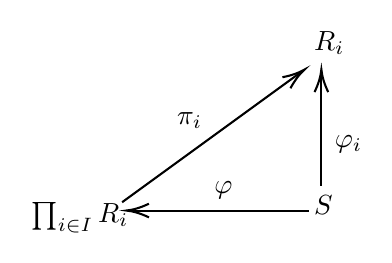
\begin{tikzpicture}[x=0.75pt,y=0.75pt,yscale=-1,xscale=1]
%uncomment if require: \path (0,476); %set diagram left start at 0, and has height of 476

%Straight Lines [id:da7996461945512099] 
\draw    (370,260) -- (284,260) ;
\draw [shift={(282,260)}, rotate = 360] [color={rgb, 255:red, 0; green, 0; blue, 0 }  ][line width=0.75]    (10.93,-3.29) .. controls (6.95,-1.4) and (3.31,-0.3) .. (0,0) .. controls (3.31,0.3) and (6.95,1.4) .. (10.93,3.29)   ;
%Straight Lines [id:da9398415640083908] 
\draw    (376,248) -- (376,194) ;
\draw [shift={(376,192)}, rotate = 90] [color={rgb, 255:red, 0; green, 0; blue, 0 }  ][line width=0.75]    (10.93,-3.29) .. controls (6.95,-1.4) and (3.31,-0.3) .. (0,0) .. controls (3.31,0.3) and (6.95,1.4) .. (10.93,3.29)   ;
%Straight Lines [id:da6839385952780701] 
\draw    (280,256) -- (366.38,193.18) ;
\draw [shift={(368,192)}, rotate = 143.97] [color={rgb, 255:red, 0; green, 0; blue, 0 }  ][line width=0.75]    (10.93,-3.29) .. controls (6.95,-1.4) and (3.31,-0.3) .. (0,0) .. controls (3.31,0.3) and (6.95,1.4) .. (10.93,3.29)   ;

% Text Node
\draw (371,251.4) node [anchor=north west][inner sep=0.75pt]    {$S$};
% Text Node
\draw (235,254.4) node [anchor=north west][inner sep=0.75pt]    {$\prod _{i\in I} R_{i}$};
% Text Node
\draw (323,244.4) node [anchor=north west][inner sep=0.75pt]    {$\varphi $};
% Text Node
\draw (371,172.4) node [anchor=north west][inner sep=0.75pt]    {$R_{i}$};
% Text Node
\draw (381,222.4) node [anchor=north west][inner sep=0.75pt]    {$\varphi _{i}$};
% Text Node
\draw (305,211.4) node [anchor=north west][inner sep=0.75pt]    {$\pi _{i}$};


\end{tikzpicture}
\end{center}
\end{note}
\begin{proof}
We have shown the existence of $\varphi$ in previous chapter. It is easy to verify that $\varphi$ is a homomorphism and therefore $\prod_{i\in I}R_i$ is the product in the category of rings and therefore determined up to isomorphism.
\end{proof}
\begin{theorem}
Let $A_1,A_2,\cdots,A_n$ be ideals in a ring $R$ such that $A_1+A_2+\cdots+A_n=R$ and for each $k$, $A_k\cap(A_1+\cdots+A_{k-1}+A_{k+1}+\cdots+A_n)=0$, then there is a ring isomorphism $R\cong A_1\times A_2\times\cdots\times A_n$.
\end{theorem}
\begin{proof}
By Theorem 2.66 we know that the map $\varphi:A_1\times A_2\times\cdots\times A_n\to R$ given by $(a_1,a_2,\cdots,a_n)\mapsto a_1+a_2+\cdots+a_n$ is an isomorphism of additive abelian groups. It suffices to show that $\varphi$ is a ring homomorphism, which we observe that 
$$
\left( a_1+a_2+\cdots +a_n \right) \left( b_1+b_2+\cdots +b_n \right) =a_1b_1+a_2b_2+\cdots +a_nb_n,
$$
since $a_ib_j\in A_i\cap A_j=0$, therefore $\varphi$ is a ring homomorphism and we finished our proof.
\end{proof}
If $R$ is a ring and $A_1,\cdots,A_n$ are ideals in $R$ that satisfy the hypothesis of Theorem 4.34, then $R$ is said to be the \textbf{(internal) direct product} of the ideals $A_i$. As groups, there are small differences between these two concepts in rings. For example, if a ring $R$ is the internal product of some ideals $A_1,\cdots,A_n$, then each of $A_i$ is actually an ideal contained in $R$ and $R$ is isomorphic to the external product $A_1\times\cdots\times A_n$. However, the external direct product does not contain the $A_i$, it simply contain the copies, say $\iota_i(A_i)$, of each $A_i$. These differences are unimportant in practise, so we often omit the adjective internal or external, and use the following notations: We write $R=\prod A_i$ or $R=A_1\times\cdots\times A_n$ to indicate that the ring $R$ is the internal direct product of its ideals $A_i$.\par
We close this section with a useful result. We first introduce some terminologies. Let $A$ be an ideal in a ring $R$ and $a,b\in R$. The element $a$ is said to be \textbf{congruent} to $b$ modulo $A$ (denoted $a\equiv b(\mathrm{mod}A)$) if $a-b\in A$. Since $R/A$ is a ring, $a_1\equiv a_2(\mathrm{mod}A)$ and $b_1\equiv b_2(\mathrm{mod}A)$ implies $a_1+b_1\equiv a_2+b_2(\mathrm{mod}A)$ and $a_1a_2\equiv b_1b_2(\mathrm{mod}A)$.
\begin{theorem}(Chinese Remainder Theorem)
Let $A_1,\cdots,A_n$ be ideals in a ring $R$ such that $R^2+A_i=R$ for all $i$ and $A_i+A_j=R$ for all $i\ne j$. If $b_1,\cdots,b_n\in R$, then there exists $b\in R$ such that $b\equiv b_i(\mathrm{mod}A_i)$ for all $i=1,2,\cdots,n$. Furthermore $b$ is uniquely determined up to congruence modulo the ideal $A_1\cap\cdots\cap A_n$.
\end{theorem}
\begin{proof}
Since $A_1+A_2=R$ and $A_1+A_3=R$, we have 
$$
R^2=\left( A_1+A_2 \right) \left( A_1+A_3 \right) =A_{1}^{2}+A_1A_3+A_2A_1+A_2A_3\subset A_1+\left( A_2\cap A_3 \right) .
$$
Therefore 
$$
R=A_1+R^2\subset A_1+\left( A_2\cap A_3 \right) \subset R,
$$
whence $R=A_1+(A_2\cap A_3)$. Now we show that $R=A_1+\bigcap_{i\ne 1}A_i$ inductively. Suppose $R=A_1+\left( A_2\cap A_3\cap \cdots \cap A_{k-1} \right) $, then we have 
$$
R^2=\left[ A_1+\left( A_2\cap A_3\cap \cdots \cap A_{k-1} \right) \right] \left( A_1+A_k \right) \subset A_1+\left( A_2\cap A_3\cap \cdots \cap A_k \right) \subset R,
$$
whence $R=A_1+(A_2\cap\cdots\cap A_k)$. Now that $R=A_1+\left( \bigcap_{i\ne 1}{A_i} \right) $ and analogously we may show that $R=A_k+\left( \bigcap_{i\ne k}{A_i} \right) $. Therefore for all $b_k\in R$, there exists $a_k\in A_k$ and $r_k\in\bigcap_{i\ne k}A_i$ such that $b_k=a_k+r_k$, whence $r_k\equiv b_k(\mathrm{mod}A_k)$ for all $k=1,2,\cdots,n$. Observe that $r_i\equiv0(\mathrm{A_j})$ when $i\ne j$, then let $b=r_1+r_2+\cdots+r_n$, we conclude that $b\equiv b_i(\mathrm{mod}A_i)$ for all $i=1,2,\cdots,n$. Now we show that $b$ is uniquely determined up to the congruence modulo $\bigcap A_i$. Suppose $c\equiv b_i(\mathrm{mod}A_i)$, then $b-c\in A_i$ for all $A_i$. Hence $b\equiv c\left( \mathrm{mod}\bigcap_{i=1}^n{A_i} \right) $, we finished our proof.
\end{proof}
The Chinese Remainder Theorem is so named because it is a generalization of the following fact from elementary number theory, which is known to the Chinese mathematicians in the first century A.D.
\begin{corollary}
Let $m_1,m_2,\cdots,m_n$ be positive integers such that $(m_i,m_j)=1$ for $i\ne j$. If $b_1,b_2,\cdots,b_n$ are any integers, then the system of congruences $x=b_i(\mathrm{mod}m_i)$ has an integral solution that is uniquely determined modulo $m=m_1m_2\cdots m_n$.
\end{corollary}
\begin{proof}
Let $A_i=(m_i)$. Clearly $\bigcap A_i=(m)$ and $(m_i,m_j)=1$ implies $A_i+A_j=\mathbb{Z}$. Then the result follows from the Chinese Remainder Theorem.
\end{proof}
\begin{corollary}
If $A_1,A_2,\cdots,A_n$ are ideals of $R$, then there exists a monomorphism of rings 
$$
\theta :R/\left( A_1\cap A_2\cap \cdots \cap A_n \right) \rightarrow R/A_1\times R/A_2\times \cdots \times R/A_n.
$$
If $R^2+A_i=R$ for all $i$ and $A_i+A_j=R$ for all $i\ne j$, then $\theta$ is an isomorphism of rings.
\end{corollary}
\begin{proof}
We first show that there is a monomorphism $\theta$. Define 
$$
\theta _1:R\rightarrow R/A_1\times R/A_2\times \cdots \times R/A_n
$$
given by $r\mapsto(r+A_1,\cdots,r+A_n)$. Clearly the kernel of $\theta_1$ is $\bigcap A_i$. Therefore by the First Isomorphism Theorem we have the monomorphism 
$$
\theta :R/\left( A_1\cap A_2\cap \cdots \cap A_n \right) \rightarrow R/A_1\times R/A_2\times \cdots \times R/A_n.
$$
Now we show that under the given condition $\theta$ is an isomorphism. In fact, let 
$$
\left( b_1+A_1,\cdots ,b_n+A_n \right) \in R/A_1\times R/A_2\times \cdots \times R/A_n,
$$
there exists $b\in R$ such that $b\equiv b_i(\mathrm{mod}A_i)$ for all $i=1,2,\cdots,n$. Hence 
$$
\theta \left( b+\bigcap{A_i} \right) =\left( b+A_1,\cdots ,b+A_n \right) =\left( b_1+A_1,\cdots ,b_n+A_n \right) ,
$$
and therefore $\theta$ is an epimorphism.
\end{proof}
\begin{center}
\begin{large}
    \textbf{Exercises for 4.2}
\end{large}
\end{center}
\begin{problem}\em
The set of all nilpotent elements in a commutative ring forms an ideal.
\end{problem}
\begin{proof}
Let $I=\{r\in R:r^n=0\ \text{for some}\ n\in\mathbb{N}\}$. Then let $r\in R$ and $i\in I$, we have $(ir)^n=i^nr^n=0$, hence $ir\in I$. Therefore $I$ is a right ideal of $R$. Similarly we may show that $I$ is a left ideal of $R$, and hence an ideal.
\end{proof}
\begin{problem}\em
Let $I$ be an ideal in a commutative ring $R$ and let $\mathrm{Rad}I=\{r\in R:r^n\in I\ \text{for some}\ n\in\mathbb{N}\}$. Show that $\mathrm{Rad}I$ is an ideal.
\end{problem}
\begin{proof}
Let $j\in\mathrm{Rad}I$ and $j^n=i\in I$. Suppose $r\in R$, then $(jr)^n=j^nr^n=ir^n\in I$, hence $jr\in\mathrm{Rad}I$, therefore $\mathrm{Rad}I$ is a right ideal of $R$. Similarly we may show that $\mathrm{Rad}I$ is a left ideal of $R$, and hence an ideal.
\end{proof}
\begin{problem}\em
If $R$ is a ring and $a\in R$, then $J=\{r\in R:ra=0\}$ is a left ideal and $K=\{r\in R:ar=0\}$ is a right ideal in $R$.
\end{problem}
\begin{proof}
We first show that $J$ is a left ideal of $R$. Let $j\in J$, then for all $r\in R$, we have $rj\in J$ since $rja=r(ja)=0$, and hence $J$ is a left ideal of $R$. Similarly we may prove that $K$ is a left ideal of $R$.
\end{proof}
\begin{problem}\em
If $I$ is a left ideal in a ring $R$, then $A(I)=\{r\in R:rx=0\ \text{for every}\ x\in I\}$ is an ideal in $R$.
\end{problem}
\begin{proof}
Let $a\in A(I)$. Then for all $r\in R$, we show that $ar\in A(I),ra\in A(I)$. First, $arx=ar^\prime=0$ since $I$ is a left ideal of $R$ implies $rx=r^\prime\in I$, then by the definition of $A(I)$ we conclude that $ar\in A(I)$. Then $rax=r0=0$ since $a\in A(I)$ and $x\in I$, therefore $A(I)$ is an ideal of $R$.
\end{proof}
\begin{problem}\em
If $I$ is an ideal in a ring $R$, let $[R:I]=\{r\in R:xr\in I\ \text{for all}\ x\in R\}$. Show that $[R:I]$ is an ideal which contains $I$.
\end{problem}
\begin{proof}
Let $a\in[R:I]$ and $r\in R$. Then $xar=\left( xa \right) r=ir\in I$, where $i\in I$ and by the fact that $I$ is an ideal we conclude that $ar\in[R:I]$. Also observe that $xra=(xr)a\in I$, we have $ra\in I$ and hence $[R:I]$ is an ideal of $R$. Clearly for all $i\in I$, we have $xi\in I$ for all $x\in R$, hence $I\subset[R:I]$.
\end{proof}
\begin{problem}\em
(a) The center of the ring $S$ of all $2\times 2$ matrices over a field $F$ consists of all matrices of the form $
\left( \begin{matrix}
	a&		0\\
	0&		a\\
\end{matrix} \right) 
$.\par
(b) The center of $S$ is not an ideal of $S$.\par
(c) What is the center of the ring of all $n\times n$ matrices over a division ring?
\end{problem}
\begin{proof}
(a) Observe that 
$$
\left\{ \begin{array}{c}
	\left( \begin{matrix}
	a&		b\\
	c&		d\\
\end{matrix} \right) \left( \begin{matrix}
	1&		0\\
	0&		0\\
\end{matrix} \right) =\left( \begin{matrix}
	a&		0\\
	c&		0\\
\end{matrix} \right) ,\\
	\left( \begin{matrix}
	1&		0\\
	0&		0\\
\end{matrix} \right) \left( \begin{matrix}
	a&		b\\
	c&		d\\
\end{matrix} \right) =\left( \begin{matrix}
	a&		b\\
	0&		0\\
\end{matrix} \right) ,\\
\end{array} \right. \Rightarrow b=c=0;\left\{ \begin{array}{c}
	\left( \begin{matrix}
	a&		b\\
	c&		d\\
\end{matrix} \right) \left( \begin{matrix}
	0&		1\\
	0&		0\\
\end{matrix} \right) =\left( \begin{matrix}
	0&		a\\
	0&		0\\
\end{matrix} \right) ,\\
	\left( \begin{matrix}
	0&		1\\
	0&		0\\
\end{matrix} \right) \left( \begin{matrix}
	a&		b\\
	c&		d\\
\end{matrix} \right) =\left( \begin{matrix}
	0&		d\\
	0&		0\\
\end{matrix} \right) ,\\
\end{array} \right. \Rightarrow a=d.
$$
Therefore elements in the center of $S$ must have the form $
\left( \begin{matrix}
	a&		0\\
	0&		a\\
\end{matrix} \right) 
$. Now we show that all matrices of the form $
\left( \begin{matrix}
	a&		0\\
	0&		a\\
\end{matrix} \right) 
$ is in the center of $S$. Observe that 
$$
\left( \begin{matrix}
	a&		0\\
	0&		a\\
\end{matrix} \right) \left( \begin{matrix}
	x&		y\\
	z&		w\\
\end{matrix} \right) =\left( \begin{matrix}
	x&		y\\
	z&		w\\
\end{matrix} \right) \left( \begin{matrix}
	a&		0\\
	0&		a\\
\end{matrix} \right) =\left( \begin{matrix}
	ax&		ay\\
	az&		aw\\
\end{matrix} \right) .
$$\par
(b) Let $C$ denote the center of $S$. Observe that 
$$
\left( \begin{matrix}
	a&		0\\
	0&		a\\
\end{matrix} \right) \left( \begin{matrix}
	1&		0\\
	0&		0\\
\end{matrix} \right) =\left( \begin{matrix}
	a&		0\\
	0&		0\\
\end{matrix} \right) \notin C,
$$
hence $C$ is not an ideal of $S$.\par
(c) Similar to (b) we may show that the center of all $n\times n$ matrices over a field consists of all elements $aE_n$, where $E_n=\mathrm{diag}\{1,\cdots,1\}$. Observe that $aE_n$ has an inverse $\frac{1}{a}E_n$, hence it is an element of all $n\times n$ matrices over a division ring. Therefore the center of which is $\{aE_n:a\in D\}$.
\end{proof}
\begin{problem}\em
(a) A ring $R$ with identity is a division ring if and only if $R$ has no proper left ideals.\par
(b) If $S$ is a ring with no proper left ideals, then either $S^2=0$ or $S$ is a division ring.
\end{problem}
\begin{proof}
(a) Let $R$ be a division ring. Then for all $S$ subring of $R$ that do not contain $1_R$, every $s\in S$ has an inverse $s^{-1}\in R$ such that $s^{-1}s=1_R\notin S$, hence $S$ is not an ideal of $R$. Therefore an ideal of $R$ must contain $1_R$, which is the trivial ideal of $R$. Conversely, suppose $R$ has only trivial ideal $R$, then for all $r\in R$, there exists some $s\in R$ such that $rs=1_R$, hence $R$ is a division ring.\par
(b) Suppose that $S^2\ne S$, we show that $S$ is a division ring, which suffices to show that $S$ has an identity. Consider $I=\{a\in S:Sa=0\}$, which is easily to be proved an ideal of $S$. Therefore $I=0$ or $I=S$. By the given condition we know that $I=0$, hence $Sa=0$ if and only if $a=0$. Therefore for each nonzero element $a\in S$, we have $Sa=S$, and this implies right cancellation, since $(x-y)s=0$ implies $x-y=0$, which is $x=y$ when $s$ is a nonzero element. Now $Sa=S$, hence there exists some $e\in S$ such that $ea=a$, and $e^2a=ea$. $a$ is a nonzero element, hence by the right cancellation we have $e^2=e$. Clearly $e\ne 0$, therefore $e$ is an identity element of $S$, whence $S$ is a division ring.
\end{proof}
\begin{problem}\em
Let $R$ be a ring with identity and $S$ the ring of all $n\times n$ matrices over $R$. $J$ is an ideal of $S$ if and only if $J$ is a ring of all $n\times n$ matrices over $I$ for some ideal $I$ in $R$.
\end{problem}
\begin{proof}
Let $J$ be an ideal of $S$, let $I$ be the set of all elements that appears in the matrices of $J$. To show that $I$ is an ideal of $R$, it suffices to show that for all $a\in I$ and $E_{ij}$, which denote the matrix with element $1_R$ at position $(i,j)$ and $0$ in other, $aE_{ij}\in J$. Now choose $B\in J$ such that $b_{st}=a$. Observe that 
$$
E_{is}BE_{tj}=\sum_{u,v}{b_{uv}E_{is}E_{uv}E_{tj}}=\sum_{u,v}{b_{uv}\delta _{su}\delta _{vt}E_{ij}}=aE_{ij}\in J,
$$
where $B=\sum_{u,v}b_{uv}E_{uv}\in J$ and $\delta_{ij}$ is the Kronecker symbol, we conclude that $I$ is an ideal of $R$.
\end{proof}
\begin{problem}\em
Let $S$ be the ring of all $n\times n$ matrices over a division ring $D$.\par
(a) $S$ has no proper ideals.\par
(b) $S$ has zero divisors. Consequently, $S\cong S/0$ is not a division ring and $0$ is a prime ideal.
\end{problem}
\begin{proof}
(a) Suppose $J$ is an ideal of $S$. Then by Exercise 4.25 we know that the elements of matrices in $J$ is an ideal of $D$, which is a division ring and has to be trivial. Therefore $J$ is the trivial ideal of $S$. which is not proper.\par
(b) Consider 
$$
\left( \begin{matrix}
	1&		&		&		\\
	&		1&		&		\\
	&		&		\ddots&		\\
	&		&		&		1\\
\end{matrix} \right) \left( \begin{matrix}
	&		&		&		1\\
	&		&		&		\\
	&		&		&		\\
	&		&		&		\\
\end{matrix} \right) =0\in S.
$$
Therefore $S$ has zero divisors and $S\cong S/0$ is not a division ring with $0$ is a prime ideal.
\end{proof}
\begin{note}\em
The example in this exercise does not satisfy condition given in Theorem 4.25.
\end{note}
\begin{problem}\em
(a) Show that $\mathbb{Z}$ is a principal ideal ring.\par
(b) Every homomorphic image of a principal ideal ring is also a principal ideal ring.\par
(c) $\mathbb{Z}_m$ is a principal ideal ring for every $m>0$.
\end{problem}
\begin{proof}
(a) Let $I$ be an ideal of $\mathbb{Z}$, then $I$ is a subring of $\mathbb{Z}$. By Theorem 2.15 we conclude that $I$ is of the form $m\mathbb{Z}$, where $m\in\mathbb{Z}$. Therefore $I=(m)$, which is a principal ideal. Since this is true for all ideals of $\mathbb{Z}$, we showed that $\mathbb{Z}$ is a principal ideal domain.\par
(b) Let $R$ be a principal ideal ring and $f:R\to S$ is a homomorphism. Suppose $S=\mathrm{Im}f$, we now show that $S$ is a principal ideal ring. Let $I=(m)$ is an ideal of $R$, that is, for all $r\in R$ we have $rI\subset I$. Therefore $f(rI)=f(r)f(I)\subset f(I)$ and hence $f(I)$ is an ideal of $S$. Since $I=(m)$, we have $f(I)=(f(m))$ by Theorem 4.15, therefore $f(I)$ is a principal ideal of $S$. Since this is true for all ideals of $S$, we conclude that $S$ is a principal ideal ring.\par
(c) This is a direct corollary of (b).
\end{proof}
\begin{problem}\em
If $N$ is the ideal of all nilpotent elements in a commutative ring $R$, then $R/N$ is a ring with no nonzero nilpotent elements.
\end{problem}
\begin{proof}
Suppose $r+N\in R/N$ and $(r+N)^n=r^n+N=r+N$. Then $r^n=r$, hence $r\in N$. Therefore $R/N$ has no nonzero nilpotent elements.
\end{proof}
\begin{problem}\em
Let $R$ be a ring without identity and with no zero divisors. Let $S$ be the ring whose additive group is $R\times\mathbb{Z}$ as in the proof of Theorem 4.10. Let $A:\{(r,n)\in S:rx+nx=0\ \text{for every}\ x\in R\}$.\par
(a) $A$ is an ideal in $S$.\par
(b) $S/A$ has an identity and contains a subring isomorphic to $R$.\par
(c) $S/A$ has no zero divisors.
\end{problem}
\begin{proof}
(a) This is easy to verify through definition.\par
(b) Let $a\in A$, then clearly $aA$ is an identity of $S/A$. Now we define $f:S\to R$ given by $(a,b)\mapsto a$, which is an epimorphism. Therefore by the First Isomorphism Theorem $f$ induces an epimorphism $\overline{f}:S/A\to R$, which implies that $S/A$ has an subring isomorphic to $R$.\par
(c) If not, then there exists some $(r,n)(s,m)\in A$ and $(r,n),(s,m)\notin A$. Therefore $(rs+mr+ns,nm)\in A$, whence for all $x\in S$, we have 
$$(rs+mr+ns)x+(nm)x=rsx+mrx+nsx+nmx=0.$$
Since $(s,m)\notin A$, we have $sx+mx\ne 0$ for some $x\in R$. Denote $sx+mx=t$. Now it suffices to show that $rx+nx=0$ for all $x\in R$. Now observe that 
$$rt+nt=0\Leftrightarrow t(rt+nt)=0\Leftrightarrow trt+nt^2=0\Leftrightarrow (tr+nt)t=0\Leftrightarrow tr+nt=0,$$
then we may conclude that 
$$tr+nt=0\Leftrightarrow trx+ntx=0\Leftrightarrow t(rx+nx)=0\Leftrightarrow rx+nx=0,$$
which finished the proof.
\end{proof}
\begin{problem}\em
Let $f:R\to S$ be a homomorphism of rings, $I$ an ideal in $R$, and $J$ an ideal in $S$.\par
(a) $f^{-1}(J)$ is an ideal in $R$ that contains $\mathrm{Ker}f$.\par
(b) If $f$ is an epimorphism, then $f(I)$ is an ideal in $S$. If $f$ is not surjective, $f(I)$ need not be an ideal in $S$.
\end{problem}
\begin{proof}
(a) Since the kernel is the smallest ideal of $R$, it suffices to show that $f^{-1}(J)$ is an ideal. Let $r\in R$. Then there exists some $s\in S$ such that $f^{-1}(s)=r$. Therefore $rf^{-1}(J)=f^{-1}(x)f^{-1}(J)=f^{-1}(xJ)\subset f^{-1}(J)$, whence $f^{-1}(J)$ is a right ideal of $R$. This is true for left ideal, hence $f^{-1}(J)$ is an ideal of $R$.\par
(b) Let $s\in S$. Since $f$ is an epimorphism, we have $f(r)=s$ for some $r\in R$. Therefore $sf(I)=f(r)f(I)=f(rI)\subset f(I)$, hence $f(I)$ is a right ideal of $S$. This is also true for left ideal, hence $f(I)$ is an ideal of $S$. Now consider the injective homomorphism $f:\mathbb{Z}\to\mathbb{Q}$, clearly $2\mathbb{Z}$ is an ideal of $\mathbb{Z}$, but $f(2\mathbb{Z})=2\mathbb{Z}$ is not an ideal of $\mathbb{Q}$.
\end{proof}
\begin{problem}\em
If $P$ is an ideal in a not necessarily commutative ring $R$, then the following conditions are equivalent.\par
(a) $P$ is a prime ideal.\par
(b) If $r,s\in R$ are such that $rRs\subset P$, then $r\in P$ or $s\in P$.\par
(c) If $(r)$ and $(s)$ are principal ideals of $R$ such that $(r)(s)\subset P$, then $r\in P$ or $s\in P$.\par
(d) If $U$ and $V$ are right ideals such that $UV\subset P$, then $U\subset P$ or $V\subset P$.\par
(e) If $U$ and $V$ are left ideals such that $UV\subset P$, then $U\subset P$ or $V\subset P$.
\end{problem}
\begin{proof}
We first show that (a), (b) and (c) are equivalent.\par
(a)$\Rightarrow$(b): Suppose $P$ is a prime ideal, then if $(RrR)(RsR)\subset P$, we have $(RrR)\subset P$ or $(RsR)\subset P$. Say $(RrR)\subset P$. Observe that $RrR$ is an ideal of $R$, hence $(RrR)=RrR$. Now consider $(r)=A$, since $A^3\subset RrR\subset P$ we have $(r)^3\subset P$, whence $r\in A\subset P$. Hence $r\in P$.\par
(a)$\Rightarrow$(c): This is trivial.\par
(c)$\Rightarrow$(b): Since $(r)$ is an ideal of $R$, then $(r)R(s)\subset P$, whence $rRs\subset P$. Then by (b) we conclude that $r\in P$ or $s\in P$.\par
(b)$\Rightarrow$(a): Suppose $A,B$ are ideals of $P$ such that $AB\subset P$, but neither $A\subset P$ nor $B\subset P$. Then let $a\in P\setminus A$ and $b\in P\setminus B$, we have $aRb\subset P$, a contradiction!\par
Now we show that (a), (d) and (e) are equivalent. Since the proof of right ideals are analogous to that of left ideals, we only show (a) and (d) are equivalent.\par
(a)$\Rightarrow$(d): Let $A,B$ be left ideals of $R$ such that $AB\subset P$ and $A\not\subset P$. Then there exists some $a\in A\setminus P$ such that $aB\subset P$, whence $ab\in P$ for all $b\in B$. This shows $b\in P$ by the property of a prime ideal, and hence $B\subset P$ since this is true for all $b\in B$.\par
(d)$\Rightarrow$(a): Trivial.
\end{proof}
\begin{problem}\em
The set consisting of zero and all zero divisors in a commutative ring with identity contains at least one prime ideal.
\end{problem}
\begin{proof}
We introduce a Theorem that will be proved in commutative algebra:\par
\textbf{Theorem}: If $S$ is a multiplicative subset of a ring $R$ which is disjoint from an ideal $I$ of $R$, then there exists an ideal $P$ which is maximal in the set of all ideals of $R$ disjoint from $S$ and containing $I$. Furthermore, $P$ is prime.\par
Now let $Z=\{a\in R:a\ne0,ab\ne 0\ \text{for all}\ 0\ne b\in R\}$. Consider $S=R-Z$. By the theorem above it suffices to show that $S$ is multiplicative. Let $ab\in S$. By the definition of $S$ we have $a,b$ are both not zero divisors. Now suppose $ab$ is a zero divisor, then there exists some $c\in R$ such that $c(ab)=0$. Since $R$ is commutative, we have $a(cb)=0$, which contradict to the fact that $b$ is not a zero divisor, hence $S$ is multiplicative and we finished our proof.
\end{proof}
\begin{problem}\em
Let $R$ be a commutative ring with identity and suppose that the ideal $A$ of $R$ is contained in a finite union of prime ideals $P_1\cup P_2\cup\cdots\cup P_n$. Show that $A\subset P_i$ for some $i$.
\end{problem}
\begin{proof}
We prove by contradiction. Suppose $A\not\subset P_i$ for all $i\in\{1,2,\cdots,n\}$, then $A\cap P_i\cap\left(\bigcap_{j\ne i}P_j\right)\ne\emptyset$ for all $i\in\{1,2,\cdots,n\}$. Now choose $a_i\in(A\cap P_i)\setminus\left(\bigcup_{j\ne i}P_j\right)$, we have $a_1+a_2a_3\cdots a_n\in A$, but not in $\bigcup_{i=1}^nP_i$, a contradiction!
\end{proof}
\begin{problem}\em
Let $f:R\to S$ be an epimorphism of rings with kernel $K$.\par
(a) If $P$ is a prime ideal in $R$ that contains $K$, then $f(P)$ is a prime ideal in $S$.\par
(b) If $Q$ is a prime ideal in $S$, then $f^{-1}(Q)$ is a prime ideal in $R$ that contains $K$.\par
(c) There is a one-to-one correspondence between the set of all prime ideals in $R$ that contains $K$ and the set of all prime ideals in $S$, given by $P\mapsto f(P)$.\par
(d) If $I$ is an ideal in a ring $R$, then every prime ideal in $R/I$ is of the form $P/I$, where $P$ is a prime ideal in $R$ that contains $I$.
\end{problem}
\begin{proof}
(a) Clearly $f(P)$ is an ideal of $S$, it suffices to show that $f(P)$ is a prime ideal of $S$. The epimorphism $f:R\to S$ induces an isomorphism $\overline{f}:R/K\to S$, hence it suffices to show that $P/K$ is a prime ideal of $R/K$. Let $(A/K)(B/K)\subset P/K$, then $AB/K\subset P/K$, whence $AB+K\subset P+K$, which is $AB\subset P$. Since $P$ is a prime ideal of $R$, we have $A\subset P$ or $B\subset P$, hence $P/K$ is a prime ideal of $S$ and we finished our proof.\par
(b) The proof of which is similar to (a).\par
(c) Since $f:R\to S$ induces an isomorphism $\overline{f}:R/K\to S$, and if $P$ is an ideal of $R$, we have $P/K$ is an ideal of $S$, hence we have the one-to-one correspondence $P\mapsto f(P)$ of prime ideals of $R$ and prime ideals of $S$.\par
(d) Observe that the ideal of $R/I$ is of the form $J/I$, where $J$ is an ideal of $R$, therefore $P/I$ is an ideal of $R/I$ when $P$ is a prime ideal of $R$. Then consider the canonical injection $\pi:R\to R/I$, we have $\pi^{-1}(P/I)=P$, then by (b) we conclude that the prime ideal of $R/I$ is of the form $P/I$.
\end{proof}
\begin{problem}\em
An ideal $M\ne R$ in a commutative ring $R$ with identity is maximal if and only if for every $r\in R-M$, there exists $x\in R$ such that $1_R-rx\in M$.
\end{problem}
\begin{proof}
Suppose $M$ is maximal. Then for $r\in R-M$, consider the ideal $(M,r)$. Since $M$ is maximal and $(M,r)\supset M$, we conclude that $(M,r)=R$ for $M$ is the maximal ideal of $R$. Since $R$ is a commutative ring, we have $m+rx\in R$. In particular, $1_R\in R$ and hence $m+rx=1_R$ for some $x\in R$. Conversely, we show that $R/M$ is a division ring. Clearly $1_RM$ is the identity of $R/M$. Now it suffices to show that each $r+M\in R/M$ is a unit. This follows by the fact that $rx\equiv 1_R(\mathrm{mod}M)$ for some $x$ and hence we finished our proof.
\end{proof}
\begin{problem}\em
The ring $E$ of even integers contains a maximal ideal $M$ such that $E/M$ is not a field.
\end{problem}
\begin{proof}
Consider $M=(4)$, which we now show is a maximal ideal of $E$. Clearly $M$ is an ideal of $E$. Suppose $I$ is another ideal of $E$ and $M\subset I\subset E$, we have $4k+2\in I$ or otherwise $I\subset M$. Therefore $(M,2)\subset I$ and $(M,2)=E$, which implies that $M$ is the maximal ideal of $E$. However $E/M$ has no identity. The only two elements of $E/M$ are $\overline{2}$ or $\overline{4}$. However $\overline{2}\times\overline{2}=\overline{4}\times\overline{2}=\overline{4}$, which shows that $E/M$ has no identity element.
\end{proof}
\begin{problem}\em
In the ring $\mathbb{Z}$ the following conditions on a nonzero ideal $I$ are equivalent:\par
(i) $I$ prime; (ii) $I$ is maximal; (iii) $I=(p)$ with $p$ prime.
\end{problem}
\begin{proof}
(i)$\Rightarrow$(ii): Suppose $I$ is a prime ideal. Since $\mathbb{Z}$ is principal ideal domain, we suppose $I=(p)$. Suppose $ab\subset (p)$, then $p\mid ab$. Since $I$ is a prime ideal, we have $p\mid a$ or $p\mid b$. Therefore $p$ is prime. Now suppose $J$ is another ideal contains $I$, then $J=(1)$ since $I$ is prime, hence $J=\mathbb{Z}$ and $I$ is maximal.\par
(ii)$\Rightarrow$(iii): Suppose $I=(p)$ and $p$ is not prime, then there exists some prime $p_1$ such that $p=kp_1$. Consider $(p_1)$, which is an ideal that contains $I$ but not equal to $\mathbb{Z}$, which contradict to the fact that $I$ is maximal. Hence $p$ is prime.\par
(iii)$\Rightarrow$(i): Suppose $ab\in (p)$. Since $p$ is prime, we have $p\mid a$ or $p\mid b$, therefore $a\in (p)$ or $b\in (p)$. Therefore $(p)$ is prime.
\end{proof}
\begin{problem}\em
Determine all prime and maximal ideals in the ring $\mathbb{Z}_m$.
\end{problem}
\begin{proof}
Since $\mathbb{Z}_m=\mathbb{Z}/m\mathbb{Z}$, by Exercise 4.34(d) we know that the prime ideals of $\mathbb{Z}_m$ are of the form $p\mathbb{Z}/m\mathbb{Z}$, where $p\mid m$. The maximal ideals of $\mathbb{Z}_m$ are precisely the prime ideals.
\end{proof}
\begin{problem}\em
If $R_1,\cdots,R_n$ are rings with identity and $I$ is an ideal in $R_1\times R_2\times\cdots\times R_n$, then $I=A_1\times A_2\times\cdots\times A_m$, where $A_i$ is an ideal in $R_i$.\par
\end{problem}
\begin{proof}
Consider the canonical epimorphism $\pi_k:R_1\times R_2\times\cdots\times R_n\to R_k$, then let $A_k=\pi_k(I)$, we have $A_k$ an ideal of $R_k$ and $I=A_1\times A_2\times\cdots\times A_n$.\par
\end{proof}
\begin{note}\em
Note that the conclusion may be false if the rings $R_i$ does not have identities.
\end{note}
\begin{problem}\em
An element $e$ in a ring $R$ is said to be \textbf{idempotent} if $e^2=e$. An element of the center of the ring $R$ is said to be \textbf{central}. If $e$ is a central idempotent in a ring $R$ with identity, then\par
(a) $1_R-e$ is a central idempotent;\par
(b) $eR$ and $(1_R-e)R$ are ideals in $R$ such that $R=eR\times(1_R-e)R$.
\end{problem}
\begin{proof}
(a) First we observe that 
$$
\left( 1_R-e \right) ^2=\left( 1_R-e \right) \left( 1_R-e \right) =1_R-e-e+e^2=1_R-e,
$$
hence $1_R-e$ is a idempotent element. Also observe that 
$$
\left( 1_R-e \right) r=r-er=r-re=r\left( 1_R-e \right) ,
$$
we conclude that $1_R-e$ is a central idempotent.\par
(b) We first show that $eR$ is an ideal of $R$. Let $er\in eR$, then $r^\prime er=er^\prime r\in eR$, hence $eR$ is an ideal of $R$. Also we may verify that $(1_R-e)R$ is an ideal of $R$. Now that $er+(1_R-e)r=er+r-er=r\in R$, hence $R=eR\times(1_R-e)R$.
\end{proof}
\begin{problem}\em
Idempotent elements $e_1,\cdots,e_n\in R$ are said to be \textbf{orthogonal} if $e_ie_j=0$ for $i\ne j$. If $R_1,\cdots,R_n$ are rings with identity, then the following conditions are equivalent:\par
(a) $R\cong R_1\times R_2\times\cdots\times R_n$;\par
(b) $R$ contains a set of orthogonal central idempotents $\{e_1,\cdots,e_n\}$ such that $e_1+\cdots+e_n=1_R$ and $e_iR\cong R_i$ for each $i$.\par
(c) $R$ is the internal direct product $R=A_1\times A_2\times\cdots\times A_n$, where $A_i$ is an ideal of $R$ such that $A_i\cong R_i$.
\end{problem}
\begin{proof}
(a)$\Rightarrow$(b): Let $\overline{e_i}=(0,\cdots,1_R,\cdots,0)$, then $\overline{e_i}\in R_1\times R_2\times\cdots\times R_n$, and $\sum\overline{e_i}=1_R$. Clearly $\{\overline{e_1},\cdots,\overline{e_n}\}$ are orthogonal and $\overline{e_i}R\cong R_i$.\par
(b)$\Rightarrow$(c): Let $A_k=e_kR$, observe that $A_k$ is then the principal ideal $(e_k)$ of $R$ and $A_k$ itself is a ring with identity $e_k$.\par
(c)$\Rightarrow$(a): Trivial.
\end{proof}
\begin{problem}\em
If $m\in\mathbb{Z}$ has a prime decomposition $m=p_1^{k_1}\cdots p_t^{k_t}$ where $k_i>0$ and $p_i$ are primes, then there is an isomorphism of rings $\mathbb{Z}_m\cong\mathbb{Z}_{p_1^{k_1}}\times\cdots\times\mathbb{Z}_{p_t^{k_t}}$.
\end{problem}
\begin{proof}
We first show that $\mathbb{Z}^2+p_i^{k_i}\mathbb{Z}=\mathbb{Z}$ for all $i$. This is trivial since for all $m\in\mathbb{Z}$, we have $(m-p_i^{k_i})+p_i^{k_i}=m$. Now we show that $p_i^{k_i}\mathbb{Z}+p_j^{k_j}\mathbb{Z}=\mathbb{Z}$. Since $(p_i^{k_i},p_j^{k_j})=1$, by Bezout's Theorem we have $mp_i^{k_i}+np_j^{k_j}=1$. Hence for all $r\in\mathbb{Z}$ we have $rmp_i^{k_i}+rnp_j^{k_j}=r$. Now by Corollary 4.37 we have
$$
\theta :\mathbb{Z} /\left( p_{1}^{k_1}\mathbb{Z} \cap \cdots \cap p_{t}^{k_t}\mathbb{Z} \right) \rightarrow \mathbb{Z} /p_{1}^{k_1}\mathbb{Z} \times \cdots \times \mathbb{Z} /p_{t}^{k_t}\mathbb{Z} 
$$
is an isomorphism. Hence
$$
\mathbb{Z} _m=\mathbb{Z} /m\mathbb{Z} \cong \mathbb{Z} /\left( p_{1}^{k_1}\mathbb{Z} \cap \cdots \cap p_{t}^{k_t}\mathbb{Z} \right) \cong \mathbb{Z} /p_{1}^{k_1}\mathbb{Z} \times \cdots \times \mathbb{Z} /p_{t}^{k_t}\mathbb{Z} =\mathbb{Z} _{p_{1}^{k_1}}\times \cdots \times \mathbb{Z} _{p_{t}^{k_t}}.
$$
\end{proof}
\subsection{Factorization in Commutative Rings}
In this section, we shall extend the concept of divisibility, greatest common divisor and prime in the ring of integers to arbitrary commutative rings and study those integral domains in which an analogue of the Fundamental Theorem of Arithmetic holds. The chief result is that every PID is UFD. In addition we study those commutative rings in which an analogue of the division algorithm is valid(Euclidean rings).
\begin{definition}
A nonzero element $a$ of a commutative ring $R$ is said to be \textbf{divide} an element $b\in R$, if there exists $x\in R$ such that $ax=b$. Elements $a,b\in R$ are said to be \textbf{associates} if $a\mid b$ and $b\mid a$.
\end{definition}
Virtually all statements about divisibility may be phrased in terms of principal ideals as we shall see.
\begin{theorem}
Let $a,b$ and $u$ be elements of a commutative ring $R$ with identity.\par
(i) $a\mid b$ if and only if $(b)\subset (a)$.\par
(ii) $a$ and $b$ are associates if and only if $(a)=(b)$.\par
(iii) $u$ is a unit if and only if $u\mid r$ for all $r\in R$.\par
(iv) $u$ is a unit if and only if $(u)=R$.\par
(v) The relation "$a$ is associates with $b$" is an equivalence relation on $R$.\par
(vi) If $a=br$ with $r\in R$ a unit, then $a$ and $b$ are associates. If $R$ is an integral domain, the converse id true.
\end{theorem}
\begin{proof}
(i) Suppose $a\mid b$, then $b=ax$ for some $x\in R$. Therefore we have $\left( b \right) =bR=axR\subset aR=\left( a \right) $ and hence $(b)\subset(a)$. Conversely, if $(b)\subset (a)$, then $bR\subset aR$ and hence there exists some $x\in R$ such that $b=ax$. Therefore $a\mid b$.\par
(ii) If $a$ and $b$ associates, we have $a\mid b$ and $b\mid a$. Hence $(a)\subset (b)\subset (a)$ and therefore $(a)=(b)$. Conversely, if $(a)=(b)$, then $(a)\subset (b)$ and $(b)\subset (a)$. Therefore $a\mid b$ and $b\mid a$, whence $a$ and $b$ are associates.\par
(iii) Suppose $u$ is a unit, then there exists some $v\in R$ such that $uv=1_R$. Now for all $r\in R$, we have $rv\in R$ such that $urv=r$, therefore $u\mid r$. Conversely, suppose $u\mid r$ for all $r\in R$, let $r=1_R$, we have $uv=1_R$ for some $v\in R$, therefore $u$ is a unit.\par
(iv) Let $u$ be a unit, then $u\mid 1_R$. Hence $(1_R)\subset (u)$. However $(1_R)=R$, hence $(u)=R$. Conversely, if $(u)=R$, then for all $r\in R$, there exists $v\in R$ such that $uv=r$, therefore $u$ is a unit.\par
(v) Verify by definition.\par
(vi) Since $a=br$, we have $b\mid a$. However $u$ is a unit, therefore there exists some $v\in R$ such that $av=b$, whence $a\mid b$. Hence $a$ and $b$ associates. Conversely, suppose $R$ is an integral domain, then we have $u,v\in R$ such that $a=bu$ and $b=av$. Therefore $a=avu$. Since $R$ is an integral domain, we have $vu=1_R$, hence $u$ is a unit.
\end{proof}
\begin{definition}
Let $R$ be a commutative ring with identity. An element $c$ of $R$ is \textbf{irreducible} provided that:\par
(i) $c$ is a nonzero nonunit;\par
(ii) $c=ab$ implies $a$ or $b$ is a unit.\par
An element $p$ of $R$ is \textbf{prime} provided that:\par
(i) $p$ is a nonzero nonunit;\par
(ii) $p\mid ab$ implies $p\mid a$ and $p\mid b$.
\end{definition}
Here are some examples.
\begin{example}\em
If $p$ is a prime number in $\mathbb{Z}$, then both $p$ and $-p$ are irreducible and prime in $\mathbb{Z}$. In the ring $\mathbb{Z}_6$, $\overline{2}$ is prime but not irreducible, since $\overline{2}=\overline{2}\cdot\overline{4}$, however both $\overline{2}$ and $\overline{4}$ are zero divisors. We will give an example of an irreducible element which is not prime in exercises.
\end{example}
There is a close connection between prime [resp. irreducible] elements in a ring $R$ and prime [resp. maximal] ideals in $R$.
\begin{theorem}
Let $p$ and $c$ be nonzero elements in an integral domain $R$.\par
(i) $p$ is prime if and only if $(p)$ is nonzero prime ideal.\par
(ii) $c$ is irreducible if and only if $(c)$ is maximal in the set $S$ of all proper principal ideals of $R$.\par
(iii) Every prime element of $R$ is irreducible.\par
(iv) If $R$ is a PID, then $p$ is prime if and only if $p$ is irreducible.\par
(v) Every associate of an irreducible [resp. prime] element of $R$ is irreducible [resp. prime].\par
(vi) The only divisors of an irreducible element of $R$ are its associates and the units in $R$.
\end{theorem}
\begin{note}\em
Several parts of Theorem 4.41 are true for any commutative ring with identity as we will see in the following proof.
\end{note}
\begin{proof}
(i) Suppose $p$ is prime. Then $p\mid ab$ implies $p\mid a$ or $p\mid b$. Therefore if $ab\in (p)$, we have $a\in (p)$ or $b\in (p)$, whence $(p)$ is a prime ideal. Conversely, since $R$ is an integral domain, therefore $R$ is commutative and apply Theorem 4.25 we conclude that $p$ is prime.\par
(ii) Suppose $c$ is irreducible. Then suppose $(c)\subset(d)\subset R$, we have $d\mid c$ and hence $c=dx$ for some $x\in R$. Since $c$ is irreducible, we have $d$ is a unit or $x$ is a unit. If $d$ is a unit, then $(d)=R$. If $x$ is a unit, then $(d)=(c)$, whence $(c)$ is the maximal ideal of all proper ideals of $R$. Conversely, suppose $(c)$ is the maximal ideal of all proper principal ideals of $R$. Then suppose $c=ab$, we have $(c)\subset(a)\subset R$. If $(a)=R$, then $a$ is a unit. Otherwise $cy=a$, whence $cyb=ab=c$ and hence $yb=1_R$ since $R$ is an integral domain. Therefore $b$ is a unit and hence $c$ is an irreducible element.\par
(iii) Let $p=ab$, then $p\mid a$ or $p\mid b$. We may assume that $p\mid a$. Therefore $a=px$ for some $x\in R$. Therefore $p=ab=pxb$. Since $R$ is an integral domain, we have $xb=1_R$ and hence $b$ is a unit. Therefore $p$ is a irreducible element.\par
(iv) We have shown that every prime element of $R$ is an irreducible element, now we show that converse. Since $R$ is PID, then $(p)$ is the maximal ideal of $R$. However for PID the maximal ideal is prime, hence $p$ is prime.\par
(v) We only prove the condition of irreducible elements, and the condition of prime elements are similar. Suppose $c$ is irreducible and $d$ associates with $c$, then $(c)=(d)$. Hence $(d)$ is a maximal ideal of all principal ideals of $R$, whence $d$ is an irreducible element.\par
(vi) Let $c\in R$ be an irreducible element and $d\mid c$. Then $(c)\subset (d)$, whence $(c)=(d)$ or $(c)=R$. If $(c)=(d)$, then $c$ associates with $d$, if $(c)=R$, then $c$ is a unit.
\end{proof}
We have now developed some analogues in an arbitrary integral domain of the concepts of divisibility and prime numbers in the ring $\mathbb{Z}$. Recall that every element in $\mathbb{Z}$ is a product of a finite number of irreducible elements according to the Fundamental Theorem of Arithmetic, we introduce the concept of UFD:
\begin{definition}
An integral domain $R$ is a \textbf{unique factorization domain} provided that:\par
(i) every nonzero element $a\in R$ can be written $a=c_1c_2\cdots c_n$ with $c_i\in R$ irreducible;\par
(ii) If $a=c_1c_2\cdots c_n$ and $a=d_1d_2\cdots d_m$ with $c_i$ and $d_j$ irreducible, then $m=n$ and for some permutation $\sigma$ of $\{1,2,\cdots,n\}$, $c_i$ and $d_{\sigma(i)}$ are associates for every $i$.
\end{definition}
\begin{note}\em
From (ii) we know that every irreducible element of a UFD is prime. Suppose $R$ is UFD and $p\in R$ is irreducible, then $p\mid ab$ implies $ab=cp$ for some $c\in R$. Suppose $a=a_1\cdots a_m$, $b=b_1\cdots b_n$ and $c=c_1\cdots c_r$, then $a_1\cdots a_nb_1\cdots b_m=pc_1\cdots c_r$, whence $p$ is associates to some $a_i$ or $b_j$, hence $p\mid a$ or $p\mid b$, therefore $p$ is prime.
\end{note}
Now we give an important theorem. To prove it, we need the following lemma:
\begin{lemma}\em
Let $R$ be a PID and $(a_1)\subset(a_2)\subset\cdots\subset(a_n)\subset\cdots$ is a chain of ideals of $R$, then the ascending terminates for some $n$, i.e., $(a_j)=(a_n)$ for some $n$ and all $j\ge n$.
\end{lemma}
\begin{proof}
Let $A=\bigcap_{i\ge 1}(a_i)$, we show that $A$ is an ideal. Let $a,b\in A$, whence $a\in (a_i)$ and $b\in (a_j)$ for some $i,j$. Suppose $i\ge j$, then $(a_j)\subset(a_i)$, and $a,b\in (a_i)$. Since $(a_i)$ is an ideal, we have $a-b\in (a_i)$, hence $a-b\in A$. Also we may show that for $r\in R$ and $a\in A$, we have $ra\in A$, therefore by Theorem 4.12 we have $A$ is an ideal. Since $R$ is a PID, we have $A=(a)$. Since $a\in\bigcup_{i\ge 1}(a_i)$, there are some $(a_n)$ such that $a\in (a_n)$, therefore $(a)\subset (a_n)$. However $(a)\subset (a_n)\subset (a_j)\subset A$, we have $(a_n)=(a_j)$ for all $j\ge n$.
\end{proof}
Now we give the following theorem:
\begin{theorem}
Every PID is a UFD.
\end{theorem}
\begin{proof}
Suppose $S$ be the set of all elements of $R$ that are nonzero and nonunit, and cannot be factored into a finite product of some irreducible elements. We first show that $S=\emptyset$, such that every nonzero and nonunit element in $R$ can be factorized into some product of irreducible elements.\par
Suppose $a\in S$. Then $(a)$ is a proper ideal contained in $R$, and therefore, since $R$ has an identity, we have $(a)$ is contained in some maximal ideal of $R$, say $(c_a)$. Therefore $c_a\mid a$ and hence for each $a\in S$, there exists some (which requires the Axiom of Choice) $x_a$ such that $a=c_ax_a$. Also note that $x_a$ here is unique since $R$ is an integral domain, and thus the cancellation holds. We show that $x_a\in S$. If not, then either $x_a$ is a unit or $x_a$ can be factorized. If $x_a$ is a unit, then $(x_a)=R$. However $x_a\mid a$, hence $(a)\subset(x_a)$ and therefore $a$ is a unit, a contradiction! If $x_a$ can be factorized, then $a=c_ax_a$ can be factorized, a contradiction! Therefore $x_a\in S$.\par
Now we show that $(a)$ is properly contained in $(x_a)$. First, $(a)\subset(x_a)$ since $x_a\mid a$, now suppose $(a)=(x_a)$, then $x_a=ay$ for some $y\in R$. Hence $a=x_ac_a=ayc_a$, whence $yc_a=1_R$, which contradict to the fact that $c_a$ is irreducible for $(c_a)$ is maximal ideal.\par
Now we define $f:S\to S$ given by $a\mapsto x_a$. Then by Recursion Theorem there exists some $\varphi:\mathbb{N}\to S$ such that $\varphi(0)=a$ and $\varphi(n+1)=f(\varphi(n))$. Therefore by defining $\varphi(n)=a_n$, we get a sequence $\{a_n\}_{n\ge 1}$ subset of $S$. However by the preceding discussion we have the ascending ideal chain:
$$
\left( a \right) \underset{\ne}{\subset}\left( a_1 \right) \underset{\ne}{\subset}\left( a_2 \right) \underset{\ne}{\subset}\cdots \underset{\ne}{\subset}\left( a_n \right) \underset{\ne}{\subset}\cdots ,
$$
which contradict to Lemma 4.1! Hence $S$ is empty.\par
Now we show that the factorization is unique. Suppose $a=c_1c_2\cdots c_n=d_1d_2\cdots d_m$, where $c_i$ and $d_j$ are irreducible for $1\le i\le n$ and $1\le j\le m$. Since $c_1$ is irreducible and $R$ is a PID, $c_1$ is prime and hence $c_1\mid d_j$ for some $j$. Since $c_1$ is not a unit, then it must associate with some $d_j$. Then by induction we finished our proof.
\end{proof}
\begin{note}\em
The converse of Theorem 4.43 is false. For example, the polynomial ring $\mathbb{Z}[x]$ can be shown to be a UFD, but $\mathbb{Z}[x]$ is not a PID.
\end{note}
Several important integral domains that we shall meet frequently have certain properties not shared by all integral domains.
\begin{definition}
Let $\mathbb{N}$ be the set of all nonnegative integers and $R$ is a commutative ring. $R$ is a \textbf{Euclidean ring} if there is a function $\varphi:R\setminus\{0\}\to\mathbb{N}$ such that: \par
(i) if $a,b\in R$ and $ab\ne 0$, then $\varphi(a)\Leftrightarrow\varphi(ab)$;\par
(ii) if $a,b\in R$ and $b\ne 0$, then there exist $q,r\in R$ such that $a=qb+r$ with $r=0$, or $r\ne 0$ and $\varphi(r)<\varphi(b)$.\par
A Euclidean ring which is an integral domain is called an \textbf{Euclidean domain}.
\end{definition}
We give some examples of EDs (Euclidean Domains).
\begin{example}\em
(i) The ring $\mathbb{Z}$ is an ED. Define $\varphi:x\mapsto|x|$.\par
(ii) If $F$ is a field, then $F$ is an ED. Define $\varphi:x\mapsto 1$.\par
(iii) If $F$ is a field, then consider the ring of polynomials $F[x]$. If we define $\varphi(f)=\mathrm{deg}f$, then $F[x]$ is an ED.\par
(iv) Consider \textbf{the domain of Gauss integers} $\mathbb{Z}[i]$, which contains all the complex numbers of the form $a+bi$, where $a,b\in\mathbb{Z}$. Define $\varphi(a+bi)=a^2+b^2$, then $\mathbb{Z}[i]$ is an ED.
\end{example}
\begin{theorem}
Every Euclidean ring $R$ is a principal ideal ring with identity. Consequently every ED is a UFD.
\end{theorem}
\begin{proof}
Let $R$ be an Euclidean ring and $I$ is an ideal of $R$. Then for some $a\in I$, we have $(a)\subset I$. Let $b$ be the infimum of the set $\{\varphi(x):x\ne 0\}$. Suppose $a=bq+r$ for some $r=0$ or $\varphi(r)<\varphi(b)$. If $r\ne 0$, then $\varphi(r)<\varphi(b)$, a contradiction! Hence $r=0$ and $a=bq$. Therefore $I\subset Ra\subset(a)\subset I$ and hence $I=(a)$. Since $R$ is an ideal of $R$, we have $rR\subset R$ for some $r\in R$. Therefore there exists some $e\in R$ such that $r=er=re$, whence $e$ is the identity of $R$. Now if $R$ is an integral domain, we have $R$ a PID.
\end{proof}
\begin{note}\em
The converse of this theorem is false. Consider $\mathbb{Z}\left[\frac{1+\sqrt{-19}}{2}\right]$, which is a PID but not an ED.
\end{note}
We close this section with some further observations on divisibility that will be used occasionally in the sequel.
\begin{definition}
Let $X$ be a nonempty subset of a commutative ring $R$. An element $d\in R$ is a \textbf{greatest common divisor} of $X$ provided:\par
(i) $d\mid a$ for all $a\in X$;\par
(ii) $c\mid a$ for all $a\in X$ implies $c\mid d$.
\end{definition}
\begin{note}\em
The common divisors does not always exist. For example, in the ring of all even numbers $E$, $2$ has no divisors, hence $2$ and $4$ has no greatest common divisors. In a commutative ring with identity, if the greatest common divisor of $a_1,a_2,\cdots,a_n$ is $1_R$, then we say $a_1,a_2,\cdots,a_n$ are \textbf{relatively prime}.
\end{note}
\begin{theorem}
Let $a_1,a_2,\cdots,a_n$ be elements of a commutative ring $R$ with identity.\par
(i) $d\in R$ is a greatest common divisor of $\{a_1,a_2,\cdots,a_n\}$ such that $d=r_1a_1+r_2a_2+\cdots+r_na_n$ for some $r_i\in R$ if and only if $(d)=(a_1)+(a_2)+\cdots+(a_n)$.\par
(ii) If $R$ is a PID, then a greatest common divisor of $a_1,a_2,\cdots,a_n$ exists and every one is of the form $r_1a_1+r_2a_2+\cdots+r_na_n$.\par
(iii) If $R$ is UFD, then there exists a greatest common divisor of $a_1,a_2,\cdots,a_n$.
\end{theorem}
\begin{proof}
(i) Since $R$ is a commutative ring with identity, we have $\left( a_i \right) =\left\{ \sum{r_ja_i}:r_j\in R \right\} $. Now if $d$ is a greatest common divisor of $a_1,a_2,\cdots,a_n$ and $d=r_1a_1+r_2a_2+\cdots+r_na_n$, then $(d)=(a_1)+(a_2)+\cdots+(a_n)$. Conversely, if $(d)=(a_1)+(a_2)+\cdots+(a_n)$, then 
$$
\left( d \right) =\sum_i{\left\{ \sum_j{r_ja_i}:r_j\in R \right\}}=\left\{ \sum_j{r_j\left( \sum_i{a_i} \right)}:r_j\in R \right\} =\left( \sum_i{a_i} \right) =\sum_i{\left( a_i \right)}.
$$\par
(ii) Since $R$ is PID, then the ideal $(a_1)+(a_2)+\cdots+(a_n)$ is still an ideal, and it is a principal ideal, denote as $(d)$. Then by (i) we conclude that $d$ is the common divisor of $a_1,a_2,\cdots,a_n$.\par
(iii) Since $R$ is UFD, we may assume $a_i=c_{1}^{m_{i1}}c_{2}^{m_{i2}}\cdots c_{t}^{m_{it}}$, where $c_i$ is irreducible. Then consider $d=c_{1}^{k_1}c_{2}^{k_2}\cdots c_{t}^{k_t}$, where $k_j=\min \left\{ m_{1j},m_{2j},\cdots ,m_{nj} \right\} $, one may verify that $d$ is the largest common divisor of $a_1,a_2,\cdots,a_n$.
\end{proof}
\begin{note}\em
Note that the Theorem does not state that every greatest common divisor of $a_1,a_2,\cdots,a_n$ can be expressed into the linear combination of $a_1,a_2,\cdots,a_n$.
\end{note}
\begin{center}
\begin{large}
    \textbf{Exercises for 4.3}
\end{large}
\end{center}
\begin{problem}\em
A nonzero ideal in a principal ideal domain is maximal if and only if it is prime.
\end{problem}
\begin{proof}
Suppose $R$ is a PID and $p$ is a prime element in $R$. Then $p$ is irreducible. Since $p$ prime implies $(p)$ prime and $p$ irreducible implies $(p)$ maximal, we conclude that every prime ideal is maximal in PID.
\end{proof}
\begin{problem}\em
An integral domain $R$ is UFD id and only if every nonzero prime ideal of $R$ contains a nonzero principal ideal that is prime.
\end{problem}
\begin{proof}
This is a theorem of Kaplansky's. We show only one direction. Suppose $R$ is UFD and $I$ is a prime ideal of $R$. If $a\in I$, then $a=a_1a_2\cdots a_n$. Since $I$ is a prime ideal, we have $a_j\in I$ for some $j$. Therefore $(a_j)$ is a desired principal ideal.\par
The converse is much more complex and requires some techniques of commutative algebra, we skip the proof.
\end{proof}
\begin{problem}\em
Let $R$ be the subring $\mathbb{Z}[\sqrt{10}]$ of the field of real numbers.\par
(a) The mapping $N:R\to\mathbb{Z}$ given by $a+b\sqrt{10}\mapsto(a+b\sqrt{10})(a-b\sqrt{10})$ is such that $N(uv)=N(u)N(v)$ for all $u,v\in R$ and $N(u)=0$ if and only if $u=0$.\par
(b) $u$ is a unit in $R$ is and only if $N(u)=\pm1$.\par
(c) $2,3,4+\sqrt{10}$ and $4-\sqrt{10}$ are irreducible elements in $R$, but not prime elements in $R$.
\end{problem}
\begin{proof}
(a) It is easy to verify that $N(uv)=N(u)N(v)$ for all $u,v\in R$. Now if $N(u)=0$, suppose $u=a+b\sqrt{10}$, then $N(u)=a^2-10b^2=0$, whence $a=\pm\sqrt{10}b$. If $a=b\sqrt{10}$, then $a+b\sqrt{10}=2b\sqrt{10}$, whence $N(u)=-40b^2=0$ and $b=0$, therefore $a=b=0$. If $a=-b\sqrt{10}$, then $u=0$.\par
(b) Suppose $N(u)=1$, then let $\overline{u}=\frac{N(u)}{u}$, hence $N(u)=u\overline{u}$. Now that $N(u)=1$, we conclude that $\overline{u}$ is an inverse element of $u$. Conversely, if $u$ is a unit, then there exists some $v$ such that $uv=1$, hence $N(uv)=N(u)N(v)=1$. Since $N(u)$ and $N(v)$ are both integers, we have $N(u)=1$ or $N(u)=-1$.\par
(c) We only show that $2$ is irreducible, the others may be showed analogously. Suppose $2=(a+b\sqrt{10})(c+d\sqrt{10})$, then $2=(a-b\sqrt{10})(c-d\sqrt{10})$, whence $4=(a^2-10b^2)(c^2-10d^2)$. By modulo $16$ one may omit the condition of $a^2-10d^2=\pm2$, hence there exists $a+b\sqrt{10}$ or $c+d\sqrt{10}$ that is a unit. However, observe that $2\mid 10=\sqrt{10}\cdot\sqrt{10}$, but $2\nmid\sqrt{10}$, hence $2$ is not prime.
\end{proof}
\begin{note}\em
Note that $6=2\cdot 3=(4+\sqrt{10})(4-\sqrt{10})$, hence $\mathbb{Z}[\sqrt{10}]$ is not a UFD.
\end{note}
\begin{problem}\em
Show that the integral domain of Exercise 4.45 every element can be factored into a product of irreducibles, but the factorization need not be unique.
\end{problem}
\begin{proof}
It suffices to show that the existence of the factorization. We do it by induction. If $N(a)=2$, then the condition is trivial. Now suppose this is true for all $N(b)\ge 2$. Consider $2\le N(b)<N(a)$. If $a$ is irreducible, then we are done. Otherwise $a=b_1b_2$ with $2\le N(b_i)<N(a)$, then by the induction hypothesis we have $b_i$ are irreducible, which finished the proof.
\end{proof}
\begin{problem}\em
Let $R$ be a PID.\par
(a) Every proper ideal is a product $P_1,P_2,\cdots,P_n$ of maximal ideals, which are uniquely determined up to order.\par
(b) An ideal $P$ in $R$ is said to be \textbf{primary} if $ab\in P$ and $a\notin P$ imply $b^n\in P$ for some $n$. Show that $P$ is primary if and only if for some $n$, $P=(p^n)$, where $p\in R$ is prime or $p=0$.\par
(c) If $P_1,P_2,\cdots,P_n$ are primary ideals such that $P_i=(p_i^{n_i})$ and the $p_i$ are primes, then $P_1P_2\cdots P_n=P_1\cap P_2\cap\cdots\cap P_n$.\par
(d) Every proper ideal in $R$ can be expressed (uniquely up to order) as the intersection of a finite number of primary ideals.
\end{problem}
\begin{proof}
(a) Note that in a commutative ring we have $(a)(b)=(ab)$, hence for a PID, consider any ideal $(r)$ of $R$. Since every PID is a UFD, we have $r=a_1a_2\cdots a_n$, which is determined uniquely up to order. Therefore $(r)=(a_1a_2\cdots a_n)=(a_1)(a_2)\cdots(a_n)$.\par
(b) Suppose $P=(p^n)$ for some prime $p$. Then suppose $ab\in P$ and $a\notin P$, then $ab=kp^n$ and $a\ne lp^n$. Therefore $b=rp^i$ for some $i$. Consider $b^n=r^np^{ni}$, we have $b^n\in P$. Conversely, suppose $P=(x)$ with $x=p_{1}^{\alpha _1}p_{2}^{\alpha _2}\cdots p_{n}^{\alpha _n}$. Then let $a=p_1^{\alpha_1}$ and $b=p_2^{\alpha_2}\cdots p_n^{\alpha_n}$, if $a\in P$, then $P=(p_1^{n\alpha_i})$ for some $n$. Otherwise $b^n\in P$, hence 
$$
p_{1}^{\alpha _1}p_{2}^{\alpha _2}\cdots p_{n}^{\alpha _n}\mid p_{2}^{n\alpha _2}\cdots p_{n}^{n\alpha _n}\Rightarrow p_{1}^{\alpha _1}\mid p_{2}^{\left( n-1 \right) \alpha _2}\cdots p_{n}^{\left( n-1 \right) \alpha _n}\Rightarrow p_1\mid p_j,j\in \left\{ 2,3,\cdots ,n \right\} ,
$$
a contradiction unless $n=1$ or $P=(0)$.\par
(c) It suffices to show that $P_1P_2=P_1\cap P_2$ and by induction we get the desired conclusion. Suppose $x\in P_1P_2$, then $x=\sum a_kb_k$, where $a_k\in P_1$ and $b_k\in P_2$. Therefore $x\in P_1\cap P_2$ and hence $P_1P_2\subset P_1\cap P_2$. For the reverse inclusion, we consider $x\in P_1\cap P_2$, therefore $x=a_0p_1^{n_1}=b_0p_2^{n_2}$, and hence $p_2\mid a_0p_1^{n_1}$. This implies $p_2\mid a_0$ since $p_2\mid p_1^{n_1}$ leads to contradiction. Now we have $a_0=a_1p_2$ for some $a_1\in R$ and hence $x=a_1p_2p_1^{n_1}=b_0p_2^{n_2}$. Since $R$ is a PID, we may cancel $p_2$ and hence $a_1p_1^{a_1}=b_0p_2^{n_2-1}$. By induction one may show that $a_{n_2}p_1^{n_1}=b_0$ and hence $x=a_{n_2}p_1^{n_1}p_2^{n_2}$, whence $x\in P_1P_2$.\par
(d) Since $R$ is PID, hence $R$ is UFD. Therefore for a proper ideal $(x)$ in $R$, we have $x=p_{1}^{\alpha _1}p_{2}^{\alpha _2}\cdots p_{n}^{\alpha _n}$. Therefore we have 
$$
\left( x \right) =\left( p_{1}^{\alpha _1}p_{2}^{\alpha _2}\cdots p_{n}^{\alpha _n} \right) =\left( p_{1}^{\alpha _1} \right) \left( p_{2}^{\alpha _2} \right) \cdots \left( p_{n}^{\alpha _n} \right) ,
$$
and by (c) we have 
$$
\left( x \right) =\left( p_{1}^{\alpha _1} \right) \cap \left( p_{2}^{\alpha _2} \right) \cap \cdots \cap \left( p_{n}^{\alpha _n} \right) .
$$
\end{proof}
\begin{problem}\em
(a) If $a$ and $n$ are integers, $n>0$, then there exists integers $q$ and $r$ such that $a=qn+r$, where $|r|\le\frac{n}{2}$.\par
(b) The Gaussian integers $\mathbb{Z}[i]$ form a Euclidean domain with $\varphi(a+bi)=a^2+b^2$.
\end{problem}
\begin{proof}
(a) Define $q=\max \left\{ q_0:a\le q_0n \right\} $. If $qn=a$, then $r=0$, and the proof is finished. Otherwise let $r=a-qn$. If $|r|\le\frac{n}{2}$ the proof is also finished. For $|r|>\frac{n}{2}$, consider $r=a-(q+1)n$, then $|r|\le\frac{n}{2}$ and hence we finished our proof.\par
(b) Let $x\in\mathbb{Z}[i]\setminus\{0\}$. Therefore by the definition of $\mathbb{Z}[i]$ we have $|x|\ge 1$, whence $\varphi(a)\le\varphi(ab)$. To prove the rest part, consider $y=a+bi$, where $a,b\in\mathbb{Z}$ and assume $x$ is a positive integer. By (a) we have $a=q_1x+r_1$ and $b=q_2x+r_2$, where $|r_1|\le\frac{x}{2}$, $|r_2|\le\frac{x}{2}$. Now let $q=q_1x+r_1$ and $r=r_1x+r_2$, we have $y=qx+r$ with $r=0$ or $\varphi(r)<\varphi(x)$. In the general case, let $x=c+di$. Consider $\overline{x}=c-di$, $x\overline{x}>0$. There are $q_0,r_0\in\mathbb{Z}[i]$ such that $y\overline{x}=q(x\overline{x})+r_0$, with $r_0=0$ or $\varphi(r_0)<\varphi(x\overline{x})$. Let $r=y-qx$, then $y=qx+r$ and $r=0$ or $\varphi(r)<\varphi(x)$.
\end{proof}
\begin{problem}\em
What are the units in $\mathbb{Z}[i]$?
\end{problem}
\begin{proof}
Suppose $x=a+bi\in\mathbb{Z}[i]$ and $xy=1$. Let $y=c+di$, then we have 
$$
\begin{cases}
	ac-bd=1,\\
	ad+bc=0,\\
\end{cases}\Rightarrow \left\{ \begin{array}{c}
	c=\frac{-a}{a^2+b^2},\\
	d=\frac{-b}{a^2+b^2}\\
\end{array} \right. 
$$
however since $y\in\mathbb{Z}[i]$, we have $c,d\in\mathbb{Z}$, therefore there are only four units in $\mathbb{Z}[i]$: $1,-1,i,-i$.
\end{proof}
\begin{problem}\em
Let $R$ be a UFD and $d$ be a nonzero element of $R$. There are only a finite number of distinct principal ideals that contain in the ideal $(d)$.
\end{problem}
\begin{proof}
Suppose $(d)\subset (c)$, then since $R$ is a UFD we have $c\mid d$. Let $d=a_1a_2\cdots a_n$, we claim that $c$ is of the form $\prod a_i$ for some $i$. Otherwise since $d=kc$ for some $k\in R$ and the factorization is unique, we have $kc=a_1a_2\cdots a_n$, therefore $c=1$. Hence there are only $n!$ number of possible $c$'s that satisfies the condition.
\end{proof}
\begin{problem}\em
If $R$ is a UFD, $a,b\in R$ are relatively prime and $a\mid bc$, then $a\mid c$.
\end{problem}
\begin{proof}
Since $R$ is a UFD, we suppose 
$$
a=a_1a_2\cdots a_r,\hspace{0.5cm}b=b_1b_2\cdots b_s,\hspace{0.5cm}c=c_1c_2\cdots c_t.
$$
Since $a$ and $b$ are relatively prime, we know that for all $1\le i\le r$ and $1\le j\le s$, we have $a_i\nmid b_j$. Therefore by the fact that 
$$
a_1a_2\cdots a_r\mid b_1b_2\cdots b_sc_1c_2\cdots c_t,
$$
it has to be $a_i\mid c_k$ for some $1\le i\le r$ and $1\le k\le t$, whence $a\mid c$.
\end{proof}
\begin{problem}\em
Let $R$ be a Euclidean ring and $a\in R$. Then $a$ is a unit in $R$ if and only if $\varphi(a)=\varphi(1_R)$.
\end{problem}
\begin{proof}
Let $a$ be a unit. Then there exists some $b\in R$ such that $ab=1_R$. Observe that 
$$
\varphi \left( 1 \right) \le \varphi \left( 1\cdot a \right) =\varphi \left( a \right) \le \varphi \left( a\cdot b \right) \le \varphi \left( 1 \right) ,
$$
we have $\varphi(1)=\varphi(a)$. Conversely, suppose $\varphi(a)=\varphi(1)$, we show that $a$ is a unit. Suppose $1_R=qa+r$, where $r=0$ or $\varphi(r)<\varphi(a)$. However $\varphi(a)=\varphi(1_R)\le\varphi(r)$, we conclude that $r=0$ and hence $1_R=qa$, whence $a$ is a unit.
\end{proof}
\begin{problem}\em
Every nonempty set of elements (possibly infinite) in a commutative principal ideal ring with identity has a greatest common divisor.
\end{problem}
\begin{proof}
Since $R$ is PID, then the ideal $(a_1)+(a_2)+\cdots+(a_n)$ is still an ideal, and it is a principal ideal, denote as $(d)$. Then by Theorem 4.47(i) we conclude that $d$ is the common divisor of $a_1,a_2,\cdots,a_n$.
\end{proof}
\subsection{Rings of Quotients and Localization}
In the first part of this section the familiar construction of the field of rational numbers from the ring of integers is considerably generalized. The rings of quotients so constructed from any commutative ring are characterized by a universal property. The last part of this section deals with the prime ideal structure of rings of quotients and introduces localization at a prime ideal.\par
\begin{definition}
A nonempty subset $S$ of a ring $R$ is called \textbf{multiplicative} provided that $a,b\in S$ implies $ab\in S$.
\end{definition}
Here are some examples.
\begin{example}\em
The set $S$ of all elements in a nonzero ring with identity that are not zero divisors is multiplicative. In particular, the set of all nonzero elements in an integral domain is multiplicative. The set of all units in any ring with identity is multiplicative, If $P$ is a prime ideal in a commutative ring $R$, then both $P$ and $S=R-P$ are multiplicative.
\end{example}
The motivation for what follows may be seen most easily from the ring $\mathbb{Z}$ of integers and the field $\mathbb{Q}$ of rationals. The set $S=\mathbb{Z}\setminus\{0\}$ is clearly multiplicative in $\mathbb{Z}$, and the field $\mathbb{Q}$ is thought of as consisting of all fractions $a/b$ with $a\in\mathbb{Z}$ and $b\in S$, subject to the requirement 
$$
\frac{a}{b}=\frac{c}{d}\Leftrightarrow ad=bc.
$$
More precisely, $\mathbb{Q}$ may be constructed as follows. The relation on the set $\mathbb{Z}\times S$ defined by 
$$
\left( a,b \right) \sim \left( c,d \right) \Leftrightarrow ad-bc=0
$$
is easily seen as an equivalence relation. $\mathbb{Q}$ is defined to be the set of all equivalence class of $\mathbb{Z}\times S$ under this equivalence relation. The equivalence class of $(a,b)$ is denoted as $a/b$ and addition and multiplication is defined in the usual way.\par
We shall now extend our construction to any arbitrary multiplicative subset of any commutative ring $R$ (possibly without identity). We shall construct a commutative ring $S^{-1}R$ with identity and a homomorphism $\varphi_S:R\to S^{-1}R$. If $S$ is the set of all nonzero elements in an integral domain $R$, then $S^{-1}R$ will be a field ($S^{-1}R=\mathbb{Q}$ if $R=\mathbb{Z}$) and $\varphi_S$ will be a monomorphism embedding $R$ in $S^{-1}R$.
\begin{theorem}
Let $S$ be a multiplicative subset of a commutative ring $R$. The relation defined on the set $R\times S$ by $(r,s)\sim(r^\prime,s^\prime)\Leftrightarrow s_1(rs^\prime-r^\prime s)=0$ for some $s_i\in S$ is an equivalence relation. Furthermore if $R$ has no zero divisors and $0\notin S$, then $(r,s)\sim(r^\prime,s^\prime)\sim rs^\prime-r^\prime s=0$.
\end{theorem}
\begin{proof}
We first show that the first relation is an equivalence relation. First we observe that $(r,s)\sim(r,s)$ since for all $s_1\in S$ we have $s_1(rs-rs)=0$. Also note that if $(r,s)\sim(r^\prime,s^\prime)$, then for some $s_1\in S$ we have $s_1(rs^\prime-r^\prime s)=0$, therefore $s_1(r^\prime s-rs^\prime)=0$, whence $(r^\prime,s^\prime)\sim(r,s)$. Lastly, if $(r_1,s_1)\sim(r_2,s_2)$ and $(r_2,s_2)\sim(r_3,s_3)$, then we show that 
$$
\left( r_1,s_1 \right) \sim \left( r_2,s_2 \right) ,\left( r_2,s_2 \right) \sim \left( r_3,s_3 \right) \Rightarrow \left( r_1,s_1 \right) \sim \left( r_3,s_3 \right) 
$$
By definition of the relation we have $k_1r_1s_2=k_1r_2s_1,k_2r_2s_3=k_2r_3s_2$, therefore 
$$
k_1s_2k_2\left( r_1s_3-s_1r_3 \right) =k_1k_2r_1s_2s_3-k_1k_2s_1s_2r_3=k_1k_2r_3s_1s_2-k_1k_2s_1s_2r_3=0,
$$
which finished the proof. The second statement of the theorem is trivial since $R$ has no zero divisors.
\end{proof}
Let $S$ be a multiplicative subset of a commutative ring $R$ and $\sim$ the equivalence relation of Theorem 4.49. The equivalence class of $(r,s)\in R\times S$ is denoted as $r/s$. The set of all equivalence classes of $R\times S$ with $\sim$ will be denoted as $S^{-1}R$. Here are some trivial observations (which we omit the proof):\par
(i) $r/s=r^\prime/s^\prime$ if and only if $s_1(rs^\prime-r^\prime s)=0$ for some $s_1\in S$;\par
(ii) $tr/rs=r/s$ for all $r\in R$ and $s\in S$;\par
(iii) If $0\in S$, then $S^{-1}R$ consists of only one equivalence class.
\begin{theorem}
Let $S$ be the multiplicative subset of commutative ring $R$ and let $S^{-1}R$ be the set of equivalence classes of $R\times S$ under the equivalence relation of Theorem 4.49.\par
(i) $S^{-1}R$ is a commutative ring with identity, where addition and multiplication is defined as follows:
$$
r/s+r^{\prime}/s^{\prime}=\left( rs^{\prime}+r^{\prime}s \right) /ss^{\prime},\left( r/s \right) \left( r^{\prime}/s^{\prime} \right) =rr^{\prime}/ss^{\prime}.
$$\par
(ii) If $R$ is a nonzero ring with no zero divisors and $0\notin S$, then $S^{-1}R$ is an integral domain.\par
(iii) If $R$ is a nonzero ring with no zero divisors and $S$ is the set of all nonzero elements of $R$, then $S^{-1}R$ is a field.
\end{theorem}
\begin{proof}
(i) We first show that the addition and multiplication is well-defined. We consider $r/s=r^\prime/s^\prime$ and $r_1/s_1=r_1^\prime/s_1^\prime$. Therefore there exists some $s_2$ and $s_3$ such that 
$$
s_2\left( rs_1-r_1s \right) =s_3\left( r^{\prime}s_{1}^{\prime}-r_{1}^{\prime}s^{\prime} \right) =0.
$$
Therefore we have 
$$
s_2s_3\left[ \left( rs^{\prime}+r^{\prime}s \right) s_1s_{1}^{\prime}-\left( r_1s_{1}^{\prime}+r_{1}^{\prime}s_1 \right) ss^{\prime} \right] =0.
$$
Therefore $(rs^\prime+r^\prime s)s_1s_1^\prime=(r_1s_1^\prime+r_1^\prime s_1)/ss^\prime$. Similarly we may show that the multiplication is well-defined. Clearly $0/s$ is additive identity and additive inverse of $r/s$ is $-r/s$. For any $s\in S$, $s/s$ is the multiplicative identity.\par
(ii) Since $R$ is a nonzero ring with no zero divisors, we have $r/s=0/s$ if and only if $r=0$. Therefore $(r/s)(r^\prime/s^\prime)=0\in S^{-1}R$ if and only if $rr^\prime=0$, whence $r=0$ or $r^\prime=0$, whence $S^{-1}R$ is an integral domain.\par
(iii) Observe that for all $r/s\in S^{-1}R$, we have its inverse $s/r\in S^{-1}R$.
\end{proof}
The ring $S^{-1}R$ in Theorem 4.50 is called the \textbf{ring of quotients} or \textbf{ring of fractions} or \textbf{quotient ring} of $R$ by $S$. An important case of occurs when $R$ is an integral domain and $S$ is the set of all elements of $R$ without $0$, where $S^{-1}R$ is a field and we call it \textbf{quotient field of the integral domain} $R$. In particular, if $R=\mathbb{Z}$ then $S^{-1}R=\mathbb{Q}$. More generally suppose $R$ is any nonzero commutative ring and $S$ is the set of all nonzero elements that are not zero divisors, then $S^{-1}R$ is called the \textbf{complete ring of quotients} or \textbf{full ring of quotients} of the ring $R$. Therefore (iii) of Theorem 4.50 may be rephrased into the following: If $R$ is a nonzero ring with no zero divisors, then the complete ring of quotients $R$ is a field. Clearly every complete ring of quotients of any integral domain is just its quotient field.\par
If $\varphi:\mathbb{Z}\to\mathbb{Q}$ is the mapping defined by $n\mapsto n/1$, then clearly $\varphi$ is a monomorphism. More generally, we have the following theorem:
\begin{theorem}
Let $S$ be a multiplicative subset of the commutative ring $R$.\par
(i) The map $\varphi_S:R\to S^{-1}R$ given by $r\mapsto rs/s$ is a well-defined homomorphism of rings such that $\varphi_S(s)$ is a unit in $S^{-1}R$ for every $s\in S$.\par
(ii) If $0\notin S$ and $S$ contains no zero divisors, then $\varphi_S$ is a monomorphism. In particular, any integral domain can be embedded in its quotient field.\par
(iii) If $R$ has an identity and $S$ consists of units, then $\varphi_S$ is an isomorphism. In particular, the complete ring of quotients of a field $F$ is isomorphic to $F$.
\end{theorem}
\begin{proof}
(i) Suppose $s,s^\prime\in S$, then $rs/s=rs^\prime/s^\prime$, whence $\varphi_S$ is well-defined. Now we show that $\varphi_S$ is a homomorphism. By definition of $\varphi_S$ we have 
$$
\varphi _S\left( rs \right) =rss^{\prime}/s^{\prime}=\left( rs^{\prime}/s^{\prime} \right) \left( ss^{\prime}/s^{\prime} \right) =\varphi _S\left( r \right) \varphi _S\left( s \right) ,\hspace{0.5cm}r,s\in R.
$$
Observe that for each $\varphi_S(s)=ss^\prime/s^\prime$, we have $\varphi_S(s)\cdot(s^\prime/ss^\prime)=1_R$, hence $\varphi_S(s)$ is a unit in $S^{-1}R$.\par
(ii) Observe that 
$$
\varphi _S\left( r \right) =\varphi _S\left( s \right) \Rightarrow rs^{\prime}/s^{\prime}=ss^{\prime}/s^{\prime}\Rightarrow \left( r-s \right) s^{\prime\prime}s^{\prime}s^{\prime}=0\Rightarrow r=s,
$$
the last arrow holds since $R$ has no zero divisors, therefore $\varphi_S$ is a monomorphism.\par
(iii) By (ii) we know that $\varphi_S$ is a monomorphism. Now we show that $\varphi_S$ is an epimorphism under the condition of the theorem. Since $S$ consists of units, for a given $r/s$, consider $\varphi_S(rs^{-1})$.
\end{proof}
In view of Theorem 4.51(ii), we may identify an integral domain as a subring of its quotient field. Since $1_R\in S$ in this case, $r\in R$ is thus identified as $r/1_R\in R$.\par
The next theorem shows that rings of quotients may be completely characterized 
by a universal mapping property. This theorem is sometimes used as a definition of 
the ring of quotients.
\begin{theorem}
Let $S$ be a multiplicative subset of a commutative ring $R$ and let $T$ be any commutative ring with identity. If $f:R\to T$ is a homomorphism or rings such that $f(r)$ is a unit in $T$ for all $s\in S$, then there exists a unique $\overline{f}:S^{-1}R\to T$ such that $\overline{f}\varphi_S=f$. The ring $S^{-1}R$ is completely determined up to isomorphism with this property.
\end{theorem}
\begin{proof}
We first show the existence of such $\overline{f}$. Define $\overline{f}:r/s\mapsto f(r)[f(s)]^{-1}$, then 
$$
\overline{f}\circ \varphi _S\left( r \right) =\overline{f}\left( rs/s \right) =f\left( rs \right) \left[ f\left( s \right) \right] ^{-1}=f\left( r \right) f\left( s \right) \left[ f\left( s \right) \right] ^{-1}=f\left( r \right) .
$$
Now we show that such $\overline{f}$ is unique. Suppose there is another $g:S^{-1}R\to T$ such that $\varphi_S\circ g=f$, then by Exercise 4.14 we have $g([\varphi_S(s)]^{-1})=[g(\varphi_S(s)]^{-1}$ for all $s\in S$. Therefore 
$$
g\left( r/s \right) =g\left( \varphi _S\left( r \right) \left[ \varphi _S\left( s \right) \right] ^{-1} \right) =g\circ \varphi _S\left( r \right) \cdot \left[ g\circ \varphi _S\left( s \right) \right] ^{-1}=f\left( r \right) \left[ f\left( s \right) \right] ^{-1}=\overline{f}\left( r/s \right) 
$$
for all $r/s\in S^{-1}R$. Therefore $\overline{f}=g$.\par
To proof the rest part of this theorem, see Theorem 2.61.
\end{proof}
\begin{note}\em
In the language of Categories, we may rephrase this Theorem into the following commutative diagram: 
\begin{center}


\tikzset{every picture/.style={line width=0.75pt}} %set default line width to 0.75pt        

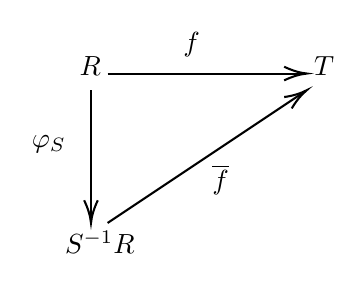
\begin{tikzpicture}[x=0.75pt,y=0.75pt,yscale=-1,xscale=1]
%uncomment if require: \path (0,476); %set diagram left start at 0, and has height of 476

%Straight Lines [id:da3152671411941921] 
\draw    (240,128) -- (334,128) ;
\draw [shift={(336,128)}, rotate = 180] [color={rgb, 255:red, 0; green, 0; blue, 0 }  ][line width=0.75]    (10.93,-3.29) .. controls (6.95,-1.4) and (3.31,-0.3) .. (0,0) .. controls (3.31,0.3) and (6.95,1.4) .. (10.93,3.29)   ;
%Straight Lines [id:da5751301154780408] 
\draw    (232,136) -- (232,198) ;
\draw [shift={(232,200)}, rotate = 270] [color={rgb, 255:red, 0; green, 0; blue, 0 }  ][line width=0.75]    (10.93,-3.29) .. controls (6.95,-1.4) and (3.31,-0.3) .. (0,0) .. controls (3.31,0.3) and (6.95,1.4) .. (10.93,3.29)   ;
%Straight Lines [id:da5543492055231241] 
\draw    (240,200) -- (334.34,137.11) ;
\draw [shift={(336,136)}, rotate = 146.31] [color={rgb, 255:red, 0; green, 0; blue, 0 }  ][line width=0.75]    (10.93,-3.29) .. controls (6.95,-1.4) and (3.31,-0.3) .. (0,0) .. controls (3.31,0.3) and (6.95,1.4) .. (10.93,3.29)   ;

% Text Node
\draw (225,118.4) node [anchor=north west][inner sep=0.75pt]    {$R$};
% Text Node
\draw (338,118.4) node [anchor=north west][inner sep=0.75pt]    {$T$};
% Text Node
\draw (202,156.4) node [anchor=north west][inner sep=0.75pt]    {$\varphi _{S}$};
% Text Node
\draw (218,202.4) node [anchor=north west][inner sep=0.75pt]    {$S^{-1} R$};
% Text Node
\draw (289,170.4) node [anchor=north west][inner sep=0.75pt]    {$\overline{f}$};
% Text Node
\draw (275,106.4) node [anchor=north west][inner sep=0.75pt]    {$f$};


\end{tikzpicture}
\end{center}
\end{note}
\begin{corollary}
Let $R$ be an integral domain considered as a subring of its quotient field $F$. If $E$ is a field and $f:R\to E$ is a monomorphism of rings, then there is a unique monomorphism of fields $\overline{f}:F\to E$ such that $\overline{f}\mid_R=f$. In particular any field $E_1$ containing $R$ contains an isomorphic copy $F_1$ of $F$ with $R\subset F_1\subset E$.
\end{corollary}
\begin{proof}
Let $S$ be the set of all nonzero elements of $R$ and apply Theorem 4.52 to $f:R\to E$. Then there is a homomorphism $\overline{f}:S^{-1}R\to E$ such that $\overline{f}\varphi_S=f$. To show that $\overline{f}$ is a monomorphism, observe that 
$$
\overline{f}\left( r_1/s_1 \right) =\overline{f}\left( r_2/s_2 \right) \Rightarrow \Rightarrow f\left( r_1s_2 \right) =f\left( r_2s_1 \right) \Rightarrow r_1s_2-r_2s_1=0,
$$
hence $r_1/s_1=r_2/s_2$, therefore $\overline{f}$ is monomorphism. Since $R$ is identified as $\varphi_S(R)$, we have $\overline{f}\mid_R=f$. The last statement is the special case when $f$ is the inclusion map.
\end{proof}
Now we deal with the ideal structure of rings of quotients.
\begin{theorem}
Let $S$ be a multiplicative subset of a commutative ring $R$.\par
(i) If $I$ is an ideal in $R$, then $S^{-1}I=\{a/s:a\in I,s\in S\}$ is an ideal in $S^{-1}R$.\par
(ii) If $J$ is another ideal in $R$, then 
\begin{small}
$$
S^{-1}\left( I+J \right) =S^{-1}I+S^{-1}J;\hspace{0.5cm}S^{-1}\left( IJ \right) =\left( S^{-1}I \right) \left( S^{-1}J \right) ;\hspace{0.5cm}S^{-1}\left( I\cap J \right) =S^{-1}I\cap S^{-1}J.
$$
\end{small}
\end{theorem}
\begin{proof}
(i) Let $r/s\in S^{-1}R$ and $a/s\in S^{-1}I$, then 
$$
\left( r/s \right) \left( a/s^{\prime} \right) =ra/ss^{\prime}\in S^{-1}I.
$$
Since $I$ is an ideal of $R$, we have $(r/s)(a/s)\in S^{-1}I$ and hence $S^{-1}I$ is an ideal of $S^{-1}R$.\par
(ii) For the first one, let $(a+b)/s\in S^{-1}(I+J)$, where $a\in I$ and $b\in J$. Then 
$$
\left( a+b \right) /s=a/s+b/s\in S^{-1}I+S^{-1}J.
$$
For the second one, let $ab/s\in S^{-1}(IJ)$, where $a\in I$ and $b\in J$. Then 
$$
ab/s=\left( as/s \right) \left( b/s \right) \in \left( S^{-1}I \right) \left( S^{-1}J \right) .
$$
The third one follows by a trivial discussion on the inclusion.
\end{proof}
\begin{note}\em
$S^{-1}I$ is called the \textbf{extension} of $I$ in $S^{-1}R$. Note that $r/s\in S^{-1}I$ need not imply that $r\in I$ since it is possible to have $a/s=r/s$ for some $a\in I$ and $r\notin I$.
\end{note}
\begin{theorem}
Let $S$ be a multiplicative subset of a commutative ring $R$ with identity and let $I$ be an ideal of $R$. Then $S^{-1}I=S^{-1}R$ if and only if $S\cap I\ne\emptyset$.
\end{theorem}
\begin{proof}
If $S\cap I\ne\emptyset$, let $s\in S\cap I$, then $s/s\in S^{-1}I$ is the identity of $S_{-1}R$, hence $S^{-1}R=S^{-1}I$. Conversely, if $S^{-1}R=S^{-1}I$, then $\varphi_S^{-1}(S^{-1}I)=R$ whence $\varphi_S(1_R)=a/s$ for some $a\in I$ and $s\in S$. Since $\varphi_S(1_R)=1_Rs/s$ we have $s^2s_1=ass_1$ for some $s_1\in S$. But $ass_1\in I$ and $s^2s_1\in S$, which shows that $S\cap I\ne\emptyset$.
\end{proof}
In order to characterize the prime ideals in a ring of quotients we need a lemma. Recall that if $J$ is an ideal in a ring of quotients $S^{-1}R$, then $\varphi_S^{-1}(J)$ is an ideal in $R$ by Exercise 4.30. We sometimes call $\varphi_S^{-1}(J)$ the \textbf{concentration} of $J$ in $R$.
\begin{lemma}\em
Let $S$ be a multiplicative subset of a commutative ring $R$ with identity and let $I$ be an ideal i $R$.\par
(i) $I\subset\varphi_S^{-1}(S^{-1}I)$.\par
(ii) If $I=\varphi_S^{-1}(J)$ for some ideal $J$ in $S^{-1}R$, then $S^{-1}I=J$. In other words ideal in $S^{-1}R$ is of the form $S^{-1}I$ for some ideal $I$ in $R$.\par
(iii) If $P$ is a prime ideal in $R$ and $S\cap P=\emptyset$, then $S^{-1}P$ is a prime ideal in $S^{-1}R$ and $\varphi_S^{-1}(P)=P$.
\end{lemma}
\begin{proof}
(i) Let $a\in I$, then by the definition of $\varphi_S$ we have $\varphi _S\left( a \right) =as/s\in S^{-1}I$, hence $I\subset\varphi_S^{-1}(S^{-1}I)$.\par
(ii) Suppose $r/s\in S^{-1}I$, then $r\in I$ and hence $\varphi_S(r)\in J$. Therefore $r/s=\left( 1_R/s \right) \left( rs/s \right) =\left( 1_R/s \right) \varphi _S\left( r \right) \in J$, hence $S^{-1}I\subset J$. Conversely, let $r/s\in J$, then $\varphi _S\left( r \right) =rs/s=\left( r/s \right) \left( ss/s \right) \in J$, hence $J\subset S^{-1}R$, therefore $S^{-1}R=J$.\par
(iii) Since $P\cap R=\emptyset$, by Theorem 4.55 we know that $S^{-1}P$ is an ideal of $S^{-1}R$, and $S^{-1}P\ne S^{-1}R$. Now we show that $S^{-1}P$ is a prime ideal of $S^{-1}R$. Suppose $(r/s)(r^\prime/s^\prime)\in S^{-1}P$, then $rr^\prime/ss^\prime=a/t\in S^{-1}P$, whence there exists some $s_1\in S$ such that $s_1trr^\prime=s_1ss^\prime t\in P$. Since $s_1t\in S$ and $S\cap P=\emptyset$, we have $rr^\prime\in P$ since $P$ is prime in $R$. Therefore neither $r\in P$ nor $r^\prime\in P$. Suppose $r\in P$, then $r/s\in S^{-1}P$, hence $S^{-1}P$ is a prime ideal of $S^{-1}R$. By (i) we have $P\subset\varphi_S^{-1}(S^{-1}P)$, now we show the converse inclusion. Let $r\in\varphi_S^{-1}(S^{-1}P)$, then $\varphi_S(r)\in S^{-1}P$. Thus $\varphi_S(r)=rs/s=a/t\in S^{-1}P$ for some $a\in P$ and $t\in S$. Therefore there exists some $s_1\in S$ such that $s_1trr^\prime=s_1ss^\prime t\in P$. Since $s_1st\in S$ and $S\cap P=\emptyset$, we have $r\in P$ since $P$ is a prime ideal of $R$. Therefore $\varphi_S^{-1}(S^{-1}P)\subset P$ and we finished our proof.
\end{proof}
\begin{theorem}
Let $S$ be a multiplicative subset of a commutative ring $R$ with identity. Then there is a one-to-one correspondence between the set $\mathcal{U}$ of prime ideals of $R$ which are disjoint from $S$ and the set $\mathcal{V}$ of prime ideals of $S^{-1}R$, given by $P\mapsto S^{-1}P$.
\end{theorem}
\begin{proof}
By Lemma 4.2(iii) we know that the mapping $P\mapsto S^{-1}P$ defines an injective map $\mathcal{U}\to\mathcal{V}$. To show that it is surjective, let $J$ be a prime ideal in $S^{-1}R$ and consider $P=\varphi_S^{-1}(J)$. By Lemma 4.2(ii) we have $S^{-1}P=J$, hence it suffices to show that $P$ is prime. Let $ab\in P$, then $\varphi_S(a)\varphi_S(b)=\varphi_S(ab)\in J$. Since $J$ is prime in $S^{-1}J$, we have $\varphi_S(a)\in J$ or $\varphi_S(b)\in J$, whence $P$ is prime.
\end{proof}
Let $R$ be a commutative ring with identity and $P$ a prime ideal of $R$. Then $S=R-P$ is a multiplicative subset of $R$. The ring of quotients $S^{-1}R$ is called the \textbf{localization} of $R$ at $P$ and is denoted by $R_P$. If $I$ is an ideal in $R$, then the ideal $S^{-1}I$ in $R_P$ is denoted $I_P$.
\begin{theorem}
Let $P$ be a prime ideal in a commutative ring $R$ with identity.\par
(i) There is a one-to-one correspondence between the set of prime ideals of $R$ which are contained in $P$ and the set of prime ideals of $R_P$, given by $Q\mapsto Q_P$;\par
(ii) The ideal $P_P$ in $R_P$ is the unique maximal ideal of $R_P$.
\end{theorem}
\begin{proof}
(i) Let $Q$ be a prime ideal contained in $P$, therefore $Q\cap S=\emptyset$, whence by Theorem 4.56 we finished our proof.\par
(ii) Let $M$ be a maximal ideal of $R_P$, since $R_P$ is a commutative ring with identity, then $M$ is prime, and hence of the form $Q_P$, where $Q$ is prime. Since $P$ is a prime ideal, we have $Q_P\subset P_P$. However by the maximal property of $M$ we have $P_P=Q_P$.
\end{proof}
Rings with a unique maximal ideal, such as $R_P$ in Theorem 4.57, are of some interest in their own right.
\begin{definition}
A \textbf{local ring} is a commutative ring with identity which has a unique maximal.
\end{definition}
\begin{note}\em
Since every ideal in a ring with identity is contained in some maximal ideal, the unique maximal ideal must contain all ideals exclude the ring itself.
\end{note}
\begin{example}\em
If $p$ is prime and $n\ge 1$, then $\mathbb{Z}_{p^n}$ is a local ring with maximal ideal $(p)$.
\end{example}
\begin{theorem}
If $R$ is a commutative ring with identity then the following conditions are equivalent.\par
(i) $R$ is a local ring;\par
(ii) all nonunits of $R$ are contained in some ideal $M\ne R$;\par
(iii) the nonunits of $R$ form an ideal.
\end{theorem}
\begin{proof}
(i)$\Rightarrow$(ii): Since $R$ is a local ring, suppose $M$ is the maximal ideal of $R$. Therefore for a nonunit $a\in R$, we have $(a)\ne R$, and hence $(a)\subset M$, therefore $a\in M$.\par
(ii)$\Rightarrow$(iii) and (iii)$\Rightarrow$(i) follows from the following fact: $I\ne R$ if and only if $I$ consists of only nonunits. If not, then suppose $I$ is an ideal of $R$ and $a\in I$, then $(a)\subset I$. Since $I\ne R$, we have $(a)\ne R$, whence $a$ is a nonunit.
\end{proof}
\begin{center}
\begin{large}
    \textbf{Exercises for 4.4}
\end{large}
\end{center}
\begin{problem}\em
Determine the complete ring of quotients of the ring $\mathbb{Z}_n$ for each $n\ge 2$.
\end{problem}
\begin{proof}
We state that every finite ring $R$ has its complete quotient ring $R$. We first state that for all $a\in R$, $a$ is either a unit or a zero divisor. Suppose $a$ is not a zero divisor, then we may define $f:b\mapsto ab$. Since $a$ is not zero divisor, it has trivial kernel. Since $|R|<\infty$, we have $f$ a bijection and hence $a$ is a unit. Now by the universal property of localization we consider the identity map $\mathrm{id}:R\to R$ factor through $S^{-1}R$:
$$
R\longrightarrow S^{-1}R\longrightarrow R,
$$
whence $R\cong S^{-1}R$. Therefore the complete ring of quotients of $\mathbb{Z}_n$ is $\mathbb{Z}_n$ itself.
\end{proof}
\begin{problem}\em
Let $S$ be a multiplicative subset of a commutative ring $R$ with identity and let $T$ be a multiplicative subset of the ring $S^{-1}R$. Let $S_*=\{r\in R:r/s\in T\ \text{for some}\ s\in S\}$, then $S_*$ is a multiplicative subset of $R$ and there is a ring isomorphism $S_*^{-1}R\cong T^{-1}(S^{-1}R)$.
\end{problem}
\begin{proof}
We first show that $S_*$ is a multiplicative subset of $R$. Let $r_1,r_2\in S_*$, then $r_1/s,r_2/s\in T$. Since $T$ is a multiplicative subset of $S^{-1}R$ we have $(r_1/s)(r_2/s)=r_1r_2/s_1s_2\in T$, and since $s_1s_2\in S$ we have $r_1r_2\in S_*$. Now define $f:r/s_*\mapsto(r/s)/(s_*/s)$, which is an isomorphism and hence $S_*^{-1}R\cong T^{-1}(S^{-1}R)$.
\end{proof}
\begin{problem}\em
(a) The set $E$ of positive even integers is a multiplicative subset of $\mathbb{Z}$ such that $E^{-1}(\mathbb{Z})$ is a field of rational numbers.\par
(b) State and prove conditions on a multiplicative subset $S$ of $\mathbb{Z}$ which insure that $S^{-1}\mathbb{Z}$ is the field of rationals.
\end{problem}
\begin{proof}
(a) Let $p/q\in\mathbb{Q}$. If $q\in E$, then $p/q\in E^{-1}\mathbb{Z}$. Otherwise consider $2p/2q$, since $E$ is the set of all even numbers we have $2p/2q\in E^{-1}\mathbb{Z}$, whence $p/q\in E^{-1}\mathbb{Z}$. Therefore $\mathbb{Q}\subset E^{-1}\mathbb{Z}$. The converse inclusion is trivial.\par
(b) Let $E$ be the set of numbers that are times of $k$, here $k\in\mathbb{Z}\setminus\{0\}$, then $E^{-1}\mathbb{Z}=\mathbb{Q}$.
\end{proof}
\begin{problem}\em
If $S=\{2,4\}$ and $R=\mathbb{Z}_6$, then $S^{-1}R$ is isomorphic to the field $\mathbb{Z}_3$.
\end{problem}
\begin{proof}
We list the all possible elements in $S^{-1}\mathbb{Z}_6$: 
$$
\frac{1}{2},\frac{2}{2},\frac{3}{2},\frac{4}{2},\frac{5}{2},\frac{6}{2},\frac{1}{4},\frac{2}{4},\frac{3}{4},\frac{4}{4},\frac{5}{4},\frac{6}{4}.
$$
Then we delete the duplicated elements we get 
$$
S^{-1}R=\left\{ \frac{2}{4},\frac{4}{4},\frac{6}{4} \right\} \cong \mathbb{Z} _3.
$$
\end{proof}
\begin{note}\em
This exercise shows that the converse of Theorem 4.50(ii) is false.
\end{note}
\begin{problem}\em
Let $R$ be an integral domain with quotient field $F$. If $T$ is an integral domain such that $R\subset T\subset F$, then $F$ is isomorphic to the quotient field $T$.
\end{problem}
\begin{proof}
First by the universal property of quotient fields we may show that the quotient fields of $T$ are isomorphic. Hence we may assume that the quotient field of $T$ is $F_T$. Therefore since $T\subset F$, we have $F_T\subset F$. For the converse inclusion, we observe that $R\subset F_T\subset F$, whence $F_T=F$ and the proof is finished.
\end{proof}
\begin{problem}\em
Let $S$ be a multiplicative subset of an integral domain $R$ such that $0\notin S$. If $R$ is a PID [resp. UFD], then so is $S^{-1}R$.
\end{problem}
\begin{proof}
For the condition that $R$ is PID, since there is a one-to-one corresponding of ideals of $R$ and $S^{-1}R$, it suffices to show that $S^{-1}I$ is a principal ideal of $S^{-1}R$, where $I$ is an ideal of $R$. Since $R$ is PID, let $I=(a)$, then $S^{-1}I=(a/s)$ for some $s\in S$, since $s\ne 0$. Therefore $S^{-1}I$ is a principal ideal of $S^{-1}R$ and hence a PID. For the condition that $R$ is UFD, we use the Kaplansky condition (Exercise 4.44). Since there is a one-to-one corresponding of ideals of $R$ and $S^{-1}R$, let $I$ be a prime ideal of $R$, and hence it contains a nonzero principal ideal that is prime, denote as $(p)$. Clearly $S^{-1}(p)$ is a nonzero principal prime ideal of $S^{-1}R$ that is contained in $S^{-1}I$, we obtain that $S^{-1}R$ is a UFD.
\end{proof}
\begin{problem}\em
Let $R_1$ and $R_2$ be integral domains with quotient fields $F_1$ and $F_2$ respectively. If $f:R_1\to R_2$ is an isomorphism, then $f$ extends to an isomorphism $F_1\cong F_2$.
\end{problem}
\begin{proof}
Let $\overline{f}:F_1\to F_2$ defined by $r/s\mapsto f(r)/f(s)$. Since $f:R_1\to R_2$ is an isomorphism, then the restriction on the set $S_1$ of all units of $R_1$ is also an isomorphism, whence $S_1\cong S_2$. Therefore $\overline{f}$ is an isomorphism, and hence $F_1\cong F_2$.
\end{proof}
\begin{problem}\em
Let $R$ be a commutative ring with identity, $I$ an ideal of $R$ and $\pi:R\to R/I$ the canonical projection.\par
(a) If $S$ is a multiplicative subset of $R$, then $\pi S=\pi(S)$ is a multiplicative subset of $R/I$;\par
(b) The mapping $\theta:S^{-1}R\to(\pi S)^{-1}(R/I)$ given by $r/s\mapsto\pi(r)/\pi(s)$ is a well-defined function.\par
(c) $\theta$ is a ring epimorphism with kernel $S^{-1}I$ and hence induces a ring isomorphism $S^{-1}R/S^{-1}I\cong(\pi S)^{-1}(R/I)$.
\end{problem}
\begin{proof}
(a) Let $s_1,s_2\in S$. Then $\pi(s_1)\pi(s_2)=(s_1I)(s_2I)=(s_1s_2I)$. Since $S$ is a multiplicative subset of $R$, then $s_1s_2\in S$, whence $\pi(s_1)\pi(s_2)\in S/I$, hence $\pi S$ is a multiplicative subset of $R/I$.\par
(b) Let $r_1/s_1=r_2/s_2$, we show that $\pi(r_1/s_1)=\pi(r_2/s_2)$. It suffices to observe that 
$$
\pi \left( s_0 \right) \left( \pi \left( a_1 \right) \pi \left( b_2 \right) -\pi \left( b_1 \right) \pi \left( a_2 \right) \right) =s_0I\left( a_1b_2I-a_2b_1I \right) =s_0\left( a_1b_2-a_2b_1 \right) I=0I=0,
$$
for some $s_0$ since $r_1/s_1=r_2/s_2$.\par
(c) We first show that $\theta$ is an epimorphism. Let $rI/\pi(s)\in(\pi S)^{-1}(R/I)$, then take $r/s\in S^{-1}R$, we obtain $\pi(r/s)=rI/\pi(s)$. Then we show that $\mathrm{Ker}\theta=S^{-1}I$. Clearly $S^{-1}I\subset\mathrm{Ker}\theta$. Conversely, if $r/s\in\mathrm{Ker}\theta$, then $\pi(r)/\pi(s)=1$, whence $r\in\mathrm{Ker}\pi$. Therefore $\mathrm{Ker}\theta\subset S^{-1}I$. Then by the First Isomorphism Theorem we obtain $S^{-1}R/S^{-1}I\cong(\pi S)^{-1}(R/I)$.
\end{proof}
\begin{problem}\em
Let $S$ be a multiplicative subset of a commutative ring $R$ with identity. If $I$ is an ideal in $R$, then $S^{-1}(\mathrm{Rad}I)=\mathrm{Rad}(S^{-1}I)$.
\end{problem}
\begin{proof}
Let $a/b\in S^{-1}(\mathrm{Rad}I)$. Then $a\in\mathrm{Rad}I$, and hence there exists some $n$ such that $a^n\in I$. Since $S$ is a multiplicative subset of $R$, we have $a^n/b^n=(a/b)^n\in S^{-1}I$, whence $a/b\in\mathrm{Rad}(S^{-1}I)$. For the inverse inclusion, let $a/b\in\mathrm{Rad}(S^{-1}I)$. Then for some $n$ we have $(a/b)^n=a^n/b^n\in S^{-1}I$. Therefore $a^n\in I$ for some $I$ and hence $a\in\mathrm{Rad}I$. This implies $a/b\in S^{-1}\mathrm{Rad}I$.
\end{proof}
\begin{problem}\em
Let $R$ be an integral domain and for each maximum ideal $M$, consider $R_M$ as a subring of the quotient field of $R$. Let $\mathcal{M}$ be the collection of all maximal ideals of $R$, show that $\bigcap_{M\in\mathcal{M}}R_M=R$.
\end{problem}
\begin{proof}
Let $r/s\in\bigcap_{M\in\mathcal{M}}R_M$, then $r/s\in S^{-1}R$, where $s\in R-M$ for all $M\in\mathcal{M}$. Therefore for all $M\in\mathcal{M}$ we have $s\notin M$, whence $(s)\not\subset M$. This is true if and only if $s=1$, whence $r/s\in R$. The converse condition is trivial.
\end{proof}
\begin{problem}\em
A commutative ring with identity is local if and only if for all $r,s\in R$, $r+s=1_R$ implies $r$ or $s$ is a unit.
\end{problem}
\begin{proof}
If $R$ is a commutative ring with identity and is a local ring, let $r,s\in R$ and $r+s=1_R$. Then if $r$ and $s$ are both nonunit, we have $r,s\in M$, where $M$ is the maximal ideal of $R$. Therefore $r+s\in M$, and hence $1_R\in M$, which is a contradiction! Conversely, if $r+s=1_R$ and either $r$ or $s$ is a unit, then we show that every nonunit $a$ is contained in a chosen maximal ideal $M$ of $R$. If not, let $x$ is a nonunit and $xR+M=R$. Let $xr+m=1$, then $m=1-xr\in M$, a contradiction!
\end{proof}
\begin{problem}\em
The ring $R$ consisting of all rational numbers with denominators not divisible by some (fixed) prime $p$ is a local ring.
\end{problem}
\begin{proof}
Observe that the ring $R$ here is the localization $\mathbb{Z}_{(p)}$ of the integers $\mathbb{Z}$ at the prime ideal $(p)$, whence is a local ring.
\end{proof}
\begin{problem}\em
If $M$ is a maximal ideal in a commutative ring $R$ with identity and $n$ is a positive integer, then the ring $R/M^n$ has a unique prime ideal and therefore is local.
\end{problem}
\begin{proof}
If $n=1$, then the condition is trivial. For $n\ge 2$, recall that the ideal of $R/M^n$ corresponds to the ideal of $R$ which contains $M^n$, therefore let $I$ be an ideal of $R$ contains $M^n$, then it contains $M$. However $M$ is the maximal ideal of $R$, therefore $I=M$, and hence the ideal corresponds to the one of $R/M^n$ is $M/M^n$, which is unique and hence local.
\end{proof}
\begin{problem}\em
Every nonzero homomorphic image of a local ring is local.
\end{problem}
\begin{proof}
Let $R$ be a local ring and $S$ be a ring with homomorphism $f:R\to S$. Then by the first isomorphism theorem we have $\mathrm{Im}f\cong R/\mathrm{Ker}f$. Since the ideals of $R$ and $R/\mathrm{Ker}f$ corresponds to each other, if $R$ has a maximal ideal, so is $R/\mathrm{Ker}f$. Therefore $\mathrm{Im}f$ must contain a maximal ideal, whence local.
\end{proof}
\subsection{Rings of Polynomials and Formal Power Series}
We begin by defining and developing notation for polynomials in one indeterminate over a ring $R$. Next the ring of polynomials in $n$ indeterminates over $R$ is defined and its basic properties are developed. The last part of this section is a brief introduction to the ring of formal power series in one indeterminate over $R$.
\begin{theorem}
Let $R$ be a ring and let $R[x]$ denote the set of all sequences of elements of $R(a_0,a_1,\cdots)$ such that $a_i=0$ for all but a finite number of indices $i$.\par
(i) $R[x]$ is a ring with addition and multiplication defined by 
$$
\left( a_0,a_1,\cdots \right) +\left( b_0,b_1,\cdots \right) =\left( a_0+b_0,a_1+b_1,\cdots \right) 
$$
and multiplication 
$$
\left( a_0,a_1,\cdots \right) \left( b_0,b_1,\cdots \right) =\left( c_0,c_1,\cdots \right) ,c_n=\sum_{i+j=n}{a_ib_j}=\sum_{k=0}^n{a_kb_{n-k}}.
$$\par
(ii) If $R$ is commutative [resp. a ring with identity or a ring with no zero divisors or an integral domain], then so is $R[x]$.\par
(iii) The map $R\to R[x]$ given by $r\mapsto(r,0,\cdots)$ is a monomorphism.
\end{theorem}
\begin{proof}
(i) We only check the second and the third multiplicative laws of $R[x]$, while the rest part is trivial. It suffices to observe that 
$$
\sum_{i+j=n}{d_ic_j}=\sum_{i+j=n}{\sum_{k+l=i}{a_kb_lc_j}}=\sum_{\left( n-k \right) +k=n}{\sum_{l+j=n-k}{a_kb_lc_j}}
$$
and 
$$
\sum_{i+j=n}{a_i\left( b_j+c_j \right)}=\sum_{i+j=n}{a_ib_j}+\sum_{i+j=n}{a_ic_j}.
$$\par
(ii) We only show the condition that $R$ is commutative and the rest part may be proved by definition analogously. Suppose $R$ is commutative, then 
$$
\sum_{i+j=n}{a_ib_j}=\sum_{i+j=n}{b_ia_j},
$$
which finished the proof.\par
(iii) Trivial. One may verify this by definition.
\end{proof}
The ring $R[x]$ in Theorem 4.60 is called the \textbf{ring of polynomials} over $R$. Its elements are called \textbf{polynomials}. We now develop a familiar notation for polynomials.
\begin{theorem}
Let $R$ be a ring with identity and denote by $x$ the element $(0,1_R,0,\cdots)$ of $R[x]$.\par
(i) $x^n=(0,\cdots,0,1_R,0,\cdots)$, where $1_R$ is the $n+1$st coordinate.\par
(ii) If $r\in R$, then for each $n\ge 0$, $rx^n=x^nr=(0,\cdots,0,r,0,\cdots)$, where $r$ is the $n+1$st coordinate.\par
(iii) For every nonzero polynomial $f\in R[x]$ there exists an integer $n\in\mathbb{N}$ and elements $a_0,a_1,\cdots,a_n\in R$ such that $f=a_0x^0+a_1x^1+\cdots+a_nx^n$. The integer $n$ and elements $a_i$ are unique in the sense that $f=b_0x^0+b_1x^1+\cdots+b_mx^m$ implies $m\ge n$, $a_i=b_i$ for $i=1,2,\cdots,n$ and $b_i=0$ for $n<i\le m$.
\end{theorem}
\begin{proof}
(i) and (ii) follows from trivial calculations. For (iii), observe that if $(a_0,a_1,\cdots,a_n)\in R[x]$, then $f=a_0x^0+a_1x^1+\cdots+a_nx^n$ is the desired result.
\end{proof}
If $R$ has an identity, then $x^0=1_R$ (as in the ring with identity) and we write the polynomial $f=a_0x^0+a_1x^1+\cdots+a_nx^n$ as $f=a_0+a_1x+\cdots+a_nx^n$. If $R$ has no identity, then $R$ may be embedded into a ring $S$ with identity by Theorem 4.10, whence $R[x]$ may be seen as the subring of $S[x]$, and hence every element in $R[x]$ may be written as $f=a_0+a_1x+\cdots+a_nx^n$, where $a_i\in S$.\par
Hereafter a polynomial $f$ over a ring $R$ (with or without identity) will always be written in the form $f=a_0+a_1x+\cdots+a_nx^n$, where $a_i\in R$. In this notation addition and multiplication in $R[x]$ are given by the familiar rules: 
$$
\sum_{i=0}^n{a_ix^i}+\sum_{i=0}^n{b_ix^i}=\sum_{i=0}^n{\left( a_i+b_i \right) x^i},\left( \sum_{i=0}^n{a_ix^i} \right) \left( \sum_{i=0}^n{b_ix^i} \right) =\sum_{k=0}^{m+n}{\sum_{i+j=k}{a_ib_jx^k}}.
$$
If $f=\sum_{i=0}^na_ix^i\in R[x]$, then the elements $a_i\in R$ are called the \textbf{coefficients} of $f$. The element $a_0$ is called the \textbf{constant term}. Elements of $R$, which all have the form $r=(r,0,\cdots)=rx^0$ are called \textbf{constant polynomials}. If $f=\sum_{i=0}^na_ix^i$, then $a_n$ is called the \textbf{leading coefficient} of $f$. If $R$ has an identity and leading coefficient $1_R$, then $f$ is said to be the \textbf{monic polynomial}.\par
Let $R$ be a ring (with identity). For historical reasons the element $x=(0,1_R,0,\cdots)$ of $R[x]$ is called an \textbf{indeterminate}. One speaks of polynomials in the indeterminate $x$. If $S$ is another ring (with identity), then the indeterminate $x\in S[x]$ is not the same element as $x\in R[x]$. In context this ambiguous notation will cause no confusion.\par
If $R$ is any ring, it is sometimes convenient to distinguish one copy of the polynomial ring over $R$ from another. In this situation the indeterminate in one copy is denoted by one symbol, say $x$, and another is denoted by another symbol, say $y$. In the latter case the polynomial ring is denoted $R[y]$.\par
We shall now define polynomials in more than one indeterminate. The definition is motivated by the following fact: every polynomial in one indeterminate is by definition a particular kind of sequence, that is, a function $\mathbb{N}\to R$. For instance, $(a_0,a_1,\cdots,a_n)$ is a function such that $i\mapsto a_i$. Therefore for each integer $n$ let $\mathbb{N}^n=\mathbb{N}\times\mathbb{N}\times\cdots\times\mathbb{N}$. The elements of $\mathbb{N}^n$ are ordered $n$ tuples of elements of $\mathbb{N}$. $\mathbb{N}^n$ is clearly an additive abelian monoid under coordinate-wise addition.
\begin{theorem}
Let $R$ be a ring and denote $R[x_1,\cdots,x_n]$ the set of all functions $f:\mathbb{N}^n\to R$ such that $f(u)\ne 0$ for at most a finite number of elements $u$ of $\mathbb{N}^n$.\par
(i) $R[x_1,\cdots,x_n]$ is a ring with addition and multiplication defined by 
$$
\left( f+g \right) \left( u \right) =f\left( u \right) +g\left( u \right) ,\left( fg \right) \left( u \right) =\sum_{v+w=u;v,w\in \mathbb{N} ^n}{f\left( v \right) g\left( w \right)},
$$
where $f,g\in R[x_1,\cdots,x_n]$ and $u\in\mathbb{N}^n$.\par
(ii) If $R$ is commutative [resp. a ring with identity or a ring without zero divisors or an integral domain], then so is $R[x_1,\cdots,x_n]$.\par
(iii) The map $R\to R[x_1,\cdots,x_n]$ given by $r\mapsto f_r$, where $f_r(0,\cdots,0)=r$ and $f(u)=0$ for all other $u\in\mathbb{N}^n$, is a monomorphism of rings.
\end{theorem}
\begin{proof}
(i) We only show that the second multiplicative law of a ring is satisfied, which suffices to observe 
$$
\begin{aligned}
\left( fg \right) h\left( u \right) &=\sum_{v+w=u;v,w\in \mathbb{N} ^n}{\left( fg \right) \left( v \right) h\left( w \right)}=\sum_{v+w=u;v,w\in \mathbb{N} ^n}{\sum_{p+q=v;p,q\in \mathbb{N} ^n}{f\left( p \right) g\left( q \right) h\left( w \right)}}
\\
&=\sum_{\left( u-p \right) +p=u;u-p,p\in \mathbb{N} ^n}{\sum_{q+w=u-p;q,w\in \mathbb{N} ^n}{f\left( p \right) g\left( q \right) h\left( w \right)}}=f\left( gh \right) \left( u \right) .
\end{aligned}
$$\par
(ii) We only proof the condition when $R$ is a commutative ring. Then 
$$
\left( fg \right) \left( u \right) =\sum_{v+w=u;v,w\in \mathbb{N} ^n}{f\left( v \right) g\left( w \right)}=\sum_{v+w=u;v,w\in \mathbb{N} ^n}{g\left( w \right) f\left( v \right)}=\left( gf \right) \left( u \right) 
$$
for all $u\in\mathbb{N}^n$, whence $fg=gf$.\par
(iii) This is trivial by definition.
\end{proof}
The ring $R[x_1,\cdots,x_n]$ of Theorem 4.62 is called the \textbf{ring of polynomials in $n$ indeterminates} over $R$. $R$ is identified with its isomorphic image under the map of Theorem 4.62(iii) and considered as a subring of $R[x_1,\cdots,x_n]$. If $n=1$, then $R[x_1]$ is precisely the ring of polynomials with one indeterminates as stated in Theorem 4.60. Let $\varepsilon_i=(0,\cdots,1,\cdots,0)$, where $1$ at the $i$th coordinate of $\varepsilon_i$, then every element in $\mathbb{N}^n$ may be written in the form of $k_1\varepsilon_1+\cdots+k_n\varepsilon_n$.\par
The following theorem states some basic properties of elements of $R[x_1,\cdots,x_n]$. Note that the ring $R[x_1,\cdots,x_n]$ here being discussed are of finite indeterminates, and the general case is left as an exercise.
\begin{theorem}
Let $R$ be a ring with identity and $n$ a positive integer. For each $i=1,2,\cdots,n$ let $x_i\in R[x_1,\cdots,x_n]$ be defined by $x_i(\varepsilon_i)=1_R$ and $x_i(u)=0$ for $u\ne\varepsilon_i$.\par
(i) For each integer $k\in\mathbb{N}$, $x_i^k(k\varepsilon_i)=1_R$ and $x_i^k(u)=0$ for $u\ne k\varepsilon_i$.\par
(ii) For each $(k_1,k_2,\cdots,k_n)\in\mathbb{N}^n$, $x_{1}^{k_1}x_{2}^{k_2}\cdots x_{n}^{k_n}\left( k_1\varepsilon _1+k_2\varepsilon _2+\cdots +k_n\varepsilon _n \right) =1_R$ and $x_{1}^{k_1}x_{2}^{k_2}\cdots x_{n}^{k_n}\left( u \right) =0$ for $u\ne k_1\varepsilon_1+k_2\varepsilon_2+\cdots+k_n\varepsilon_n$.\par
(iii) $x_{i}^{s}x_{j}^{t}=x_{j}^{t}x_{i}^{s}$ for all $s,t\in\mathbb{N}$ and all $i=1,2,\cdots,n$.\par
(iv) $x_i^tr=rx_i^t$ for all $r\in R$ and all $t\in\mathbb{N}$.\par
(v) For every polynomial $f\in R[x_1,\cdots,x_n]$ there exist unique $a_{k_1,\cdots,k_n}\in R$, indexed by all $(k_1,\cdots,k_n)\in\mathbb{N}^n$ and nonzero for all at most a finite number of $(k_1,\cdots,k_n)\in\mathbb{N}^n$, such that 
$$
f=\sum_{\left( k_1,k_2,\cdots ,k_n \right) \in \mathbb{N} ^n}{a_{k_1,\cdots,k_n}x_{1}^{k_1}x_{2}^{k_2}\cdots x_{n}^{k_n}}.
$$
\end{theorem}
\begin{proof}
(i) It suffices to observe 
$$
x_{i}^{k}\left( k\varepsilon _i \right) =\sum_{u_1+\cdots +u_k=k\varepsilon _i}{x_i\left( u_1 \right) \cdots x_i\left( u_k \right)}=x_i\left( \varepsilon _i \right) \cdots x_i\left( \varepsilon _i \right) =1_R
$$
and 
$$
x_{i}^{k}\left( u \right) =\sum_{u_1+\cdots +u_k=u}{x_i\left( u_1 \right) \cdots x_i\left( u_k \right)}=0
$$
since it is impossible for all $u_i=\varepsilon_i$ when $u\ne k\varepsilon_i$, and hence there exists at least one $x_i(u_j)=0$.\par
(ii) By definition of multiplication we have 
$$
\begin{aligned}
&x_{1}^{k_1}x_{2}^{k_2}\cdots x_{n}^{k_n}\left( k_1\varepsilon _1+k_2\varepsilon _2+\cdots +k_n\varepsilon _n \right) 
\\
&=\sum_{u_1+\cdots +u_n=u}{\left[ \sum_{v_{1}^{\left( 1 \right)}+\cdots +v_{k_1}^{\left( 1 \right)}=u_1}{\cdots \sum_{v_{1}^{\left( n \right)}+\cdots +v_{k_n}^{\left( n \right)}=u_n}{\left( \prod_{i=1}^{k_1}{x_1\left( v_{i}^{\left( 1 \right)} \right)}\cdots \prod_{i=1}^{k_n}{x_n\left( v_{i}^{\left( n \right)} \right)} \right)}} \right]}
\\
&=\prod_{i=1}^{k_1}{x_1\left( \varepsilon _1 \right)}\prod_{i=1}^{k_2}{x_1\left( \varepsilon _2 \right)}\cdots \prod_{i=1}^{k_n}{x_n\left( \varepsilon _n \right)}=1_R,
\end{aligned}
$$
and $x_{1}^{k_1}x_{2}^{k_2}\cdots x_{n}^{k_n}\left( u \right) =0$ for $u\ne k_1\varepsilon_1+k_2\varepsilon_2+\cdots+k_n\varepsilon_n$.\par
(iii) Observe that 
\begin{small}
$$
\begin{aligned}
x_{i}^{s}x_{j}^{t}\left( u \right) =\sum_{u_1+u_2=u}{x_{i}^{s}\left( u_1 \right) x_{i}^{s}\left( u_2 \right)}&=\sum_{u_1+u_2=u}{\sum_{v_{1}^{\left( 1 \right)}+\cdots +v_{s}^{\left( 1 \right)}=u_1}{\sum_{v_{1}^{\left( 2 \right)}+\cdots +v_{t}^{\left( 2 \right)}=u_2}{\prod_{j=1}^s{x_i\left( v_{j}^{\left( 1 \right)} \right)}\prod_{k=1}^t{x_i\left( v_{k}^{\left( 2 \right)} \right)}}}}
\\
&=\sum_{u_1+u_2=u}{\sum_{v_{1}^{*}+\cdots +v_{s}^{*}=u}{\prod_{j=1}^t{x_i\left( v_{j}^{*} \right)}\prod_{k=t+1}^{s+t}{x_i\left( v_{k}^{*} \right)}}}=x_j^tx_i^s(u).
\end{aligned}
$$
\end{small}
hence we have $x_{i}^{s}x_{j}^{t}=x_{j}^{t}x_{i}^{s}$ for all $s,t\in\mathbb{N}$ and all $i=1,2,\cdots,n$.\par
(iv) This can be verified via definition. We skip the details.\par
(v) Let $a_{k_1,\cdots ,k_n}=f\left( k_1,\cdots ,k_n \right) $.
\end{proof}
If $R$ is a ring with identity, then the elements $x_1,\cdots,x_n\in R[x_1,\cdots,x_n]$ are called the \textbf{indeterminates}. The elements $a_0,\cdots,a_m$ in Theorem 4.63(v) are called the \textbf{coefficients} of the polynomial $f$. A polynomial of the form $ax_1^{k_1}\cdots x_n^{k_n}$ us called a \textbf{monomial} in $x_1,\cdots,x_n$. Theorem 4.63(v) shows that each polynomial is a sum of monomials. It is customary to omit those $x_i$ appear with exponent zero in a monomial. The terminologies above is extended to the ring $R[x_1,\cdots,x_n]$ in Theorem 4.63, and if $R$ has no identity, we may embed $R[x_1,\cdots,x_n]$ into $S[x_1,\cdots,x_n]$, where $S$ is a ring with identity.\par
If $R$ is a ring, then the map $R[x_1]\to R[x_1,\cdots,x_n]$ given by $\sum_{i=0}^ma_ix_1^i\mapsto\sum_{i=0}^ma_ix_1^ix_2^0\cdots x_n^0$ is easily seen to be a monomorphism of rings. Similarly, for every subset of $\{1,2,\cdots,n\}$, say $\{i_1,\cdots,i_k\}$, there is a monomorphism $R[x_{i_1},\cdots,x_{i_k}]\to R[x_1,\cdots,x_n]$. $R[x_{i_1},\cdots,x_{i_k}]$ is usually seen as its isomorphic image and considered as the subring of $R[x_1,\cdots,x_n]$.\par
Let $\varphi:R\to S$ be a homomorphism of rings, $f\in R[x_1,\cdots,x_n]$ and $s_1,\cdots,s_n\in S$. By Theorem 4.63 we have $f=\sum_{i=0}^ma_ix_1^{k_{i1}}x_2^{k_{i2}}\cdots x_n^{k_{in}}$, where $k_{ij}\in\mathbb{N}$ and $a_i\in R$. Then $\varphi f(a_1,\cdots,a_n)$ is defined to be $\sum_{i=0}^m\varphi(a_i)s_1^{k_{i1}}s_2^{k_{i2}}\cdots s_n^{k_{in}}$, which is obtained by substituting $a_i$ to $\varphi(a_i)$ and $x_i$ to $s_i$. Since $a_i$ and $k_{ij}$ are uniquely determined, $\varphi f$ is well-defined. If $R$ is a subring of $S$ and $\varphi$ is the inclusion map, then $\varphi f(x_1,\cdots,x_n)$ is written as $f(s_1,\cdots,s_n)$.\par
As is the case with most interesting algebraic constructions, the polynomial ring $R[x_1,\cdots,x_n]$ can be characterized by a universal mapping property. The following Theorem and its corollaries are true in the noncommutative case if appropriate hypotheses are added. They are also true for rings of polynomials in an infinite number of indeterminates, which we do not discuss here.
\begin{theorem}
Let $R$ and $S$ be commutative rings with identity and $\varphi:R\to S$ a homomorphism of rings such that $\varphi(1_R)=1_S$. If $s_1,\cdots,s_n\in S$, then there is a unique homomorphism of rings $\overline{\varphi}:R[x_1,\cdots,x_n]\to S$ such that $\overline{\varphi}\mid_R=\varphi$ and $\overline{\varphi}(x_i)=s_i$ for $i=1,2,\cdots,n$. This property completely determines the polynomial ring $R[x_1,\cdots,x_n]$ up to isomorphism.
\end{theorem}
\begin{proof}
Let $\overline{\varphi}$ be the mapping $f(x_1,\cdots,x_n)\mapsto\varphi f(s_1,\cdots,s_n)$, then it is easily verified that it satisfies the conditions. Now we show that $\overline{\varphi}$ is a homomorphism. Observe that 
$$
\begin{aligned}
\overline{\varphi }\left( f+g \right) &=\varphi \left[ f\left( x_1,x_2,\cdots x_n \right) +g\left( x_1,x_2,\cdots ,x_n \right) \right] =\sum_{i=0}^m{\varphi \left( a+b \right) \varphi ^{k_{i1}}\left( x_1 \right) \cdots \varphi ^{k_{n1}}\left( x_n \right)}
\\
&=\sum_{i=0}^m{\varphi \left( a \right) \varphi ^{k_{i1}}\left( x_1 \right) \cdots \varphi ^{k_{n1}}\left( x_n \right)}+\sum_{i=0}^m{\varphi \left( b \right) \varphi ^{k_{i1}}\left( x_1 \right) \cdots \varphi ^{k_{n1}}\left( x_n \right)}=\overline{\varphi }\left( f \right) +\overline{\varphi }\left( g \right) 
\end{aligned}
$$
and 
$$
\begin{aligned}
\overline{\varphi }\left( fg \right) \left( u \right) &=\overline{\varphi }\left( \sum_{v+w=u}{f\left( v \right) g\left( w \right)} \right) =\sum_{v+w=u}{\varphi f\left( v \right) \cdot \varphi g\left( w \right)}
\\
&=\sum_{v+w=u}{\left[ \sum_{i=0}^m{\varphi \left( a \right) \varphi ^{k_{i1}}\left( x_1 \right) \cdots \varphi ^{k_{n1}}\left( x_n \right) \left( v \right)}\cdot \sum_{i=0}^m{\varphi \left( b \right) \varphi ^{k_{i1}}\left( x_1 \right) \cdots \varphi ^{k_{n1}}\left( x_n \right) \left( w \right)} \right]}
\\
&=\sum_{i=0}^m{\varphi \left( a \right) \varphi ^{k_{i1}}\left( x_1 \right) \cdots \varphi ^{k_{n1}}\left( x_n \right) \left( u \right)}\cdot \sum_{i=0}^m{\varphi \left( b \right) \varphi ^{k_{i1}}\left( x_1 \right) \cdots \varphi ^{k_{n1}}\left( x_n \right) \left( u \right)}
\\
&=\overline{\varphi }\left( f \right) \left( u \right) \cdot \overline{\varphi }\left( g \right) \left( u \right) ,
\end{aligned}
$$
this showed the existence. Now suppose $\overline{\psi}$ is another homomorphism that satisfies these conditions, then 
$$
\overline{\psi }\left( f \right) =\sum_{i=0}^m{\psi \left( a \right) \psi ^{k_{i1}}\left( x_i \right) \cdots \psi ^{k_{in}}\left( x_i \right)}=\sum_{i=0}^m{\varphi \left( a \right) s_{1}^{k_{i1}}\cdots s_{n}^{k_{in}}}=\varphi f\left( s_1,\cdots ,s_n \right) ,
$$
whence $\overline{\varphi}$ is unique. By Theorem 2.61 we may show that the polynomial ring $R[x_1,\cdots,x_n]$ may be determined by this property up to isomorphism.
\end{proof}
This theorem may be repharsed into the commutative diagram as follows: 
\begin{center}


\tikzset{every picture/.style={line width=0.75pt}} %set default line width to 0.75pt        

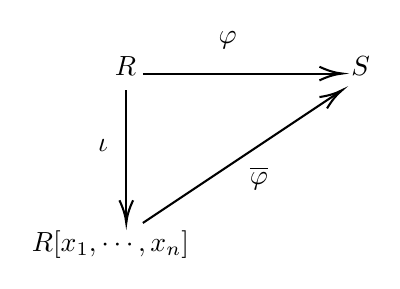
\begin{tikzpicture}[x=0.75pt,y=0.75pt,yscale=-1,xscale=1]
%uncomment if require: \path (0,476); %set diagram left start at 0, and has height of 476

%Straight Lines [id:da3152671411941921] 
\draw    (240,128) -- (334,128) ;
\draw [shift={(336,128)}, rotate = 180] [color={rgb, 255:red, 0; green, 0; blue, 0 }  ][line width=0.75]    (10.93,-3.29) .. controls (6.95,-1.4) and (3.31,-0.3) .. (0,0) .. controls (3.31,0.3) and (6.95,1.4) .. (10.93,3.29)   ;
%Straight Lines [id:da5751301154780408] 
\draw    (232,136) -- (232,198) ;
\draw [shift={(232,200)}, rotate = 270] [color={rgb, 255:red, 0; green, 0; blue, 0 }  ][line width=0.75]    (10.93,-3.29) .. controls (6.95,-1.4) and (3.31,-0.3) .. (0,0) .. controls (3.31,0.3) and (6.95,1.4) .. (10.93,3.29)   ;
%Straight Lines [id:da5543492055231241] 
\draw    (240,200) -- (334.34,137.11) ;
\draw [shift={(336,136)}, rotate = 146.31] [color={rgb, 255:red, 0; green, 0; blue, 0 }  ][line width=0.75]    (10.93,-3.29) .. controls (6.95,-1.4) and (3.31,-0.3) .. (0,0) .. controls (3.31,0.3) and (6.95,1.4) .. (10.93,3.29)   ;

% Text Node
\draw (225,118.4) node [anchor=north west][inner sep=0.75pt]    {$R$};
% Text Node
\draw (339,118.4) node [anchor=north west][inner sep=0.75pt]    {$S$};
% Text Node
\draw (217,158.4) node [anchor=north west][inner sep=0.75pt]    {$\iota $};
% Text Node
\draw (185,202.4) node [anchor=north west][inner sep=0.75pt]    {$R[ x_{1} ,\cdots ,x_{n}]$};
% Text Node
\draw (290,171.4) node [anchor=north west][inner sep=0.75pt]    {$\overline{\varphi }$};
% Text Node
\draw (275,106.4) node [anchor=north west][inner sep=0.75pt]    {$\varphi $};


\end{tikzpicture}
\end{center}
\begin{note}\em
Note that the map $R[x_1,\cdots,x_n]\to S$ given by $f\mapsto\varphi f(s_1,\cdots,s_n)$ is a homomorphism of rings even when $R$ and $S$ do not have identities.
\end{note}
A consequence of Theorem 4.64 may be illustrated by the following example. 
Let $R$ be a commutative ring and consider 
$$
f=x^2y+x^3y+x^4+xy+y^3+r\in R\left[ x,y \right] .
$$
Observe that 
$$
f=y^2+\left( x^3+x^2+x \right) y+\left( x^4+r \right) \in R\left[ x \right] \left[ y \right] ,f=x^4+yx^3+yx^2+yx+\left( y^2+r \right) \in R\left[ y,x \right] ,
$$
this suggests $R[x][y]\cong R[y][x]$. More generally, we have the following theorem: 
\begin{theorem}
Let $R$ be a commutative ring with identity and $n$ a positive integer. For each $1\le k<n$ there are isomorphisms of rings: 
$$
R\left[ x_1,\cdots ,x_k \right] \left[ x_{k+1},\cdots ,x_n \right] \cong R\left[ x_1,\cdots ,x_n \right] \cong R\left[ x_{k+1},\cdots x_n \right] \left[ x_1,\cdots ,x_k \right] .
$$
\end{theorem}
\begin{proof}
We use the universal properties to prove this statement. Let $\varphi:R\to S$ be an homomorphism of commutative rings with identity, then by Theorem 4.64 there exists $\overline{\varphi}:R[x_1,\cdots,x_n]\to S$ such that $\overline{\varphi}\mid_R=\varphi$ and $\overline{\varphi}(x_i)=s_i$ for all $1\le i\le n$. Now substitute $R$ with $R[x_1,\cdots,x_k]$ in $\varphi$ and obtain $\overline{\overline{\varphi}}:R[x_1,\cdots,x_k][x_{k+1},\cdots,x_n]\to S$ such that $\overline{\overline{\varphi}}\mid_R=\varphi$ and $\overline{\overline{\varphi}}(x_i)=s_i$ for $k+1\le i\le n$. Since $R[x_1,\cdots,x_n]$ is determined up to isomorphism by the universal property, we have $R\left[ x_1,\cdots ,x_k \right] \left[ x_{k+1},\cdots ,x_n \right] \cong R\left[ x_1,\cdots ,x_n \right] $. Similarly we may prove that $R\left[ x_{k+1},\cdots x_n \right] \left[ x_1,\cdots ,x_k \right] \cong R\left[ x_1,\cdots ,x_n \right] $.
\end{proof}
Since $R[x_1,\cdots,x_k]$ is considered as a subring of $R[x_1,\cdots,x_n]$, it is customary to identify the various polynomial rings under the isomorphisms stated in Theorem 4.65 and write $R[x_1,\cdots,x_k][x_{k+1},\cdots,x_n]=R[x_1,\cdots,x_n]$.\par
We now discuss the rings of formal power series.
\begin{theorem}
Let $R$ be a ring and denote by $R[[x]]$ the set of all sequences of elements of $R(a_0,a_1,\cdots)$.\par
(i) $R[[x]]$ is a ring with addition and multiplication defined by 
$$
\left( a_0,a_1,\cdots \right) +\left( b_0,b_1,\cdots \right) =\left( a_0+b_0,a_1+b_1,\cdots \right) 
$$
and 
$$
\left( a_0,a_1,\cdots \right) \left( b_0,b_1,\cdots \right) =\left( c_0,c_1,\cdots \right) ,c_n=\sum_{i+j=n}{a_ib_j},n=0,1,\cdots .
$$\par
(ii) The polynomial ring $R[x]$ is a subring of $R[[x]]$.\par
(iii) If $R$ is a commutative [resp. a ring with identity or a ring with no zero divisors or an integral domain], then so is $R[[x]]$.
\end{theorem}
\begin{proof}
(i) and (iii) are similar to the proof of Theorem 4.60. For (ii), consider the monomorphism $(a_0,a_1,\cdots,a_n)\mapsto(a_0,\cdots,a_n,0,\cdots)$.
\end{proof}
The ring $R[[x]]$ of Theorem 4.66 is called the \textbf{ring of formal power series} over the ring $R$. Its elements are called power series. If $R$ has an identity then the polynomial $x=(0,1_R,0,\cdots)\in R[[x]]$ is called an indeterminate. We shall also denote $(a_0,a_1,\cdots)\in R[[x]]$ as $\sum_{i=0}^\infty a_ix^i$, where $a_i$ are called \textbf{coefficients} and $a_0$ is called the constant term. This notation is also used when $R$ has no identity, with same reason to that of polynomials.
\begin{proposition}
Let $R$ be a ring with identity and $f=\sum_{i=0}^\infty a_ix^i\in R[[x]]$.\par
(i) $f$ is a unit in $R[[x]]$ if and only if its constant term $a_0$ is a unit in $R$.\par
(ii) If $a_0$ is irreducible in $R$, then $f$ is irreducible in $R[[x]]$.
\end{proposition}
\begin{proof}
(i) Suppose $f\in R[[x]]$ is a unit, then there exists some $g=\sum b_nx^n$ such that $fg=gf=1_R$. It follows immediately that $a_0b_0=b_0a_0=1_R$, whence $a_0$ is a unit in $R$. Conversely, it suffices to solve the equation below: 
$$
\begin{cases}
	a_0b_0=1_R,\\
	a_0b_1+a_1b_0=0,\\
	\vdots\\
	a_0b_n+a_1b_{n-1}+\cdots +a_nb_0=0,\\
	\vdots\\
\end{cases}
$$
Since $a_0$ is a unit, we have $b_0=a_0^{-1}$. Proceed inductively, we have $$b_n=a_{0}^{-1}\left( -a_1b_{n-1}-\cdots -a_nb_0 \right) ,$$
whence $g=\sum b_nx^n\in R[[x]]$ satisfies $fg=1_R$. Similarly we may find $h\in R[[x]]$ such that $hf=1_R$. However $h=h1_R=h(fg)=(hf)g=g$, therefore $fg=gf=1_R$ and the proof is finished.\par
(ii) follows directly from (i).
\end{proof}
\begin{corollary}
If $R$ is a division ring, then the units in $R[[x]]$ are precisely those power series with nonzero constant term. The principal ideal $(x)$ consists precisely of the nonunits in $R[[x]]$ and is the unique maximal ideal of $R[[x]]$. Thus if $R$ is a field, $R[[x]]$ is a local ring.
\end{corollary}
\begin{proof}
The first statement follows since $R$ is a division ring and Proposition 4.67 (i), since every nonzero element in a division ring is a unit. Since $x$ is in the center of $R[[x]]$, by Theorem 4.15 we have $(x)=\{xf:f\in R[[x]]\}$. Consequently, every element $xf$ of $(x)$ has zero constant term, whence $xf$ is a nonunit. Conversely every nonunit $f\in R[[x]]$ is necessarily of the form $f=\sum a_ix^i$ with $a_0=0$. Let $g=\sum b_ix^i$ where $b_i=a_{i+1}$ for all $i$. Then $xg=f$, whence $f\in (x)$. Therefore $(x)$ is the set of nonunits. Finally, since $1_R\notin(x)$, $(x)\ne R[[x]]$. Furthermore, every ideal $I$ of $R[[x]]$ with $I\ne R[[x]]$ necessarily consists of nonunits. Thus every ideal of $R[[x]]$ except $R[[x]]$ is contained in $(x)$. Therefore $R[[x]]$ is local.
\end{proof}
Some basic concepts, such as the degree of a polynomial, or the division algorithm has been introduced in the course of Linear Algebra, for which a reader may refer to any textbook of Advanced algebra, or Linear algebra. We mention an important result here: 
\begin{theorem}
If $D$ is a unique factorization domain, then so is the polynomial ring $D[x_1,\cdots,x_n]$.
\end{theorem}
We skip the proof of this result. A reader who wishes to scan the proof of this theorem may refer to GTM73 page 164. Note that a field $F$ is trivially a UFD, therefore if $F$ is a field, then the polynomial ring $F[x_1,\cdots,x_n]$ is a UFD.
\begin{center}
\begin{large}
    \textbf{Exercises for 4.5}
\end{large}
\end{center}
\begin{problem}\em
(a) If $\varphi:R\to S$ is a homomorphism of rings, then the map $\overline{\varphi}:R[[x]]\to S[[x]]$ given by $\overline{\varphi}\left(\sum a_ix^i\right)=\sum\varphi(a_i)x^i$ is a homomorphism of rings such that $\overline{\varphi}(R[x])\subset S[x]$.\par
(b) $\overline{\varphi}$ is a monomorphism [resp. epimorphism] if and only if $\varphi$ is. In this case $\varphi:R[x]\to S[x]$ is also a monomorphism [resp. epimorphism].\par
(c) Extend the results of (a) and (b) to polynomial rings $R[x_1,\cdots,x_n]$, $S[x_1,\cdots,x_n]$.
\end{problem}
\begin{proof}
(a) We only show that $\overline{\varphi}(fg)=\overline{\varphi}(f)\overline{\varphi}(g)$, where $f=\sum a_ix^i$ and $g=\sum b_ix^i$. It suffices to observe that 
$$
\begin{aligned}
\overline{\varphi }\left( fg \right) &=\overline{\varphi }\left( \sum{a_ix^i}\cdot \sum{b_ix^i} \right) =\overline{\varphi }\left( \sum{\sum_{i+j=n}{a_ib_j}x^n} \right) =\sum{\varphi \left( \sum_{i+j=n}{a_ib_j} \right) x^n}
\\
&=\sum{\sum_{i+j=n}{\varphi \left( a_ib_j \right) x^n}}=\sum{\sum_{i+j=n}{\varphi \left( a_i \right) \varphi \left( b_j \right) x^n}}=\overline{\varphi }\left( f \right) \overline{\varphi }\left( g \right) .
\end{aligned}
$$\par
(b) We only show the case that $\varphi$ is a monomorphism. First observe that 
$$
\overline{\varphi}\left( f \right) =\overline{\varphi }\left( g \right) \Leftrightarrow \sum{\varphi \left( a_i \right) x^i}=\sum{\varphi \left( b_i \right) x^i}\Leftrightarrow \varphi \left( a_i \right) =\varphi\left( b_i \right) .
$$
Therefore by the fact that $\varphi$ is monomorphism, we conclude that $\overline{\varphi}$ is a monomorphism.\par
(c) Let $f\in R[x_1,\cdots,x_n]$, with coefficients $a_i$. Then the map $\overline{\varphi}$ defined to map the coefficients $a_i$ into $\varphi(a_i)$ is a homomorphism of rings. An analogous statement may be made similar to (b).
\end{proof}
\begin{problem}\em
Let $\mathrm{Mat}_nR$ be the ring of $n\times n$ matrices over a ring $R$. Then for each $n\ge 1$, show that $(\mathrm{Mat}_nR)[x]\cong\mathrm{Mat}_nR[x]$ and $(\mathrm{Mat}_nR)[[x]]\cong\mathrm{Mat}_nR[[x]]$.
\end{problem}
\begin{proof}
We only prove that $(\mathrm{Mat}_nR)[x]\cong\mathrm{Mat}_nR[x]$, and the second statement may be prove analogously. Let $\sum A_ix^i\in(\mathrm{Mat}_nR)[x]$, and $A$ with its $(i,j)$ element $\sum a_{ij}^{(i)}x^i$, where $a_{ij}^{(i)}$ denote the $(i,j)$ element of $A_i$. Then the map $\varphi:\sum A_ix^i\mapsto A$ is an isomorphism. Therefore $(\mathrm{Mat}_nR)[x]\cong\mathrm{Mat}_nR[x]$.
\end{proof}
\begin{problem}\em
Let $R$ and $S$ be rings with identity, $\varphi:R\to S$ a homomorphism of rings with $\varphi(1_R)=\varphi(1_S)$, and $s_1,\cdots,s_n\in S$ such that $s_is_j=s_js_i$ for all $i,j$ and $\varphi(r)s_i=s_i\varphi(r)$ for all $r\in R$ and all $i$. Show that the ring $R[x_1,\cdots,x_n]$ has the universal property ans is uniquely determined by this property.
\end{problem}
\begin{proof}
Check the proof of Theorem 4.64, where only the commutativity of $s_i$ and $\varphi(r)$ is used, which satisfy the condition given here.
\end{proof}
\begin{problem}\em
(a) If $R$ is a ring of all $2\times 2$ matrices over $\mathbb{Z}$, then for all $A\in R$, $(x+A)(x-A)-x^2-A^2\in R[x]$.\par
(b) There exists $C,A\in R$ such that $(C+A)(C-A)\ne C^2-A^2$.
\end{problem}
\begin{proof}
(a) By trivial computation we get 
$$
\left( x+A \right) \left( x-A \right) =x^2-Ax+Ax-A^2=x^2-A^2\in R\left[ x \right] .
$$\par
(b) Consider 
$$
A=\left( \begin{matrix}
	1&		1\\
	1&		0\\
\end{matrix} \right) ,C=\left( \begin{matrix}
	1&		0\\
	0&		0\\
\end{matrix} \right) .
$$
\end{proof}
\begin{note}\em
This exercise offered an counterexample of Remark 4.29 when the ring is not commutative. 
\end{note}
\begin{problem}\em
If $R$ is a commutative ring with identity and $f=a_nx^n+\cdots+a_0$ is a zero divisor in $R[x]$, then there exists a nonzero $b\in R$ such that $ba_n=ba_{n-1}=\cdots=ba_0=0$.
\end{problem}
\begin{proof}
Since $f$ is a zero divisor of $R[x]$, then there exists some $g=b_mx^m+\cdots+b_0$ such that $fg=0$. Therefore take $b_0=b$, we have $ba_n=ba_{n-1}=\cdots=ba_0=0$.
\end{proof}
\begin{problem}\em
(a) The polynomial $x+1$ is a unit in the power series ring $\mathbb{Z}[[x]]$, but is not a unit in $\mathbb{Z}[x]$.\par
(b) $x^2+3x+2$ is irreducible in $\mathbb{Z}[[x]]$, but not in $\mathbb{Z}[x]$.
\end{problem}
\begin{proof}
(a) Clearly $x+1$ is not a unit in $\mathbb{Z}[x]$. Now observe that $(1+x)=(1-x)(1+x+x^2+\cdots)$, we have $1+x\in\mathbb{Z}[[x]]$ is a unit.\par
(b) In $\mathbb{Z}[x]$ we have $x^2+3x+2=(x+1)(x+2)$. However in $\mathbb{Z}[[x]]$, observe that $2$ is not a unit in $\mathbb{Z}$, we conclude that $x^2+3x+2$ is not a unit in $\mathbb{Z}[[x]]$.
\end{proof}
\begin{problem}\em
If $F$ is a field, then $(x)$ is a maximal ideal in $F[x]$, but it is not the only maximal ideal.
\end{problem}
\begin{proof}
We show that $F[x]/(x)\cong F$, whence $F[x]/(x)$ is a field, and hence $(x)$ is a maximal ideal of $F[x]$. Indeed, we may define an homomorphism $f:F[x]\to F$ that maps $f=a_0+a_1x+\cdots+a_nx^n$ to $a_0$, then the kernel of $f$ is $(x)$ and hence by the first isomorphism theorem we have $F[x]/(x)\cong F$, which finished the proof. Observe that in $\mathbb{R}[x]$ $(x+1)$ is also a maximal ideal of $\mathbb{R}[x]$.
\end{proof}